\documentclass[stu, floatsintext, 12pt, spanish]{apa7}
\usepackage{tabularx}
{\tiny }
% ==========================================
% Paquetes de Idioma, Codificación y Fuentes
% ==========================================
\usepackage[utf8]{inputenc}
\usepackage[spanish, es-tabla]{babel}
\usepackage{csquotes}
\usepackage{mathptmx}

% ==========================================
% Paquetes Gráficos y Ruta de Imágenes
% ==========================================
\usepackage{graphicx}
\graphicspath{{figuras/}} % Búsqueda automática en la carpeta figuras/
\usepackage{hyperref}
\usepackage{tabularx} % Necesario para columnas de ancho automático tablas
\usepackage{booktabs} % Para líneas horizontales profesionales estilo APA tablas
\usepackage{pdflscape}
\usepackage{geometry}

\usepackage{pdflscape}
\usepackage{float}
\usepackage{graphicx}
\usepackage{xcolor}
\usepackage{tikz}
\usetikzlibrary{
	arrows.meta,
	positioning,
	calc,
	shapes.geometric
}
\usepackage{pgfgantt}


\geometry{margin=2cm}
\usepackage{xltabular}

% ==========================================
% Configuración Bibliográfica (APA 7 - BibLaTeX + Biber)
% ==========================================
\usepackage[backend=biber, style=apa]{biblatex}
\addbibresource{referencias.bib}

% ==========================================
% Estilos Personalizados UNHSJM
% ==========================================
\usepackage{unhsjm-formato}

% Ruta del Logo Institucional (ubicado en figuras/)
\unhsjmlogo{figuras/logo-unhsjm.jpeg}

% ==========================================
% Portada e Información Institucional (UNHSJM)
% ==========================================
\universidad{UNIVERSIDAD NACIONAL HÉROES SAN JOSÉ DE LAS MULAS}
\facultad{FACULTAD DE CIENCIAS E INGENIERÍAS}
\carrera{CARRERA DE INGENIERÍA EN SISTEMAS DE INFORMACIÓN}

% Modalidad de Culminación de Estudios (Cambiar según corresponda: "PROYECTO DE GRADO" o "MONOGRAFÍA")
\modalidad{PROYECTO DE GRADO}
% \modalidad{MONOGRAFÍA}

% Título y Subtítulo del Trabajo
\title{Diseño y desarrollo de una plataforma web para el registro, clasificación y seguimiento digital de reportes de incidencias, orientada a la optimización de la atención al usuario. }
%\subtitulo{Subtítulo del Trabajo (Opcional)}
\shorttitle{Diseño de Comunica}

% Autores (Trabajo Grupal o Individual)
% Para agregar múltiples integrantes, separe las líneas con \\
\autores{
  Kevin Reynaldo Tinoco Baldelomar (Carnet: 2240203) \\
  Norman Eduardo Hernández Ruiz (Carnet: 2240355)  \\
  Deykert Aladier Guido Valle (Carnet: 2240238)
}

% Tutor / Asesor del Trabajo
\tutor{Ing. Mario Ramón García Mairena}

% Ubicación y Fecha
\ciudad{Managua, Nicaragua}
\fecha{Noviembre, 2026}


% ==========================================
% Forzar numeración de secciones en estilo APA
% ==========================================
\setcounter{secnumdepth}{3} % Activa la numeración hasta 3 niveles
\setcounter{tocdepth}{3}    % Obliga al índice a mostrar la numeración


\begin{document}

% Generar Portada Institucional
\maketitle

% Tabla de Contenidos / Índice
\tableofcontents
\listoftables
\listoffigures
\newpage

% ==========================================
% Inclusión de Capítulos
% ==========================================
% Capítulo 1: Introducción
% Propósito: Describir los antecedentes, planteamiento del problema, justificación, formulación y los objetivos (general y específicos) del proyecto de grado.


\section{Introducción}

"Los sistemas informáticos son usados para la esquematización, agilización y 
automatización de tareas y procesos dentro de las organizaciones, y con ello ser una 
herramienta confiable para la toma de decisiones"(\cite{trejo2019sistema},p.22). 

Garantizar una comunicación bidireccional clara entre las entidades prestadoras de servicios y sus usuarios es un factor fundamental para fortalecer la confianza, la transparencia y la credibilidad. En respueta a esta necesidad y con el proposito de mejorar y modernizar la atencion al cliente surge el Proyecto de grado "Comunica"concebido para crear una sola vía de comunicacion  digital que otorgue funcionalidades importantes tanto a usuarios y entidad entorno al envio, recepcion y gestion de incidencias. 




La investigación presente evidencia el desarrollo de la plataforma Comunica. Iniciando las bases de la investigación a través del \hyperref[subsec:planteamiento]{planteamiento del proyecto}, los \hyperref[subsec:objetivos]{objetivos}, \hyperref[subsec:antecedentes]{antecedentes}, \hyperref[subsec:justificacion]{justificación}, así como su \hyperref[subsec:alcance]{alcance} y \hyperref[subsec:limitaciones]{limitaciones}. Posteriormente, se expone un análisis exhaustivo de la viabilidad del proyecto en sus dimensiones \hyperref[subsec:economica]{económica}, \hyperref[subsec:tecnica]{técnica}, \hyperref[subsec:operativa]{operativa} y \hyperref[subsec:legal]{legal}. A continuación, el \hyperref[subsec:marco_teorico]{marco teórico} fundamenta las bases conceptuales y tecnológicas de la solución, abordando temas como los \hyperref[subsec:sistemas_atencion]{sistemas digitales de atención ciudadana}, las \hyperref[subsec:helpdesk_itil]{buenas prácticas de HelpDesk e ITIL (biblioteca de infraestructura de TI) 4.0}, el \hyperref[subsec:desarrollo_web]{desarrollo de aplicaciones web} y la \hyperref[subsec:sig]{integración de Sistemas de Información Geográfica (SIG)}. Finalmente, el documento detalla el \hyperref[subsec:marco_metodologico]{marco metodológico aplicado}, culminando con la \hyperref[subsec:matriz_trazabilidad]{matriz de trazabilidad}, el \hyperref[subsec:cronograma]{cronograma de actividades}, \hyperref[subsec:cronogramaEjecucion]{cronograma de ejecución}  y las \hyperref[subsec:referencias]{referencias} que sustentan el trabajo desarrollado.

\clearpage


\subsection{Planteamiento del proyecto}
  \label{subsec:planteamiento}
En cualquier entorno urbano, residencial o empresarial, la interacción entre los usuarios y la infraestructura que los rodea es constante. De manera natural, surgen incidencias, daños o fallos en los servicios que requieren ser comunicados a las instancias correspondientes para su pronta resolución.

A pesar de la necesidad de gestionar estas incidencias de forma ágil, al analizar el contexto nacional se observa un vacío significativo: no existe evidencia documentada que respalde el desarrollo o la implementación de soluciones tecnológicas enfocadas en modernizar este proceso y mejorar la atención al cliente. Los métodos de atención que prevalecen visibles y accesibles para los usuarios en la ciudad de Rivas, Nicaragua, suelen ser canales tradicionales como el desplazamiento físico a oficinas, buzones de quejas, llamadas telefónicas o correos electrónicos sin estructura definida. Estos métodos presentan limitaciones importantes: algunos exigen movilización, carecen de la opción para adjuntar evidencia visual o ubicación exacta, y no permiten consultar ágilmente el estado del trámite.

Si bien la responsabilidad de estas deficiencias no recae en su totalidad sobre dichos métodos, la plataforma web "Comunica" se presenta como la herramienta idónea para solucionar estas carencias. La propuesta unifica la comunicación y gestión en un solo canal, colaborando directamente con la entidad proveedora para transformar el proceso tradicional en un flujo de información digital, centralizado y rastreable.

Esta solución elimina fricciones(malos entendidos) al exigir desde el origen información estructurada (descripción, ubicación geográfica y evidencia fotográfica). Además, integra un registro histórico que facilita la consulta de actualización de estados y permite a la entidad gestora comunicar formalmente los motivos de cualquier retraso, mitigando la incertidumbre del usuario. Como elemento diferenciador para la gestión en las entidades, el sistema incorpora visualización geográfica interactiva (mapas de calor), permitiendo identificar zonas con mayor concentración y recurrencia de incidencias.

 La implementación de este tipo de herramientas reduce los tiempos de recepción y eleva la satisfacción de los usuarios\parencite{parrales2025desarrollo}. asi mismo hacen evolucionar el modelo de atención hacia un sistema verdaderamente interactivo y transparente. gracias a datos precisos y organizados visualmente, que encaminan a la entidad administradora a optimizar recursos, mejorar su comunicacion y tomar mejores decisiones, fortaleciendo así la confianza de sus usuarios.

\clearpage

\subsection{Objetivos}
\label{subsec:objetivos}
\subsection{Objetivo General}

Desarrollo de una plataforma web para el registro, almacenamiento, clasificación y seguimiento de reportes de incidencias de los usuarios con el propósito de optimizar los procesos de respuesta y recepción de peticiones.

\subsection{Objetivos Específicos}
\begin{itemize}
	\item Analizar y definir los requerimientos funcionales y no funcionales de una plataforma para la gestión digital de reportes de incidencias. 
	\item Diseñar el modelo de base de datos y las interfaces de usuario, estructurando una plataforma que permita el registro de incidencias con evidencias fotográfica y ubicación geográfica de manera digital. 
	\item Desarrollar los módulos funcionales de la plataforma, incluyendo un panel de administración que provea métricas y actualización de estados para elevar la transparencia y eficiencia en la atención de incidencias. 
\end{itemize}

\newpage

\subsection{Antecedentes}
\label{subsec:antecedentes}
La incorporación de herramientas tecnológicas en los procesos de gestión pública y privada ha impulsado el desarrollo de soluciones digitales orientadas a mejorar el registro, la organización y el seguimiento de solicitudes e incidencias. En este contexto, la digitalización de dichos procesos representa una alternativa para facilitar la comunicación entre los usuarios y las entidades responsables de su atención. A continuación, se presentan investigaciones previas relacionadas con el desarrollo e implementación de estos sistemas, considerando sus principales características, resultados y aportes a la presente investigación.

\subsection*{Ámbito internacional}

\textcite{parrales2025desarrollo}, en su trabajo titulado \textit{Desarrollo de un sistema web para el reporte de daños en la infraestructura urbana de la parroquia Anconcito integrando Google Cloud Vision API}, desarrolló una plataforma web responsiva para mejorar el registro de daños en la infraestructura urbana del barrio Luis Celleri, Ecuador. La solución incorporó geolocalización, mapas interactivos, evidencia fotográfica y validación de imágenes mediante Google Cloud Vision API. Durante las pruebas realizadas, el 86,7\,\% de los participantes completó sus reportes en menos de diez minutos, registrándose una reducción del 89\,\% en el tiempo requerido respecto a los métodos tradicionales. Los resultados y las funcionalidades implementadas ofrecen a Comunica una referencia para integrar coordenadas geográficas y evidencias visuales en el registro digital de incidencias ciudadanas.

Por su parte, \textcite{trejo2019sistema} desarrolló el proyecto \textit{Sistema integral para el reporte y seguimiento de deficiencias del servicio público del municipio de Othón P. Blanco, Quintana Roo (072 Reportes)}, orientado a modernizar la recepción y gestión de incidencias en los servicios públicos municipales de México. El sistema integró una aplicación móvil para el registro ciudadano de reportes con ubicación GPS, descripciones y fotografías, junto con una plataforma web administrativa para su clasificación, asignación y seguimiento. Asimismo, incorporó notificaciones sobre el avance de las solicitudes y herramientas de visualización geográfica y estadística para el personal municipal. Su principal aporte al desarrollo de Comunica radica en la organización funcional de un sistema que conecta los reportes ciudadanos con los procesos administrativos de atención.

\textcite{murillo2025aplicacion}, mediante el estudio \textit{Aplicación Mi Queja en el municipio del Litoral del San Juan-Chocó}, propusieron una solución digital orientada a mejorar la gestión de quejas ciudadanas en Colombia. El trabajo abordó las limitaciones de los procedimientos tradicionales basados en buzones físicos y documentos en papel, los cuales dificultaban la presentación y el seguimiento de solicitudes, especialmente en comunidades geográficamente dispersas. La propuesta contempló una plataforma web y móvil que permite registrar quejas, generar números de radicado, consultar el estado de las solicitudes y recibir notificaciones automáticas. Asimismo, incorporó un tablero administrativo para facilitar la gestión institucional de los casos. Para Comunica, este planteamiento resulta relevante por los mecanismos de comunicación y seguimiento que mantienen informados a los ciudadanos durante la atención de sus reportes.

En relación con la gestión institucional, \textcite{moreno2026diseno} desarrollaron el trabajo \textit{Diseño, desarrollo y despliegue de una aplicación web para la gestión de PQRSD (Peticiones, Quejas, Reclamos, Sugerencias y Denuncias) para la Secretaría de Tránsito y Transporte de Girardot, Cundinamarca}, enfocado en centralizar y digitalizar las solicitudes ciudadanas en Colombia. Los autores identificaron limitaciones en el procedimiento anterior, donde el registro inicial se realizaba mediante Microsoft Access, mientras que la asignación, respuesta y archivo continuaban dependiendo de procesos manuales. La solución integró funcionalidades para el registro, clasificación, asignación, consulta y seguimiento de solicitudes, conservando información sobre su estado, fecha de recepción y funcionario responsable. Además, contempló el acceso al historial de solicitudes y la consulta de respuestas. Este modelo proporciona elementos aplicables a Comunica para estructurar el flujo administrativo de atención, mantener la trazabilidad de las incidencias y organizar su información en un registro centralizado.

En el ámbito de la gestión de residuos sólidos, \textcite{rodriguezdesarrollo} presentaron el trabajo \textit{Desarrollo de un prototipo móvil para la optimización de rutas de recolección y el reporte ciudadano de acumulación de residuos sólidos en la ciudad de Latacunga, implementado para la Empresa Pública EPAGAL}, orientado a mejorar la identificación y atención de incidencias relacionadas con la acumulación de residuos en Ecuador. El prototipo contempla una aplicación móvil mediante la cual los ciudadanos pueden registrar reportes asociados a coordenadas geográficas y categorías de incidencias. Asimismo, incorpora un módulo administrativo para validar los reportes, gestionar operadores y asignar rutas de recolección, complementado con una plataforma web para el seguimiento de las operaciones. La relación con Comunica se establece mediante el aprovechamiento de información georreferenciada para vincular los reportes ciudadanos con la organización operativa de su atención.

Desde una perspectiva colaborativa, \textcite{izurieta2026desarrollo} abordaron el desarrollo de una plataforma web geoespacial para el registro anónimo y el análisis territorial de incidentes urbanos en Guayaquil, Ecuador, bajo el título \textit{Desarrollo de una plataforma web geoespacial colaborativa para el registro anónimo y el análisis territorial de incidentes urbanos mediante reportes ciudadanos en Guayaquil}. La propuesta permite relacionar los reportes proporcionados por la ciudadanía con su ubicación geográfica, incorporando el anonimato como una característica del sistema. Además, contempla el análisis territorial de la información recopilada para examinar la distribución de las problemáticas urbanas. Su contribución al planteamiento de Comunica se encuentra en la combinación del registro colaborativo con herramientas de representación espacial, que permiten identificar zonas con mayor concentración de incidencias.

En cuanto a la gestión de incidencias informáticas, \textcite{noriegasistema} desarrolló el trabajo \textit{Sistema Help Desk para la gestión de incidencias de la Municipalidad Distrital de San Juan Bautista (MDSJB)}, orientado a mejorar el registro, control y seguimiento de problemas de hardware y software en una institución municipal de Perú. El autor identificó limitaciones en los procedimientos manuales basados en cuadernos y fichas técnicas, proponiendo una solución que integra el registro de solicitudes, asignación de personal técnico, documentación de las atenciones y verificación de conformidad del usuario antes del cierre de cada caso. El sistema fue desarrollado siguiendo buenas prácticas de ITIL, la metodología RUP y el modelado UML. Según los resultados presentados, el tiempo promedio de registro disminuyó de 9 minutos y 3 segundos a 1 minuto y 2 segundos, mientras que los errores por información incompleta se redujeron de 11 casos a ninguno en una muestra de 20 registros. Estos hallazgos aportan elementos para definir en Comunica un ciclo de atención estructurado, con responsables, estados y documentación de las acciones realizadas.

De manera similar, \textcite{soel2024aplicacion} implementó una solución tecnológica descrita en \textit{Aplicación de un sistema web Help Desk basado en ITIL para el registro y control de requerimientos e incidencias al personal de la Corte Superior de Justicia de Apurímac, año 2020--2023}, orientada a mejorar la gestión de solicitudes de soporte informático en una institución judicial de Perú. El estudio abordó las dificultades asociadas al registro mediante llamadas telefónicas, correos electrónicos y archivos de Excel, utilizando el software libre GLPI 10 y las buenas prácticas de ITIL (Biblioteca de Infraestructura de Tecnologías de la Información) para centralizar la recepción, clasificación, priorización y seguimiento de incidencias. La plataforma incorporó módulos de administración de usuarios, asignación de responsables, control de estados y generación de reportes estadísticos. Mediante una evaluación preexperimental, se identificó un incremento en el promedio mensual de atenciones solucionadas, de 25 a 72 registros, y una disminución del tiempo promedio de resolución, de 62 a 15 minutos. Los resultados de este estudio respaldan la importancia de incorporar indicadores de desempeño que permitan evaluar la gestión de incidencias, aspecto considerado en el desarrollo de Comunica.

Finalmente, \textcite{moreno2026desarrollo} examinó el desarrollo de una solución tecnológica en su trabajo \textit{Desarrollo de una plataforma web colaborativa para el reporte y análisis espacial de factores de riesgo urbano en la localidad de Engativá, orientada a fortalecer la seguridad ciudadana preventiva}, enfocado en el registro colaborativo de situaciones de riesgo urbano en Bogotá, Colombia. La propuesta integra los reportes de problemáticas identificadas por la ciudadanía con herramientas de análisis espacial, buscando proporcionar información que contribuya a la prevención y a la identificación de sectores que requieren mayor atención. Su enfoque aprovecha la distribución territorial de los factores de riesgo para estudiar las condiciones del entorno urbano. Este planteamiento se relaciona con el componente de análisis geográfico de Comunica, particularmente por la posibilidad de identificar zonas de concentración de reportes que sirvan como apoyo para establecer prioridades de atención y orientar la toma de decisiones institucionales.

En conjunto, las investigaciones revisadas evidencian el desarrollo de soluciones digitales orientadas a mejorar el registro, clasificación y seguimiento de incidencias mediante plataformas web y aplicaciones móviles. Entre las funcionalidades identificadas destacan la incorporación de evidencias fotográficas, geolocalización, actualización de estados, gestión administrativa y herramientas de análisis de información para apoyar la toma de decisiones. Asimismo, los estudios que presentan resultados de evaluación muestran mejoras en los tiempos de registro y atención de solicitudes. Sin embargo, durante la búsqueda bibliográfica realizada no se identificaron investigaciones desarrolladas en a nivel nacional que abordaran directamente esta problemática o que presentaran soluciones tecnológicas similares. Esta ausencia de antecedentes nacionales identificados resalta la pertinencia de estudiar el desarrollo de Comunica en el municipio de Rivas, considerando las necesidades particulares de la atención y gestión de incidencias ciudadanas.

\subsection{Justificación}
\label{subsec:justificacion}
El desarrollo de Comunica surge de la necesidad de facilitar la comunicación de incidencias relacionadas con los servicios y la infraestructura del municipio de Rivas, debido a que estas situaciones pueden representar riesgos para las personas o generar inconformidad respecto a las condiciones en que se mantienen dichos servicios. Aunque algunos ciudadanos comunican estas problemáticas a las entidades correspondientes, existen factores que pueden dificultar la participación de quienes las identifican, como el desconocimiento de los mecanismos disponibles para reportarlas, la imposibilidad de asistir a reuniones comunitarias o el tiempo requerido para trasladarse a las oficinas responsables. Ante estas circunstancias, se considera importante disponer de una alternativa que facilite el proceso de reporte y amplíe las posibilidades de comunicar las incidencias identificadas a las entidades encargadas de su atención.

En este sentido, Comunica se propone como una alternativa digital orientada a facilitar el registro y seguimiento de incidencias mediante una plataforma web que complemente los mecanismos tradicionales de reporte a través de un proceso de información centralizado, organizado y rastreable. Por medio de esta plataforma, los usuarios podrán registrar sus reportes de manera estructurada, incorporando descripciones, evidencias fotográficas y ubicaciones geográficas, sin depender exclusivamente de mecanismos presenciales. Asimismo, podrán consultar el estado de sus solicitudes y conocer las actualizaciones realizadas durante su atención, favoreciendo una comunicación más transparente entre los usuarios y las entidades responsables.

Desde la perspectiva institucional, el desarrollo de Comunica se justifica por la posibilidad de organizar y aprovechar la información generada a partir de los reportes recibidos. En este sentido, \textcite{moreno2026diseno} destacan la importancia de las plataformas digitales para la organización de la información y la gestión de solicitudes dentro de los procesos administrativos. Bajo esta perspectiva, el almacenamiento histórico y la representación geográfica de las incidencias permitirán identificar sectores con mayor concentración de reportes, reconocer problemáticas recurrentes y disponer de información que contribuya a establecer prioridades de atención. De esta manera, Comunica no se limitará a recibir y almacenar incidencias, sino que también podrá constituirse como una herramienta de apoyo para la toma de decisiones, facilitando la planificación y organización de las respuestas por parte de las entidades responsables.

Desde el ámbito académico y tecnológico, la investigación permitirá aplicar conocimientos relacionados con el análisis de requerimientos, el diseño de sistemas de información y el desarrollo de aplicaciones web mediante la construcción y evaluación de una solución orientada a la gestión de incidencias. Asimismo, el proyecto permitirá documentar el proceso de diseño, desarrollo y evaluación de una plataforma tecnológica contextualizada en el municipio de Rivas, cuyos resultados podrán servir como referencia para futuras investigaciones e iniciativas de digitalización de procesos de atención y seguimiento de solicitudes.

\subsection{Alcance}
\label{subsec:alcance}
Comunica se desarrollará como una aplicación web comercializada mediante licencias de uso no exclusivas, con instalaciones independientes para cada empresa que la adquiera. Estará orientada a mejorar la comunicación entre el usuario y la empresa prestadora del servicio, facilitando el registro, clasificación y seguimiento de incidencias en su área de atención. La adquisición de la licencia incluirá la instalación, configuración inicial y capacitación del personal, mientras que los costos de alojamiento y demás servicios necesarios para su funcionamiento serán asumidos por la empresa adquirente. En esta primera etapa se contempla:
\begin{itemize}
	\item Registro de usuarios en el sistema para habilitar la gestión y el levantamiento de incidencias.
	
	\item Interfaz intuitiva para el reporte de incidencias con descripción breve, evidencia fotográfica y geolocalización mediante mapa interactivo.
	
	\item Seguimiento en tiempo real del estado y proceso de resolución de las incidencias reportadas.
	
	\item Panel personal de historial para la consulta de todas las incidencias registradas por cada usuario.
	
	\item Módulo de administración con facultades para la suspensión temporal o el bloqueo permanente de cuentas en casos de uso indebido de la plataforma.
	
	\item Visualización geoespacial exclusiva para la administración, mediante un mapa interactivo de distribución y concentración de reportes.
\end{itemize}

Estas funcionalidades solo son el alcance inicial de Comunica, el proyecto contempla delimitar los aspectos que quedarán fuera de esta fase. Esto resulta indispensable para mantener el desarrollo dentro de los plazos establecidos y asegurar la viabilidad técnica y académica.

\subsection{Limitaciones}
\label{subsec:limitaciones}
Como Comunica se desarrollará en el marco de este proyecto académico y se concentrará en sus funciones principales, ha sido necesario establecer algunos límites para mantener el trabajo enfocado y realizable:

\begin{itemize}
	\item El rango geográfico de cobertura por el momento solo está enfocado en el municipio de Rivas, limitando la expansión a otras zonas por ahora.
	
	\item La solución se desarrollará como una aplicación web responsiva; en esta etapa no se contempla el diseño ni despliegue de una aplicación móvil nativa.

	\item Las funciones de administración y mantenimiento operan de manera manual, requiriendo la presencia de un miembro del equipo para su gestión.
	\item El envío de reportes depende de la estabilidad de la conexión a internet y de la precisión de las coordenadas del dispositivo desde donde se mande la incidencia.
	
	\item El servicio de almacenamiento de imágenes utilizado cuenta con restricciones en su capa gratuita, limitando la cantidad y el tamaño de las fotos por cada reporte.
	
	\item Las evidencias permitidas para el registro de las incidencias se limitan exclusivamente a archivos fotográficos y de video.
\end{itemize}

\subsection{Viabilidad del Proyecto}
En esta sección se evaluara la viabilidad del sistema propuesto a partir de las cuatro dimensiones fundamentales: económica, técnica, operativa y legal. La definición de cada una de ellas ayudara a respaldar la capacidad de poder ejecutar, mantener y escalar el sistema con el fin de volverlo una solución efectiva.

\subsection{Viabilidad Económica}
\label{subsec:economica}
La viabilidad económica del proyecto se plantea como una estimación académica a cinco años con el propósito de evaluar la sostenibilidad financiera de la plataforma bajo un modelo de suscripción. Los montos calculados se expresan en córdobas nicaragüenses (C\$), utilizando como referencia un tipo de cambio oficial de \$36.62 por USD 1.00, establecido por el Banco Central de Nicaragua (\cite{BancoCentraldeNicaragua2026}).

\subsection{Inversión Inicial (Costo Desarrollo)}
Para iniciar con el diseño, desarrollo y puesta en marcha del proyecto Comunica, se determina una estimación cuantitativa de la inversión inicial requerida, la que abarca la valoración del talento humano del equipo de desarrollo y las herramientas tecnológicas necesarias durante la fase preliminar.

El costo de desarrollo se calcula en un total de C\$93,672.00, equivalente aproximadamente a USD 2,557.95. Este monto contempla la valoración académica del trabajo de tres desarrolladores de software durante un periodo aproximado de 62 días calendario, considerado para efectos presupuestarios como dos meses de remuneración por integrante. Se utiliza una referencia mensual de C\$15,612.00 por desarrollador, correspondiente al límite inferior del rango salarial neto inicial reportado por WageIndicator Foundation (\cite{wageindicator2026nicaragua}) para desarrolladores de software en Nicaragua.

Asimismo, durante la etapa de construcción del sistema, se contempla el uso de Geoapify, Render, Netlify, DBeaver, Visual Studio Code y GitHub bajo sus versiones, planes o niveles gratuitos disponibles, dentro de sus respectivos límites y condiciones de uso, de modo que no generan un costo directo inicial de infraestructura en esta primera fase.

\begin{table}[htbp]
	\centering
	\caption{\emph{Costos estimados de desarrollo del sistema}}
	\label{tab:costos_desarrollo_comunica}
	\begin{tabularx}{\textwidth}{l X c X}
		\toprule
		\textbf{Categoría} & \textbf{Elemento} & \textbf{Costo estimado (C\$)} & \textbf{Explicación} \\
		\midrule
		Talento humano & Tres desarrolladores de software & 93,672.00 & Tres integrantes $\times$ C\$15,612.00 mensuales $\times$ dos meses. \\
		Herramientas y servicios & Geoapify, Render, Netlify, DBeaver, Visual Studio Code, GitHub y Cloudinary & 0.00 & Se consideran modalidades gratuitas durante el desarrollo, sujetas a sus límites de uso. \\
		\midrule
		\textbf{Total} & — & \textbf{93,672.00} & \textbf{Equivalente aproximado a USD 2,557.95.} \\
		\bottomrule
	\end{tabularx}
\end{table}

\subsection{Mercado Objetivo y Estudio de Mercado Pendiente}
El mercado inicial de estudio estaría integrado por empresas privadas del municipio de Rivas que necesiten registrar, asignar y dar seguimiento a incidencias o solicitudes de sus usuarios. Se considerarán organizaciones para las cuales resulten útiles las funciones de evidencias fotográficas, ubicación de incidencias, consulta de estados e informes estadísticos.

Para identificar posibles compradores, se verificará que las empresas tengan un proceso de atención compatible con Comunica y personal responsable de gestionar los reportes. La disponibilidad de presupuesto y la disposición de adquisición se consultarán mediante el estudio de mercado; no se asumirán únicamente por tratarse de empresas privadas.

El estudio de mercado no se ha realizado debido a las limitaciones de tiempo del periodo académico. Su ejecución está prevista para completar la evaluación comercial del proyecto. El estudio permitirá identificar las empresas que cumplen con el perfil definido, conocer sus procedimientos actuales, comparar las alternativas que utilizan y evaluar su interés en adquirir Comunica y su aceptación del precio propuesto.

El estudio también evaluará la aceptación del precio propuesto de C\$10,000.00 por licencia. El listado de empresas elegibles se elaborará antes de determinar la cantidad de participantes. Si la población identificada es pequeña y accesible, se procurará consultar a todas las empresas que la integren, registrando las respuestas y las limitaciones de participación.

Como posibilidad de expansión comercial, se contempla ofrecer Comunica a empresas de otros municipios que presenten necesidades similares. Esta alternativa no modifica el territorio inicial del estudio ni se incorpora como una previsión de compradores confirmados.

\subsection{Costos de Operación, Mantenimiento y Modelo Comercial}
Se propone la venta de licencias de uso no exclusivas, de manera que la plataforma pueda ofrecerse a distintas empresas y el costo de desarrollo se recupere mediante varias ventas. Cada empresa contaría con una instalación independiente para mantener separada su información.

Se propone un precio inicial de C\$10,000 por licencia de uso no exclusiva de Comunica, sujeto a revisión mediante el estudio de mercado y la estimación de los costos de instalación, configuración y capacitación. La recuperación del desarrollo se distribuiría entre varias ventas, en lugar de trasladar su costo completo a una sola empresa.

La empresa realizaría un pago único por la licencia de uso de Comunica. En el contrato se establecería que los gastos de alojamiento, base de datos, almacenamiento y dominio necesarios para el funcionamiento de la plataforma serían asumidos por la empresa adquirente.

La Tabla 2 presenta una configuración de referencia para presupuestar la operación. No representa un monto obligatorio para todas las empresas ni implica que deban contratarse todos los planes de pago desde el inicio. La selección se ajustaría a las necesidades de cada instalación y a las capacidades comprobadas mediante pruebas. Las tarifas deberán actualizarse antes de contratar los servicios.

\begin{table}[htbp]
	\centering
	\caption{\emph{Estructura de costos operativos y esquema comercial de la plataforma}}
	\label{tab:estructura_costos_comunica}
	\small 
	\renewcommand{\arraystretch}{1.3} 
	\begin{tabularx}{\textwidth}{p{3.5cm} X p{2.8cm}}
		\toprule
		\textbf{Componente} & \textbf{Detalle / Proveedor} & \textbf{Costo / Tarifa} \\
		\midrule
		Costos Operativos Mensuales (Infraestructura) & Render (\$25.00), Netlify (\$20.00), Cloudflare (\$20.00) y Geoapify (\$59.00) & \$124.00 USD / mes \\
		\addlinespace 
		Gastos Anuales Independientes & Cloudinary (\$99.00 / año) y NameCheap (\$6.79 / año) & \$105.79 USD / año \\
		\bottomrule
	\end{tabularx}
\end{table}

\textit{Información de precios y planes de los proveedores consultados para la tabla 2:} por Render \cite{render2026}, Netlify \cite{netlify2026}, Cloudflare \cite{cloudflare2026}, Geoapify \cite{geoapify2026}, Cloudinary \cite{cloudinary2026} y Namecheap \cite{namecheap2026}. Los costos dependen de los planes seleccionados y de las necesidades de cada entidad.

\subsection{Beneficios Económicos Potenciales para la Empresa}
Comunica podría reducir algunos recursos utilizados en el registro y seguimiento de incidencias. Los beneficios dependerían del procedimiento actual de cada empresa: una organización que ya trabaja con medios digitales podría obtener mejoras de seguimiento y consulta, sin que necesariamente disminuya su consumo de papel.

La Tabla 3 identifica los aspectos que se evaluarán durante el estudio de mercado y las pruebas de uso. No se asignan montos de ahorro porque todavía no se dispone de mediciones que permitan justificarlos.

\begin{table}[htbp]
	\centering
	\caption{\emph{Recursos y actividades con posibilidad de reducción}}
	\label{tab:beneficios_potenciales}
	\small
	\renewcommand{\arraystretch}{1.3}
	\begin{tabularx}{\textwidth}{p{3cm} X X}
		\toprule
		\textbf{Recurso o actividad} & \textbf{Beneficio potencial} & \textbf{Información necesaria para estimarlo} \\
		\midrule
		Papel, formularios e impresiones & Menor utilización de formatos físicos para registrar incidencias y reducción de reportes impresos. & Cantidad de formularios que podrían sustituirse e impresiones evitadas junto con su costo unitario. \\
		\addlinespace
		Carpetas y otros materiales & Menor necesidad de organizar expedientes físicos. & Consumo actual y consumo previsto después de adoptar el sistema. \\
		\addlinespace
		Registro y seguimiento de incidencias & Menor transcripción al ingresar directamente la información y consulta del historial desde la plataforma. & Tiempo actual y tiempo medido con Comunica por reporte. \\
		\addlinespace
		Elaboración de informes & Menor procesamiento manual de información mediante estadísticas disponibles. & Horas actuales y horas requeridas con el sistema. \\
		\bottomrule
	\end{tabularx}
\end{table}

\subsection{Estrategia de Comercialización y Presupuesto de Marketing}
La promoción inicial se realizaría mediante contacto directo con las empresas que cumplan el perfil definido. Se solicitarían reuniones con responsables administrativos o de atención al usuario para presentar una demostración de Comunica y explicar sus funciones, precio y condiciones de adquisición.

Como apoyo se prepararía una presentación digital y una ficha del producto con las funciones principales, los servicios incluidos y los costos que asumiría la empresa. El seguimiento permitiría registrar las dudas, objeciones y solicitudes de información. En esta etapa no se contempla publicidad pagada en redes sociales, su incorporación se evaluaría después de conocer los resultados del estudio de mercado.

Para una primera ronda de hasta cuatro visitas se propone el presupuesto de desembolsos de la Tabla 4. Esta cantidad de visitas sirve únicamente para dimensionar la actividad inicial y no representa el tamaño definitivo del mercado ni una previsión de ventas.

\begin{table}[htbp]
	\centering
	\caption{\emph{Presupuesto propuesto de desembolsos para la promoción inicial}}
	\label{tab:presupuesto_promocion}
	\small
	\renewcommand{\arraystretch}{1.3}
	\begin{tabularx}{\textwidth}{X X c}
		\toprule
		\textbf{Actividad} & \textbf{Base del presupuesto} & \textbf{Monto estimado (C\$)} \\
		\midrule
		Transporte para visitas comerciales & Hasta cuatro visitas, con una asignación de C\$250.00 por visita & 1,000.00 \\
		\addlinespace
		Material de presentación & Límite para impresión de fichas y propuestas & 300.00 \\
		\addlinespace
		Comunicaciones adicionales & Límite para llamadas o datos atribuibles a la promoción & 200.00 \\
		\midrule
		\textbf{Total} & — & \textbf{1,500.00} \\
		\bottomrule
	\end{tabularx}
\end{table}

\newpage
\subsection{Análisis Económico}
El análisis considera C\$93,672.00 como costo estimado de desarrollo y C\$1,500.00 como presupuesto inicial de desembolsos de promoción. La suma asciende a C\$95,172.00. Este monto constituye una base parcial, porque todavía deben valorarse el tiempo comercial, el trabajo de atención a cada cliente y los demás gastos aplicables.

Se utiliza el precio propuesto de C\$10,000.00 por licencia para comparar los ingresos brutos de distintas cantidades de ventas. Este precio deberá revisarse con los resultados del estudio de mercado y los costos completos de comercialización. No se presupone que todas las empresas consultadas adquirirán el sistema.

\begin{table}[htbp]
	\centering
	\caption{\emph{Base del análisis económico preliminar}}
	\label{tab:base_analisis_economico}
	\small 
	\renewcommand{\arraystretch}{1.3} 
	\begin{tabularx}{\textwidth}{X c}
		\toprule
		\textbf{Concepto} & \textbf{Monto o condición} \\
		\midrule
		Costo estimado de desarrollo & C\$93,672.00 \\
		\addlinespace 
		Desembolsos propuestos de promoción inicial & C\$1,500.00 \\
		\addlinespace 
		Base parcial considerada & C\$95,172.00 \\
		\addlinespace 
		Precio propuesto por licencia & C\$10,000.00[cite: 6] \\
		\addlinespace 
		Atención de cada cliente, tiempo comercial y estudio de mercado & Pendientes de valoración. \\
		\bottomrule
	\end{tabularx}
\end{table}

\subsection{Viabilidad Técnica}
\label{subsec:tecnica}
 El desarrollo de la plataforma web para la gestión de incidencias “Comunica” es técnicamente viable debido a que se fundamenta en una arquitectura de software estandarizada, herramientas de código abierto de amplia adopción y servicios en la nube. La viabilidad de este modelo de Cloud Computing se respalda en investigaciones recientes que demuestran que su uso genera beneficios directos, tales como la reducción de hasta un 40 en costos operativos de infraestructura física y la garantía de una alta disponibilidad mediante el escalamiento automático de recursos bajo demanda \parencite{perez2023cloud}. El equipo investigador cuenta con los conocimientos necesarios en desarrollo Full-Stack(trabajar en Backend y Frontend) para implementar las siguientes tecnologías:
 
 \vspace{0.3cm}
 \textbf{Arquitectura de Software y Framework (AdonisJS)}
 
 El proyecto adopta una arquitectura Cliente-Servidor desacoplada mediante el patrón MVC adaptado a una API REST, utilizando el framework AdonisJS. La adopción de estos patrones resulta viable y justificable por los beneficios evidenciados en la literatura académica reciente:
 
 - Desacoplamiento y escalabilidad: Investigaciones en arquitecturas web concluyen que la separación de responsabilidades estructurales del modelo MVC genera beneficios significativos en la mantenibilidad del software, reduciendo notablemente los tiempos de corrección de errores \parencite{lopez2022mvc}. Asimismo, al no existir vistas renderizadas en el servidor, el uso de una API REST genera el beneficio directo de incrementar la interoperabilidad del sistema(capacidad para comunicarse e intercambiar datos sin problemas con cualquier otro sistema, dispositivo o aplicación, sin importar en qué lenguaje o tecnología estén programados.), permitiendo que el backend sirva como base para futuras usos sin necesidad de reescribir la lógica de negocio \parencite{martinez2023rest}.
 
 - Integridad y Seguridad de Datos: La implementación de la librería \cite{vinejs2024} para la validación de datos de entrada y transformadores para la serialización de respuestas asegura que la información (como coordenadas geográficas y detalles del reporte) ingrese al sistema de forma estructurada y libre de inyecciones maliciosas.
 
 -  Gestión de Base de Datos eficiente: El uso de Lucid ORM \cite{adonisjs2024} genera la ventaja de agilizar las consultas a la base de datos y la definición de relaciones, lo cual es crucial para vincular las incidencias con usuarios, categorías y municipios sin escribir consultas complejas de forma manual.
 
 - Seguridad y Control de Acceso: La plataforma requiere jerarquías. El uso de autenticación por tokens y un middleware personalizado hace viable la implementación del Control de Acceso Basado en Roles (RBAC). El uso de este modelo es fuertemente respaldado por investigaciones de seguridad web, las cuales determinan que el RBAC genera como beneficio principal la mitigación de vulnerabilidades por escalamiento de privilegios, garantizando la integridad de los procesos al asegurar que solo el personal autorizado gestione los estados de los reportes \parencite{garcia2022rbac}.
 
 - JavaScript y Node.js: El desarrollo del backend apoyado en JavaScript y TypeScript resulta  viable operativamente. Investigaciones enfocadas en el rendimiento de servidores web destacan que el modelo asíncrono y orientado a eventos propio de JavaScript en entornos Node.js ayuda a la escalabilidad, reduciendo tiempos de respuesta y optimizando el consumo de recursos del servidor al manejar múltiples peticiones de los usuarios \parencite{torres2023javascript}.
 
 - Motor de Base de Datos (PostgreSQL): La elección de PostgreSQL como sistema de gestión relacional se justifica por su capacidad para manejar datos estructurados de forma rigurosa. Estudios recientes en persistencia de datos evidencian que el uso de PostgreSQL proporciona beneficios en la integridad transaccional (garantía de que la base de datos ejecuta operaciones agrupadas, asegurando que si ocurre un error en medio de un proceso, la acción se cancele por completo) y ofrece una alta robustez en el procesamiento de información, garantizando un almacenamiento seguro, libre de corrupción de datos y  escalable para el volumen de registros esperados \parencite{vargas2022postgresql}.
 
 • Desarrollo Frontend (Angular): Para la construcción de la interfaz de usuario  y el panel administrativo se emplea el framework Angular. La viabilidad de su implementación se sustenta en investigaciones sobre el desarrollo de Aplicaciones de Página Única(Se refiere a que el sistema carga su estructura visual una sola vez y actualiza la información dinámicamente sin recargar la pantalla, lo que garantiza una navegación rápida y un consumo mínimo de datos de internet.) El uso de Angular, al estar fundamentado en una arquitectura modular de componentes y utilizar TypeScript de forma nativa, genera el aumentar la mantenibilidad del código y reducir los errores en tiempo de ejecución al compartir el mismo tipado estricto que el backend \parencite{navarro2023angular}. Adicionalmente, su motor de programación reactiva(capacidad que tiene el frontend para 'reaccionar' y actualizar automáticamente la pantalla en tiempo real.), sin necesidad de que el usuario tenga que recargar la página del navegado, optimiza el consumo de la API REST y el manejo de estados asíncronos, garantizando un renderizado fluido y sin recargas de página al interactuar con elementos como la cartografía interactiva de incidencias \parencite{salinas2022reactiva}.
 \vspace{0.3cm}
 \textbf{Infraestructura y Servicios en la Nube}
 
 Para garantizar la disponibilidad ininterrumpida de la plataforma, se ha estructurado una infraestructura distribuida basada en servicios especializados(cada uno es experto en resolver una única tarea específica):
 
 - Render y Netlify: Render actúa como una plataforma como servicio (PaaS) para el backend \parencite{render2024}, y Netlify proporciona el alojamiento del frontend mediante una red global de distribución de contenido (CDN) \parencite{netlify2024}. Su implementación conjunta genera el beneficio de eliminar la carga administrativa del mantenimiento de servidores locales, optimizando los tiempos de carga y respuesta para el usuario final.
 
 - Cloudinary (Gestión de Evidencias Visuales): Esta plataforma permite procesar y optimizar automáticamente las imágenes en la nube \parencite{cloudinary2024}. Su uso genera la ventaja técnica de evitar la saturación de la base de datos y del servidor principal, conservando únicamente las URL de acceso a dichos recursos y garantizando una carga rápida de la interfaz gráfica.
 
 - OpenStreetMap (Visualización geográfica): El uso de esta plataforma de cartografía colaborativa se justifica por los beneficios evidenciados en implementaciones geoespaciales recientes, donde se demuestra que la integración de OpenStreetMap en entornos web participativos genera un ahorro total en licencias comerciales (frente a alternativas privativas) manteniendo una alta precisión y rendimiento en la generación de mapas de calor y agrupación de reportes ciudadanos \parencite{fernandez2023osm}.
 
 - GitHub (Control de Versiones): La centralización del proyecto en GitHub es viable técnica y operativamente, ya que estudios sobre metodologías de desarrollo demuestran que la integración de flujos de trabajo con Git genera beneficios cuantificables al minimizar los conflictos de código, asegurar una trazabilidad histórica completa de los cambios y agilizar los ciclos de despliegue continuo hacia producción \parencite{rodriguez2022git}.
 
 - Namecheap (Dominio): Proporciona la identidad digital de la plataforma, permitiendo configurar los registros DNS necesarios para conectar de forma segura el entorno web y la API.
	
	Desde la perspectiva técnica, el proyecto es viable. La combinación de un backend robusto con AdonisJS, una arquitectura basada en API REST y una infraestructura distribuida en servicios en la nube (Render, Netlify, Cloudinary) proporciona un entorno de desarrollo moderno, seguro y escalable. Estas herramientas cubren las necesidades descritas en los objetivos (geolocalización, evidencias fotográficas, panel de administración y métricas) garantizando que el producto final sea funcional, rápido y capaz de optimizar la atención de incidencias.
	

	
	
\textbf{Especificaciones Técnicas de Equipos y Red}

Este apartado menciona las capacidades que deben tener los equipos para el uso de la plataforma.

	\vspace{0.5cm}
	\textbf{ Requisitos de conectividad (Internet) entidad y usuarios: }\\
	\textbf{entidad:}\\
	Requisito mínimo: servicio de internet de 10 mb\\
	Requisito optimo: servicio de internet de 15 mb
	
	\vspace{0.3cm}
	\textbf{usuarios:}\\
	
	En el caso de los usuarios se aprovechará la disponibilidad de la cobertura de red de los proveedores de internet, ya sea claro o tigo. \\
	Requisitos mínimos: internet 3G\\
	Requisitos óptimos: internet 4G
	
	\vspace{0.3cm}
	En el caso de servicio de internet Wifi \\
	Requisito mínimo: servicio de internet de 10 mb\\
	Requisito optimo: servicio de internet de 15 mb
	
	\vspace{0.5cm}
	\textbf{• Equipos tecnológicos necesarios para correr la plataforma: }\\
	\textbf{Especificaciones computadora:}\\
	\textbf{Mínima:}\\
	Procesador: Intel Core i5‑6200U @ 2.30 GHz\\
	Memoria RAM: 4GB DDR4\\
	Almacenamiento: 256 GB SSD\\
	Gráficos: Integrados Intel HD Graphics 520
	
	\vspace{0.3cm}
	\textbf{Optima:}\\
	Procesador: Intel(R) Core(TM) i7-6600U CPU @ 2.60GHz\\
	Memoria Ram: 8Gb\\
	Almacenamiento: 512 GB SSd.\\
	Gráficos: Integrados Intel HD Graphics 520
	
	\vspace{0.3cm}
	\textbf{Especificaciones de dispositivos móviles(celulares)}\\
	\textbf{Mínimo:}\\
	Procesador: MediaTek Helio G35, Octa-core\\
	RAM: 2 GB\\
	Almacenamiento: 32 GB (expandible con microSD)
	
	\vspace{0.3cm}
	\textbf{Optimo:}\\
	Procesador MediaTek Helio G85 Octa-Core 2.0GHz \\
	Memoria RAM: 4Gb\\
	Almacenamiento interno: 64Gb


\subsection{Viabilidad Operativa}
\label{subsec:operativa}

La viabilidad operativa constituye un componente fundamental en la formulación de proyectos tecnológicos, ya que permite evaluar si la solución propuesta se alinea con las condiciones, capacidades y procesos cotidianos del entorno donde será desplegada. Desde una perspectiva sistémica, la viabilidad de implementación u operativa se entiende como la probabilidad de que la integración de un nuevo sistema de software se pueda llevar a cabo con éxito dentro de su ámbito de aplicación objetivo, garantizando la aceptación y el aprovechamiento por parte de los usuarios \parencite{ReyesGarcia2024}). En el contexto del presente proyecto, analizar esta dimensión es indispensable para comprobar que la plataforma web de incidencias no solo es funcionalmente robusta, sino que realmente puede ser adoptada sin fricciones por la ciudadanía de Rivas y asimilada eficientemente en los flujos de trabajo del personal institucional, mitigando la resistencia al cambio y asegurando la sostenibilidad del sistema a largo plazo

\textbf{Capacitación del personal entidad}\\
\textbf{• formación a las entidades que serán participes del uso de la plataforma:} Se contempla una fase de capacitación dirigida a los administradores de la entidad en la cual se tratarán temas como configuración de perfiles. Autenticación, y las diferentes funcionalidades del sistema todo esto a través de videos entregables.\\
\textbf{• Manuales de usuario y guías técnicas:} El proyecto incluye como entregable documentación técnica y manuales de usuario, diseñados para orientar tanto al personal de la entidad como a los usuarios en el uso correcto de la plataforma

\textbf{• Diseño de interfaz intuitiva y amigable:} \\
El diseño de la interfaz fue creado con colores amigables a la vista e intuitiva para que él envió de la incidencia sea fácil y por parte de la entidad fácil de gestionar.

\vspace{0.5cm}
\textbf{Procesos organizativos}\\

\textbf{• Cómo funcionará el sistema de atención al cliente:} El sistema funcionará como un canal que vincula a los usuarios con la entidad correspondiente, permitiendo dar seguimiento a incidencias. A través del panel administrativo, los responsables  podrán visualizar los casos en tiempo real, actualizar su estado y, en caso de retraso, comunicar las razones de la demora.

\vspace{0.5cm}
\textbf{Monitoreo:}\\
\textbf{• Uso del registro histórico para análisis y planificación:} La plataforma integra la función de Historial del usuario para consultar reportes previos y un dashboard de datos estadísticos que apoya el análisis y la planificación.\\

\textbf{• Indicadores de eficiencia (tiempo de respuesta, número de incidencias atendidas):} El sistema "Comunica" podrá evaluar la eficiencia debido los tiempos de respuesta según datos como fechas de creación y fecha de solución, así como el estado del reporte para contabilizar los casos gestionados. Toda esta información se consolida en un dashboard estadístico institucional en la aplicación web administrativa, lo que permite a las entidades visualizar en tiempo real el volumen de incidencias atendidas y darles seguimiento.

\subsection{Viabilidad Legal}
\label{subsec:legal}

El desarrollo del sistema se orienta al cumplimiento del marco jurídico y normativo de la República de Nicaragua, particularmente en lo relativo a la privacidad y la protección de los datos personales de los usuarios.

Desde la perspectiva constitucional, el proyecto toma como fundamento las garantías ciudadanas establecidas en el artículo 27 de la Constitución Política de la República de Nicaragua, específicamente el derecho a la seguridad (inciso 2), a la vida privada y a la privacidad de la familia (inciso 5), así como a conocer toda información que sobre la persona se haya registrado en entidades de naturaleza privada y pública (inciso 7). Asimismo, el artículo 41 reconoce la posibilidad de interponer el recurso de hábeas data cuando los derechos constitucionales hayan sido violados o estén en peligro de serlo, de acuerdo con la Ley de Justicia Constitucional (\cite{asamblea2026norma}).

En concordancia con lo anterior, el proyecto toma como referencia la Ley No. 787, Ley de Protección de Datos Personales, aprobada el 21 de marzo de 2012 y publicada en La Gaceta, Diario Oficial No. 61 del 29 de marzo del mismo año. Su artículo 1 establece como objeto la protección frente al tratamiento de datos personales en ficheros públicos y privados, a fin de garantizar la privacidad personal y familiar y la autodeterminación informativa (\cite{asamblea2012ley787}).

La plataforma contempla recopilar datos de identificación personal, como nombre completo, número de cédula, fecha de nacimiento y dirección. No obstante, la inclusión y obligatoriedad de cada campo deberá justificarse en función de las necesidades del registro y seguimiento de incidencias, evitando solicitar información que no resulte adecuada, proporcional y necesaria para dicha finalidad, conforme a los artículos 5 y 9 de la Ley No. 787 (\cite{asamblea2012ley787}).

Asimismo, se prevé informar previamente a los usuarios sobre la finalidad del tratamiento de sus datos, la identidad del responsable y los derechos que les asisten, así como obtener su consentimiento cuando corresponda, de conformidad con los artículos 6, 7 y 9 de la Ley No. 787 (\cite{asamblea2012ley787}). 
Finalmente, en atención a los artículos 9 y 11 de la Ley No. 787, se contempla implementar mecanismos tecnológicos de autenticación, control de accesos y cifrado, como medidas orientadas a proteger la integridad, confidencialidad y seguridad de los datos personales y a prevenir accesos, alteraciones o divulgaciones no autorizadas. La implementación y eficacia de estas medidas deberán verificarse mediante las pruebas y controles correspondientes (\cite{asamblea2012ley787}).

%%lol
\subsection{Aspectos Socioculturales}
El desarrollo de la plataforma web \textit{Comunica} contempla factores socioculturales relacionados con las formas de comunicación entre los usuarios y las entidades responsables de atender incidencias. En el contexto del municipio de Rivas, resulta importante considerar los mecanismos tradicionales de reporte, las diferencias en el acceso y manejo de herramientas tecnológicas y la confianza de los usuarios en los procesos de atención. Estos elementos pueden influir en la aceptación y utilización de la plataforma.

\subsection{Contexto social y mecanismos de comunicación}
La comunicación de incidencias relacionadas con servicios e infraestructura puede realizarse mediante visitas presenciales, llamadas telefónicas y otros canales tradicionales. Aunque estos mecanismos permiten establecer contacto con las entidades responsables, pueden presentar dificultades relacionadas con el tiempo de desplazamiento, la organización de la información y la consulta del estado de las solicitudes.

Ante esta situación, \textit{Comunica} se plantea como una alternativa digital que complementa los canales existentes, facilitando el registro estructurado de incidencias y el acceso a información sobre su seguimiento. Su propuesta busca contribuir a una comunicación más organizada entre los usuarios y las entidades encargadas de atender los reportes.

\subsection{Accesibilidad y adaptación tecnológica}
La utilización de una plataforma web requiere considerar las diferentes capacidades y condiciones tecnológicas de sus posibles usuarios. Factores como la disponibilidad de conexión a internet, el acceso a dispositivos electrónicos y la familiaridad con herramientas digitales pueden influir en la facilidad con que las personas interactúan con el sistema.

Por esta razón, el diseño de \textit{Comunica} contempla una interfaz intuitiva que facilite el registro y seguimiento de incidencias. Se busca que las funcionalidades principales sean comprensibles y permitan realizar las operaciones necesarias sin exigir conocimientos técnicos especializados.

\subsection{Participación y confianza en la atención de incidencias}
La confianza en los mecanismos de atención constituye un elemento importante para promover la participación de los usuarios en la comunicación de incidencias. La falta de información sobre el estado de una solicitud puede generar incertidumbre respecto al proceso de atención.

En este sentido, \textit{Comunica} propone incorporar funcionalidades de seguimiento, actualización de estados y consulta del historial de reportes. Estas características buscan proporcionar mayor visibilidad sobre la gestión de las incidencias y favorecer una comunicación transparente entre los usuarios y las entidades responsables.

No obstante, la confianza y aceptación de la plataforma dependerán tanto de su funcionamiento como de la capacidad de las entidades para gestionar adecuadamente los reportes recibidos.




% Capítulo 2: Marco Teórico
% Propósito: Presentar las bases teóricas, conceptos clave, antecedentes de investigación y el estado del arte que fundamentan el proyecto.
\section{Marco Teórico}
\label{subsec:marco_teorico}
En esta seccion de la investigacion se en desarrollaran todos aquellos terminos que forman parte de las bases teoricas del diseño y desarrollo de Comunica, basando se en investigaciones encontradas mediante el Estudios de Mapeo sistemático \cite{petersen2008systematic}

\subsection{Antecedentes del Proyecto}
Las investigaciones revisadas en el apartado de Antecedentes proporcionan referentes para las funcionalidades contempladas en el diseño y desarrollo de Comunica, al abordar distintos mecanismos de registro, gestión, seguimiento y análisis de incidencias.

\textcite{parrales2025desarrollo} aporta una referencia para el registro digital de incidencias urbanas mediante formularios estructurados que permiten incorporar descripciones, evidencias fotográficas y ubicaciones geográficas.

Por su parte, \textcite{trejo2019sistema} presenta mecanismos para organizar la atención administrativa de incidencias, destacando la identificación individual de reportes, su clasificación y la asignación de responsables para su gestión.

\textcite{murillo2025aplicacion} plantea mecanismos orientados a fortalecer la transparencia y comunicación con los ciudadanos, particularmente mediante la consulta del estado de las solicitudes y la información proporcionada durante su atención.

En relación con la organización de los datos, \textcite{moreno2026diseno} desarrolla una solución basada en el almacenamiento centralizado de solicitudes y la conservación de registros históricos, proporcionando una referencia para mantener la trazabilidad de las actuaciones administrativas.

\textcite{noriegasistema} aborda la estructuración del ciclo de atención de incidencias, diferenciando las actividades de recepción, documentación, verificación y cierre de las solicitudes.

Asimismo, \textcite{soel2024aplicacion} incorpora prácticas de gestión de servicios basadas en ITIL, destacando el uso de criterios de urgencia e impacto para establecer prioridades de atención.

En cuanto al tratamiento de la información geográfica, \textcite{rodriguezdesarrollo} presenta mecanismos para asociar coordenadas espaciales con los reportes ciudadanos y utilizar estos datos en herramientas de visualización territorial.

\textcite{izurieta2026desarrollo} aborda la aplicación de técnicas de agrupamiento espacial y mapas de calor para identificar sectores con mayor concentración de incidencias ciudadanas.

Finalmente, \textcite{moreno2026desarrollo} estudia la distribución territorial de problemáticas urbanas y la identificación de zonas de concentración, proporcionando una referencia para aprovechar esta información como apoyo a la planificación institucional.

\subsection{Definición de Términos}
En la presente sección se presentan los términos clave para el desarrollo de Comunica, términos basados de investigaciones encontradas durante la revisión bibliográfica

\subsection{Sistemas digitales de reporte de incidencias ciudadanas}
\label{subsec:sistemas_atencion}
La interacción entre los ciudadanos y las instituciones públicas puede originarse cuando una persona identifica una necesidad o problemática en su entorno y la comunica a la entidad responsable de atenderla. En este contexto, los sistemas digitales de reporte ciudadano constituyen mecanismos tecnológicos mediante los cuales las necesidades identificadas por la población pueden transformarse en solicitudes registradas y gestionadas por una institución. Un ejemplo consolidado de este modelo son los sistemas 311 utilizados en distintas ciudades de Estados Unidos. \cite{cook2024potholes} explican que estos sistemas, creados originalmente para reducir las llamadas no urgentes dirigidas al 911, evolucionaron hasta convertirse en puntos de contacto para múltiples servicios municipales, permitiendo reportar problemas relacionados con infraestructura, saneamiento u otros servicios públicos.
	
Una característica recurrente de estas soluciones es la centralización y estructuración de la información. En el sistema desarrollado por \cite{moreno2026diseno} para la gestión de PETICIONES, QUEJAS, RECLAMOS, SUGERENCIAS Y DENUNCIAS (PQRSD) de la Secretaría de Tránsito y Transporte de Girardot, la aplicación fue planteada para centralizar las solicitudes y gestionar de forma integrada actividades como el registro, consulta, asignación, respuesta y seguimiento. La solución permite además conservar datos como número de radicado, fecha, tipo de solicitud, datos del ciudadano, estado y funcionario responsable, favoreciendo la organización y trazabilidad de los casos. De esta forma, la digitalización no consiste únicamente en sustituir el papel por un formulario electrónico, sino en mantener la información asociada a cada solicitud dentro de un flujo estructurado de gestión.

La trazabilidad y el seguimiento constituyen otra característica relevante de los sistemas de reporte ciudadano, ya que permiten conservar información sobre una incidencia durante las diferentes etapas de su atención. Esta función adquiere especial importancia en el contexto municipal, donde un reporte puede requerir la intervención de distintas áreas antes de alcanzar su resolución. El sistema desarrollado por \cite{trejo2019sistema} para el municipio de Othón P. Blanco se orienta precisamente al reporte y seguimiento de deficiencias de servicios públicos, evidenciando la necesidad de vincular la recepción de la incidencia con mecanismos que permitan mantener un control sobre su evolución durante el proceso de atención.

Los sistemas digitales también pueden enriquecer el reporte mediante información complementaria sobre la incidencia. \cite{parrales2025desarrollo}, por ejemplo, desarrolló una plataforma para el reporte de daños en infraestructura urbana que incorpora geolocalización, mapas interactivos y validación automatizada de imágenes, además de mecanismos de autenticación, priorización y notificación. Estas funcionalidades muestran que un reporte digital puede integrar datos adicionales a la descripción textual, como ubicación y evidencia visual, con el propósito de proporcionar mayor información sobre la situación reportada.

Finalmente, la información generada mediante estos sistemas puede adquirir valor más allá de la resolución individual de cada solicitud. \cite{hubert2021herramientas} señala que la expansión de las tecnologías digitales ha creado nuevos canales para que los ciudadanos expresen necesidades, opiniones y problemáticas, y los datos resultantes pueden utilizarse en ámbitos que abarcan desde el mantenimiento de servicios públicos hasta procesos de toma de decisiones gubernamentales. De manera similar, los registros 311 contienen información sobre el momento y ubicación de las solicitudes y, frecuentemente, sobre la respuesta de la administración, permitiendo analizar de manera continua la demanda ciudadana de servicios \parencite{cook2024potholes}.

A partir de las características identificadas en estas investigaciones, para efectos de la presente investigación se puede entender un sistema digital de reporte de incidencias ciudadanas como una plataforma tecnológica que permite registrar de manera estructurada situaciones o necesidades identificadas por los ciudadanos, centralizar la información generada y facilitar su canalización, consulta y seguimiento por parte de la institución responsable. Dependiendo de su alcance, estos sistemas pueden incorporar características complementarias como evidencia fotográfica, geolocalización, notificaciones, clasificación y generación de información histórica para apoyar la gestión institucional.

\subsection{Componentes funcionales}

Los sistemas digitales de reporte de incidencias ciudadanas están conformados por distintos componentes funcionales que permiten gestionar el ciclo de una solicitud desde su registro hasta la etapa de atención o cierre. La literatura revisada muestra que estos componentes pueden variar según el ámbito de aplicación y las necesidades de cada institución; sin embargo, existen funciones que se repiten en diferentes soluciones, principalmente aquellas relacionadas con el registro estructurado del reporte, su identificación, clasificación, canalización, seguimiento y comunicación con el ciudadano.

Uno de los componentes fundamentales es el registro digital de la incidencia o solicitud. Este constituye el punto de entrada de la información al sistema y permite transformar una necesidad identificada por el ciudadano en un registro que puede ser administrado por la institución. En la propuesta “Mi Queja”, desarrollada por \cite{murillo2025aplicacion}, el flujo inicia cuando el ciudadano accede mediante una plataforma web o móvil para registrar su queja; posteriormente, el sistema genera un número de radicado que permite identificar la solicitud y utilizarlo para su seguimiento.

El registro puede enriquecerse mediante datos complementarios que describen con mayor precisión la situación reportada. \cite{parrales2025desarrollo}, en su sistema orientado al reporte de daños en infraestructura urbana, incorpora geolocalización, mapas interactivos y validación automatizada de imágenes mediante Google Cloud Vision. De forma similar, el prototipo desarrollado para EPAGAL por \cite{rodriguezdesarrollo} contempla que los ciudadanos registren incidencias asociadas a coordenadas geográficas y un tipo determinado, utilizando información espacial para validar la zona donde se origina el reporte. Estos casos muestran que el registro de una incidencia puede incluir no solo una descripción textual, sino también ubicación, categoría y evidencia que facilite su posterior análisis.

Una vez registrada la solicitud, otro componente recurrente es la clasificación y canalización hacia los responsables de su atención. En la aplicación “Mi Queja”, los funcionarios municipales reciben los casos registrados, los clasifican y gestionan dentro de la plataforma, mientras que la solución contempla integración con la administración municipal y otras entidades responsables de su respuesta. \cite{murillo2025aplicacion} plantea así un flujo donde la recepción ciudadana se conecta directamente con la gestión institucional de la solicitud.

El seguimiento y manejo de estados constituye otro componente relevante para mantener la trazabilidad. Los registros digitales permiten conocer la situación de una solicitud a medida que avanza por el proceso institucional. En los sistemas 311 analizados por \cite{cook2024potholes}, la información generada suele contener datos sobre la respuesta proporcionada por la administración y, en casos como Houston, el ciudadano puede consultar el estado de la solicitud realizada. Asimismo, en el estudio de \cite{moreno2026diseno}, los ciudadanos valoraron especialmente la posibilidad de registrar solicitudes y consultar su estado, junto con funciones como descarga de respuestas, acceso al historial y recepción de notificaciones.

Relacionado con el seguimiento se encuentra el componente de comunicación y notificación al ciudadano. Un sistema de reporte no finaliza necesariamente cuando la institución recibe la solicitud, sino que requiere mecanismos que permitan comunicar al ciudadano la evolución o resultado de su solicitud. La propuesta “Mi Queja” desarrollado por \cite{murillo2025aplicacion} incorpora notificaciones automáticas y seguimiento de las solicitudes, permitiendo mantener una interacción posterior al registro inicial.

Desde la perspectiva institucional, estos sistemas suelen incorporar un módulo administrativo que facilita la gestión de las incidencias recibidas. En el prototipo para EPAGAL por \cite{rodriguezdesarrollo} se distinguen actores con responsabilidades diferentes: el ciudadano registra incidencias, el administrador valida los reportes, gestiona operadores y asigna rutas, mientras que los conductores consultan los recorridos asignados y registran la atención de los puntos correspondientes. El proyecto incorpora además un panel web para seguimiento institucional y monitoreo de las operaciones.

Como etapa posterior a la gestión operativa, los registros acumulados pueden utilizarse para la generación de información histórica y análisis sobre las problemáticas comunicadas por la ciudadanía. \cite{hubert2021herramientas} desarrolla herramientas orientadas específicamente al procesamiento, análisis y visualización de peticiones, quejas y reclamos ciudadanos, utilizando técnicas de agrupamiento y representación visual de la información. Este tipo de funciones permite que los datos generados inicialmente para atender casos individuales puedan ser reutilizados posteriormente para identificar tendencias, concentraciones de solicitudes y elementos relevantes para la toma de decisiones institucionales.

En conjunto, las investigaciones revisadas muestran que los sistemas digitales de reporte ciudadano tienden a estructurarse alrededor de un flujo que comprende el registro de la incidencia, la incorporación de información descriptiva, su clasificación y canalización, el seguimiento durante la atención y la comunicación de resultados al ciudadano. A estas funciones se pueden añadir componentes específicos según el ámbito de aplicación, como geolocalización, evidencia fotográfica, paneles administrativos o herramientas de análisis histórico.

\subsection{Evolución de los mecanismos de atención ciudadana}

Los mecanismos utilizados por las instituciones públicas para recibir y gestionar solicitudes ciudadanas han experimentado una transformación progresiva asociada al desarrollo de las tecnologías de información y comunicación. En los modelos tradicionales, la atención puede depender de medios presenciales y soportes físicos. Un ejemplo se observa en el municipio del Litoral del San Juan, donde \textcite{murillo2025aplicacion} identifican el uso de un buzón físico y procedimientos en papel para gestionar quejas ciudadanas, situación especialmente restrictiva para comunidades geográficamente dispersas que deben desplazarse hasta la administración municipal.

Esta transición no se ha producido necesariamente de manera inmediata desde un modelo completamente manual hacia plataformas digitales integradas. En algunos casos se observa una etapa intermedia de digitalización parcial, donde determinadas actividades son informatizadas mientras otras continúan dependiendo de procedimientos manuales. Un ejemplo de esta situación se encuentra en la Secretaría de Tránsito y Transporte de Girardot, donde \textcite{moreno2026diseno} identificaron que las solicitudes PQRSD eran registradas mediante un sistema desarrollado en Microsoft Access, mientras que actividades posteriores como la asignación, respuesta y archivo continuaban realizándose manualmente. El mismo estudio describe que este esquema permitía almacenar los datos iniciales de la solicitud, pero no proporcionaba funcionalidades suficientes para mantener su trazabilidad durante todo el proceso.

La evolución hacia plataformas digitales integradas busca superar esta fragmentación incorporando diferentes etapas del proceso dentro de un mismo entorno. La propuesta “Mi Queja” ejemplifica esta transición mediante una solución web y móvil que integra el registro de solicitudes, generación de radicado, seguimiento, notificaciones automáticas y un tablero de control para la administración municipal. \textcite{murillo2025aplicacion} De esta manera, la digitalización deja de limitarse al almacenamiento de información y comienza a abarcar la interacción completa entre el ciudadano y la entidad responsable.

Los sistemas 311 constituyen otro ejemplo de esta evolución. Estos mecanismos surgieron inicialmente como una alternativa telefónica para que los residentes pudieran comunicar solicitudes no urgentes a los gobiernos locales. Con el tiempo, el modelo se amplió y numerosas ciudades incorporaron sitios web y aplicaciones móviles como canales adicionales para recibir reportes. \textcite{cook2024potholes} señalan que, después de presentar una solicitud 311, la información puede remitirse al departamento correspondiente para su atención o seguimiento, mientras que los registros acumulados también pueden ser utilizados por las administraciones para evaluar servicios y apoyar decisiones relacionadas con su prestación.

Esta evolución refleja también un cambio desde modelos asociados a canales limitados hacia esquemas en los que la interacción ciudadana puede producirse mediante diferentes medios digitales. \cite{hubert2021herramientas} señala que la expansión de tecnologías como la banda ancha y los dispositivos móviles ha generado nuevos espacios para que los ciudadanos comuniquen opiniones, conocimientos y problemáticas a las instituciones. Esta diversificación reduce la dependencia exclusiva de la presencialidad y permite que la información ciudadana pueda originarse desde diferentes canales digitales.

El desarrollo de dispositivos móviles ha extendido aún más estas posibilidades. En el prototipo desarrollado para EPAGAL, \cite{rodriguezdesarrollo} aborda la participación ciudadana mediante M-Government, planteando el uso de dispositivos móviles como medios para facilitar el acceso a servicios públicos. El trabajo aborda además el concepto de crowdsensing participativo, mediante el cual los ciudadanos utilizan capacidades del dispositivo, como GPS y cámara, para reportar incidencias desde su ubicación. De esta manera, la evolución tecnológica no solamente amplía los canales disponibles, sino también la cantidad y naturaleza de los datos que pueden incorporarse a un reporte.

Paralelamente, la transformación de la atención ciudadana también ha estado vinculada con una modificación en el enfoque de prestación de los servicios públicos. \cite{fariastendencias} señalan que las iniciativas de modernización de servicios pueden analizarse a partir de elementos como la eficiencia, transparencia, efectividad y orientación hacia las necesidades y expectativas de los ciudadanos. Los autores advierten, sin embargo, que no existe una solución tecnológica universal, ya que las características institucionales, económicas y sociales de cada contexto condicionan la forma en que estas transformaciones deben implementarse.

En consecuencia, la evolución de los mecanismos de atención ciudadana puede entenderse como un proceso gradual que avanza desde procedimientos presenciales y registros físicos, hacia esquemas de digitalización parcial, y posteriormente hacia plataformas digitales integradas y multicanal. En estas últimas, el ciudadano puede registrar solicitudes de manera remota, consultar su evolución e incorporar datos adicionales, mientras que la institución puede centralizar la información, canalizar los casos y conservar registros históricos. Este proceso representa no solamente un cambio en el medio utilizado para recibir las solicitudes, sino una transformación en la forma en que la información ciudadana es registrada, gestionada y posteriormente aprovechada dentro de las instituciones públicas.

\subsection{Definición y función de Helpdesk}
\label{subsec:helpdesk_itil}
HelpDesk es un término usado para referirse a un servicio que ofrece información y soporte técnico a usuarios de una empresa.
El objetivo principal es atender solicitudes o incidencias ya sean internas o externas relacionadas a tecnologías de Información. 
El HelpDesk funciona como un intermediario entre el usuario y el equipo técnico el cual se enfoca a la resolución de las problemáticas que se presentan.
El termino HelpDesk puede ser utilizado en diferentes ámbitos no es propio del área de informática. Como tal se refiere al servicio de atención al cliente con el objetivo de resolver problemas de usuarios para el beneficio de ambas partes.

Funcionamiento: los helpDesk proveen a los usuarios la ayuda que necesitan para la resolución de sus problemáticas. Estas problemáticas son recepcionadas y gestionadas por medio de un software el cual permite crear un tikets o incidente. Además, el sistema realiza acciones como seguimiento y priorización de los casos según su nivel de urgencia. Gracias a esto el usuario y la entidad pueden comunicarse por medio de distintos medios dependiendo del servicio que provee (\cite{murillo2022propuesta}).


\subsection{ITIL 4.0}

En términos sencillos, ITIL 4 es un "manual de instrucciones comprobado" que usan las organizaciones para evitar el caos al momento de ofrecer soporte o entregar un servicio.
En lugar de que un equipo de trabajo invente desde cero cómo atender las quejas de los usuarios ITIL 4 les entrega las pautas a seguir para una mejor organización ejemplo:
El Recibimiento en la Mesa de Ayuda: Te dice exactamente cómo debes recibir un reporte, cómo clasificarlo(\cite{miller2022itil4}).


\subsection{Gestión de Incidencias bajo el Enfoque ITIL 4.0 }

Según(\cite{torres2025aplicativo}) la secuencia de pasos operativos para estructurar la atención de fallas, abarcando desde la notificación inicial por parte del usuario hasta la confirmación y cierre del servicio son:
\begin{enumerate}
	\item Detección y Canalización del Reporte
	Recepción centralizada: Las solicitudes e interrupciones del servicio se canalizan por distintos medios o a través de una web (mesa de ayuda), reduciendo la dependencia de reportes informales vía telefónica o presencial.
	Captura estructurada de datos: Al momento de la detección, se realiza el ingreso formal del evento registrando fecha, hora, usuario solicitante, área afectada y una descripción detallada del problema.
	
	\item Clasificación y Jerarquización Operativa
	Categorización del servicio: Se asigna el tipo de servicio correspondiente dentro del sistema, lo que permite filtrar la solicitud y facilitar su posterior enrutamiento al equipo encargado.
	Priorización por matriz de atención: La urgencia de respuesta se determina evaluando conjuntamente el impacto de la urgencia de esa manera se determina la (rapidez requerida para la solución), asegurando que los eventos críticos reciban asignación prioritaria de recursos.
	
	\item Diagnóstico y Atención por Niveles de Soporte
	Atención (Mesa de Ayuda): La primera escala de soporte asume la evaluación inicial y resolución de incidencias comunes de baja complejidad técnica (como gestión de contraseñas, conectividad de red, configuración de cuentas o fallos básicos de software).
	Escalamiento especializado: Si el requerimiento demanda competencias más avanzadas o intervención directa en la infraestructura, el ticket se transfiere a los departamentos o especialistas de segundo nivel.
	
	\item Resolución, Pruebas y Medición
	Ejecución y pruebas de funcionamiento: Tras identificar la solución, se aplican los arreglos necesarios y se ejecutan pruebas de verificación obligatorias para constatar que el servicio funciona según los parámetros acordados.
	Control del tiempo de atención: Se registra el tiempo total transcurrido desde la apertura hasta la corrección efectiva con el fin de evaluar la eficiencia operativa.
	
	\item Verificación de Conformidad y Cierre Definitivo
	Validación con el usuario: El incidente no se da por concluido hasta confirmar que la falla fue subsanada satisfactoriamente y contar con el visto bueno del usuario afectado.
\end{enumerate}

\subsection{Arquitecturas de aplicaciones web}
\label{subsec:desarrollo_web}

En el desarrollo y diseño de plataformas web esta presente la arquitectura que estas llevan, pero ¿Qué es?
La arquitectura de aplicaciones web no es más que la estructura que debe de llevar el sistema de software en la que abarca los componentes y tecnologías que ayudaran a la fácil interacción entre usuarios y servidores.
La arquitectura se encarga de la comunicación entre las piezas del sistema asignando roles y aplicando la lógica del negocio (operaciones requeridas para el funcionamiento del agente en cuestión) velando siempre por un desarrollo abierto a mejoras (escalabilidad y mantenibilidad)(\cite{guachamin2024desarrollo}).


\subsection{Escalabilidad, mantenibilidad y seguridad}
Escalabilidad: hace referencia a la capacidad de un sistema para atender de manera eficiente un volumen creciente de usuarios, datos y funcionalidades, permitiendo que la estructura crezca sin comprometer su rendimiento ni su estabilidad. Este atributo se ve favorecido por arquitecturas multicapa y RESTful, las cuales permiten la evolución La independiente de los componentes y una distribución eficiente de los recursos(\cite{clavijo2026aplicacion}).


Mantenibilidad: es un atributo central de la calidad del software que determina la facilidad con la que un sistema puede ser modificado, corregido o ampliado sin comprometer su estabilidad estructural.
además, este atributo se relaciona directamente con aspectos internos del código fuente como el modularidad, el desacoplamiento y la estructura, los cuales previenen la acumulación de deuda técnica y facilitan el mantenimiento a largo plazo(\cite{clavijo2026aplicacion}).


Seguridad: atributo no funcional, que se fortalece al separar las responsabilidades en capas para centralizar las validaciones y políticas de control de acceso en módulos específicos del backend, al delegar la gestión de identidad mediante autenticación basada en tokens, y al verificar mediante análisis estático que la estructura permanezca libre de vulnerabilidades y puntos calientes de riesgo(\cite{clavijo2026aplicacion}).

\subsection{Usabilidad y UI/UX}

La usabilidad es un atributo de calidad necesario en la creación de software además de ser un requerimiento no funcional que establece cualidades generales, esta se logra evaluar a través de pruebas en el sistema que buscan garantizar que la interfaz sea:
Perceptible: La información y los componentes de la interfaz deben presentarse de manera que los usuarios puedan percibirlos adecuadamente.
Operable: La navegación, los controles y los componentes interactivos deben ser manejables y utilizables por cualquier persona
Comprensible: La interfaz y su funcionamiento deben ser claros, predecibles y fáciles de entender
Robusta: El sistema debe ser compatible con diversos agentes de usuario, incluyendo tecnologías de asistencia.
para cualquier usuario.
Para lograrlo se recomienda realizar múltiples pruebas como integrar en el testeo a personas con distintas discapacidades para prevenir barreras de interacción como:
Navegación confusa o deficiente: Estructuras de menú desordenadas, menús desplegables inaccesibles mediante el teclado o falta de un indicador visual de enfoque para saber qué elemento está seleccionado.
Falta de texto alternativo: Íconos, botones o imágenes informativas que no contienen descripciones en texto, impidiendo que los lectores de pantalla transmitan su contenido a personas con discapacidad visual.
Formularios mal etiquetados: Campos de entrada de datos que carecen de etiquetas descriptivas o asociadas, haciendo confuso entender qué información se debe ingresar.
Bajo contraste de color: Insuficiente diferencia de color entre el texto y el fondo o en botones de acción, dificultando la lectura para personas con baja visión o daltonismo(\cite{bello2025integracion}).

Interfaz de Usuario (UI)
La UI es la parte visual y funcional con la que el usuario interactúa (botones, menús, formularios y su disposición), cuyo fin es facilitar la navegación y la ejecución de tareas de manera agradable y sencilla. corresponde al componente visible y manipulable formado por la organización modular, la tipografía, los bloques laterales, la jerarquización de actividades y la coherencia visual(\cite{guaman2026moodle}).

Experiencia de Usuario (UX)
La UX abarca el conjunto de percepciones, emociones, facilidad de uso, eficiencia, satisfacción y accesibilidad que experimenta una persona al interactuar con un sistema digital, enfocándose en comprender sus necesidades para crear productos intuitivos y atractivos(\cite{guaman2026moodle}). 

\subsection{Accesibilidad web}

La accesibilidad web representa un componente esencial para la inclusión digital, cuyo objetivo es garantizar el acceso equitativo a las plataformas y entornos digitales para todas las personas, especialmente aquellas con discapacidad visual que enfrentan barreras para navegar, interpretar contenido y acceder a la información en línea.
En la práctica, la accesibilidad web implica solucionar deficiencias de diseño e implementación como: falta de alternativas textuales, el bajo contraste de colores, y etiquetas poco descriptivas.
La accesibilidad web busca reducir la sobrecarga cognitiva, mejorar la usabilidad y garantizar la autonomía del usuario (usar el sistema sin necesidad de ayuda)(\cite{alvarez2026implementacion}). 

\subsection{SIG y Web GIS}
\label{subsec:sig}
Un Sistema de Información Geográfica (SIG o GIS, en su acrónimo inglés) es una integración organizada de hardware, software, datos geográficos y personal, diseñada para capturar, almacenar, manejar, analizar, modelar y representar en todas sus formas la información geográficamente referenciada con el fin de resolver problemas complejos de planificación y gestión. También puede definirse como un modelo de una parte de la realidad referido a un sistema de coordenadas terrestre y construido para satisfacer unas necesidades concretas de información. 

El SIG funciona como una base de datos con información geográfica (datos alfanuméricos) que se encuentra asociada por un identificador común a los objetos gráficos de un mapa digital. De esta forma, señalando un objeto se conocen sus atributos e, inversamente, preguntando por un registro de la base de datos se puede saber su localización en la cartografía. \cite{sastre2010sistemas} 

En cambio un Web GIS es un tipo de sistema de información distribuida, que comprende por lo menos un servidor y un cliente, en donde el servidor es un servidor SIG y el cliente es un navegador web, aplicación de escritorio o aplicación móvil. En su forma más simple SIG web se puede definir como cualquier SIG que utiliza tecnología web para la comunicación entre un servidor y un cliente. \cite{vicente2016implementacion}

Bajo este marco, el presente proyecto implementa una arquitectura Web GIS orientada a la gestión y visualización de incidencias en la Alcaldía Municipal de Rivas. 

\subsection{Información geográfica }
Históricamente, la representación del espacio y del entorno se ha llevado a cabo mediante la cartografía tradicional en papel para organizar y gestionar el territorio. En la actualidad, esta representación evoluciona hacia la información geográfica, la cual comprende el conjunto de datos digitales referenciados espacialmente que alimentan los sistemas modernos.\cite{lloret2008introduccion} 

En el contexto de este proyecto para la Alcaldía Municipal de Rivas, la información geográfica representa el insumo base (como las coordenadas, calles, barrios y polígonos) que permite digitalizar los elementos urbanos para que la plataforma WebGIS pueda procesarlos y mostrarlos de forma interactiva a la ciudadanía.

\subsection{Geolocalización de incidencias }
La Geolocalización es un término relativamente nuevo, que se ha venido abriendo espacio desde mediados del año 2009 y que hace referencia al conocimiento de la ubicación geográfica de lugares, objetos o personas mediante el incesante uso de ciertas herramientas tecnológicas, tales como, Internet, navegadores, satélites, telefonía móvil, PDA, tablets, etc. Es por ello, que la llegada de de la Geolocalización es un tema a tratar en la actualidad, como tecnología que se basa en los Sistemas de Información Geográfica, y que permite entre otras cosas informar a los usuarios de cual es su situación con respecto a, la de los demás, y a su vez asociarla a lugares del mundo real.  

En el contexto de la plataforma WebGIS desarrollada para la Alcaldía Municipal de Rivas, la geolocalización cumple el rol fundamental de permitir que los ciudadanos marquen el punto exacto donde ocurre un problema urbano (como un bache o un fallo en el alumbrado), facilitando que las autoridades ubiquen visualmente el lugar y envíen a las cuadrillas operativas de manera directa. \cite{florez2012tendencias}

\subsection{Mapas de calor }
Los mapas de calor son representaciones gráficas que visualizan la densidad o intensidad de un fenómeno sobre un área geográfica mediante gradientes de color. Se utilizan en análisis espacial para identificar zonas de concentración o patrones en los datos georreferenciados 

En el ámbito de los sistemas de información geográfica, se distinguen principalmente los siguientes enfoques: 

Densidad de puntos: Representa la concentración de eventos o ubicaciones específicas (por ejemplo, reportes de baches o fallas en el alumbrado) en un área dada. 

Interpolación: Calcula valores estimados para áreas no muestreadas usando datos conocidos, produciendo superficies continuas que reflejan la distribución espacial de los fenómenos. 

Mapas de calor de kernel (Kernel Density Estimation - KDE): Método estadístico para estimar la densidad de eventos en el espacio, suavizando la distribución para identificar zonas de alta concentración u hotspots. 

Estas técnicas permiten detectar áreas críticas de acumulación de problemas, fundamentales para la toma de decisiones y la priorización de recursos operativos.\cite{bernalanalisis} En el contexto de la plataforma WebGIS desarrollada para la Alcaldía Municipal de Rivas, el mapa de calor permite a las autoridades visualizar de forma inmediata los sectores del municipio que concentran el mayor volumen de incidencias ciudadanas.

\subsection{Clasificación y priorización de reportes}
La clasificación de las incidencias consiste en el proceso de tipificar y agrupar los reportes ciudadanos según su naturaleza y el componente de la infraestructura municipal afectada (tales como daños viales, fallas en el alumbrado público o problemas en servicios básicos). Por su parte, la priorización establece niveles de criticidad como crítico, alto, medio y bajo, en función del impacto potencial, la severidad del evento y su repercusión directa en la comunidad. Esta jerarquización permite determinar el orden de intervención y los tiempos de atención estimados para optimizar los recursos operativos y presupuestarios de la administración local. \cite{parraestrategia}

\subsection{Seguimiento y registro histórico }
El seguimiento garantiza el monitoreo del ciclo de vida de cada reporte ciudadano desde su recepción y ubicación espacial en el sistema WebGIS hasta su resolución definitiva, asegurando una trazabilidad completa de las acciones ejecutadas por el personal encargado. Asimismo, el registro histórico almacena de forma permanente los datos de las transacciones y coordenadas para futuras auditorías, análisis de patrones espaciales o evaluación de tendencias en el territorio. \cite{parraestrategia}

\subsection{Apoyo a la toma de decisiones }
La consolidación de métricas, indicadores y visualizaciones cartográficas derivados de la atención de incidencias funge como un soporte estratégico para los administradores y directivos locales. Esto facilita la evaluación del rendimiento operativo del personal y la planificación informada de intervenciones de mantenimiento y mejora en el municipio. \cite{parraestrategia}


% Capítulo 3: Metodología
% Propósito: Detallar el enfoque metodológico, diseño de investigación, técnicas e instrumentos de recolección de información y la metodología de desarrollo de software seleccionada.
\section{Marco Metodológico}
\label{subsec:marco_metodologico}

El marco metodológico constituye la estructura que orienta el desarrollo de una investigación, estableciendo los enfoques, métodos, técnicas y procedimientos necesarios para alcanzar los objetivos planteados. Su propósito es organizar de manera sistemática las actividades de investigación, garantizando la coherencia entre el problema identificado, la obtención y análisis de información y la evaluación de los resultados. De esta manera, proporciona una base organizada para el desarrollo del estudio y la fundamentación de las decisiones tomadas durante el proceso.

\subsection{Arquitectura Metodológica e Integración de Enfoques}
Durante el desarrollo de la presente investigación, se busco adoptar una arquitectura metodológica que facilitara el desarrollo del documento y la creación de Comunica, esta pensada en organizar tres niveles complementarios entre si, con el objetivo de articular el proceso de investigación científica, la construcción del sustento teórico y el desarrollo técnico de la solución propuesta. Esta estructura permite establecer una relación coherente entre la identificación del problema, el análisis del conocimiento existente y la construcción del artefacto tecnológico, Los niveles se mostraran en los siguientes puntos.

% Paquetes necesarios en el preámbulo:
% \usepackage{graphicx}
% \usepackage{float}
% \usepackage{tikz}
% \usetikzlibrary{arrows.meta, positioning, calc}

\subsection{Nivel Macro}

Para operacionalizar el enfoque DSR se adopta la
Design Science Research Methodology (DSRM)
propuesta por \cite{peffers2007design},
la cual organiza el proceso de investigación
en seis fases:

\shorthandoff{<>}
\begin{figure}[H]
	\centering
	\resizebox{\linewidth}{!}{%
		\begin{tikzpicture}[
			>=Latex,
			every node/.style={font=\small},
			fase/.style={
				rectangle,
				rounded corners=3pt,
				draw=blue!65!black,
				thick,
				fill=blue!10,
				align=center,
				text width=4.1cm,
				minimum height=1.05cm,
				inner sep=5pt
			},
			apoyo/.style={
				rectangle,
				rounded corners=3pt,
				draw=green!50!black,
				thick,
				fill=green!10,
				align=center,
				text width=3.3cm,
				minimum height=1cm,
				inner sep=5pt
			},
			artefacto/.style={
				rectangle,
				rounded corners=3pt,
				draw=orange!75!black,
				thick,
				fill=orange!15,
				align=center,
				text width=3.3cm,
				minimum height=1cm,
				inner sep=5pt
			},
			flecha/.style={
				->,
				thick,
				>=Latex
			},
			relacion/.style={
				->,
				thick,
				dashed,
				>=Latex
			}
			]
			% ==========================================
			% FASES PRINCIPALES DSRM
			% ==========================================
			\node[fase] (f1) {
				\textbf{Fase 1}\\
				Identificación del problema\\
				y motivación
			};
			\node[fase, below=1cm of f1] (f2) {
				\textbf{Fase 2}\\
				Definición de los objetivos\\
				de la solución
			};
			\node[fase, below=1cm of f2] (f3) {
				\textbf{Fase 3}\\
				Diseño y desarrollo
			};
			\node[fase, below=1cm of f3] (f4) {
				\textbf{Fase 4}\\
				Demostración
			};
			\node[fase, below=1cm of f4] (f5) {
				\textbf{Fase 5}\\
				Evaluación
			};
			\node[fase, below=1cm of f5] (f6) {
				\textbf{Fase 6}\\
				Comunicación
			};
			% ==========================================
			% CONEXIONES DSRM
			% ==========================================
			\draw[flecha] (f1.south) -- (f2.north);
			\draw[flecha] (f2.south) -- (f3.north);
			\draw[flecha] (f3.south) -- (f4.north);
			\draw[flecha] (f4.south) -- (f5.north);
			\draw[flecha] (f5.south) -- (f6.north);
			% ==========================================
			% SMS - NIVEL DIAGNOSTICO
			% ==========================================
			\node[apoyo, left=1.8cm of f1] (sms) {
				\textbf{SMS}\\
				Estudio de Mapeo Sistemático
			};
			\node[apoyo, below=0.5cm of sms] (sms2) {
				Preguntas de investigación\\
				Búsqueda y selección\\
				Clasificación y análisis\\
				de investigaciones
			};
			\draw[relacion] (sms.east) -- (f1.west);
			\draw[relacion] (sms2.east) -- (f2.west);
			\draw[flecha] (sms.south) -- (sms2.north);
			% ==========================================
			% SCRUM Y XP - NIVEL TACTICO
			% ==========================================
			\node[apoyo, right=1.8cm of f3] (scrum) {
				\textbf{SCRUM}\\
				Product Backlog\\
				Planificación y Sprints\\
				Revisión y retrospectiva
			};
			\node[apoyo, below=0.6cm of scrum] (xp) {
				\textbf{XP}\\
				Refactorización continua\\
				Integración continua
			};
			\node[artefacto, below=0.6cm of xp] (software) {
				\textbf{Desarrollo del artefacto}\\
				Plataforma web Comunica
			};
			\draw[relacion] (f3.east) -- (scrum.west);
			\draw[flecha] (scrum.south) -- (xp.north);
			\draw[flecha] (xp.south) -- (software.north);
		\end{tikzpicture}%
	}
	\caption{Integración de las fases de DSRM con
		SMS, Scrum y XP en el desarrollo de Comunica. Creación propia}
	\label{fig:integracion_metodologica}
\end{figure}
\shorthandon{<>}

Estas actividades permiten vincular de forma sistemática la problemática estudiada con la construcción del artefacto y su posterior valoración. En el ámbito de los sistemas de información, DSR se orienta a la creación y evaluación de artefactos capaces de ampliar o mejorar las capacidades humanas y organizacionales, generando conocimiento a partir de su construcción y aplicación \parencite{hevner2004design}.

En este proyecto, el artefacto principal corresponde a una plataforma web para el registro, almacenamiento, clasificación y seguimiento de reportes de incidencias, concebida como una solución abierta y adaptable a diferentes contextos institucionales o empresariales. La plataforma busca transformar los procesos de recepción y gestión de reportes en un flujo digital, centralizado y rastreable, incorporando además evidencia fotográfica, ubicación geográfica, actualización de estados, métricas y visualización espacial con el fin de mejorar la atención al usuario.

Asimismo, \textcite{de2021design} plantea que DSR comprende conceptos, actividades y técnicas vinculadas con las distintas fases de desarrollo de una investigación basada en artefactos, incluyendo tanto su construcción como la producción de conocimiento derivada del proceso de diseño. Esto permite considerar que la contribución de la investigación no se limita al sistema desarrollado, sino que también abarca las decisiones, modelos y procedimientos utilizados para construirlo.
Tipología del artefacto

De acuerdo con la clasificación utilizada en DSR, el resultado principal del proyecto puede considerarse una instanciación, al materializarse en una plataforma web funcional. Sin embargo, durante su construcción también se generan otros artefactos asociados al proceso de diseño, tales como constructos, modelos y métodos \parencite{hevner2004design}.

% Agregar un diagrama para representar ciclo Metodológico DSRM (Peffers et al., 2007) y puntos de acoplamiento de SMS y Agile.


% Representación de las fases
\begin{table}[htbp]
	\centering
	\caption{Aplicación del ciclo DSRM al proyecto}
	\label{tab:aplicacion_dsrm}
	\begin{tabularx}{\textwidth}{X X}
		\toprule
		\textbf{Fase DSRM} &
		\textbf{Aplicación en el proyecto} \\
		\midrule
		
		1. Identificación del problema y motivación &
		Se analiza la problemática asociada a la atencion al usuario en los procesos de registro, clasificación y seguimiento de reportes de incidencias, considerando aspectos como la dispersión de información, falta de transparencia, dependencia de mecanismos no integrados y dificultades para aprovechar los datos históricos. En esta fase se incorpora el estudio de mapeo sistemático (SMS) como apoyo para identificar antecedentes y soluciones existentes. \\
		
		\addlinespace
		\midrule
		
		2. Definición de los objetivos de la solución &
		Se establecen las capacidades que debe poseer la plataforma, dentro de estas funcionalidades se encuentra el registro digital de incidencias, almacenamiento, clasificación, seguimiento, evidencia fotográfica, ubicación geográfica, actualización de estados, métricas y administración de reportes. \\
		
		\addlinespace
		\midrule
		
		3. Diseño y desarrollo &
		Se diseña el modelo de datos, la arquitectura, las interfaces y los módulos funcionales de la plataforma. En esta etapa se construye el artefacto y se integran Scrum y Extreme Programming (XP) como metodologías del nivel táctico para organizar y ejecutar el desarrollo del software. \\
		
		\addlinespace
		\midrule
		
		4. Demostración &
		Se verifica el funcionamiento del artefacto mediante escenarios de uso representativos, comprobando que un usuario pueda registrar una incidencia y que posteriormente esta pueda ser consultada, clasificada, actualizada y gestionada desde la plataforma. \\
		
		\addlinespace
		\midrule
		
		5. Evaluación &
		Se analiza el cumplimiento de los requerimientos mediante las pruebas definidas para el proyecto, considerando aspectos como funcionalidad, usabilidad, seguridad y comportamiento general de la plataforma. También se evalúa la representación de la información geográfica, el seguimiento mediante estados y el funcionamiento de los módulos administrativos. \\
		
		\addlinespace
		\midrule
		
		6. Comunicación &
		Se documentan el proceso de investigación, el diseño del artefacto, las decisiones técnicas y los resultados obtenidos. \\
		
		\bottomrule
	\end{tabularx}
\end{table}

\newpage
\subsection{Nivel Diagnóstico}

Para completar con la fase Identificacion del Problema y motivasion  de la metodologia DSMR desde la perspectiva cientifica. Se opto por utilizar una guía de Estudios de Mapeo sistemático \cite{petersen2008systematic} la cual nos permitió clasificar, agrupar y mapear el estado del arte con respecto a la resolución de problemáticas de comunicación entre entidades que ofertan algún servicio y usuarios que les remiten sus incidencias con el fin de que sean resueltas.\newline 

1- Con el objetivo de establecer los alcances del estudio y estructurar las cadenas de búsqueda, se definieron las siguientes Preguntas de Investigación:

-	¿Qué soluciones digitales se han aplicado para la resolución de reportes de incidencias ciudadanas?

-	¿Cuáles son las funcionalidades tecnológicas que se han incorporado en estas soluciones para suplir dicha necesidad?

-	¿Qué funcionalidades documentadas se adaptan mejor al contexto geográfico y operativo del presente proyecto?

-  ¿Cuáles son las brechas o funcionalidades carentes en la literatura actual respecto a la resolución de esta necesidad en nuestro contexto específico?


2- Para la continuidad del Estudio de mapeo Sistemático se realizaron cadenas de búsqueda utlizando palabras de enlace(operadores booleanos) con el fin de encontrar estudios, artículos y publicaciones relevantes que nos permitan encontrar respuestas para nuestras preguntas.

("sistema de reportes" OR "sistema de incidencias ciudadanas" OR "sistema de quejas ") AND (municipalidad) 

("plataforma web" OR "sistema de información" OR ("incidencias " OR "participación ciudadana" OR "gestión municipal") AND ("Nicaragua").

("atención al cliente" OR "servicio al cliente") AND ("registro de incidencias" OR "gestión de incidencias") AND ("seguimiento de incidencias" OR monitoreo) AND (clasificación OR categorización)

("atención al cliente") AND ("sistema de gestión de incidencias" OR "ticketing system") AND (seguimiento OR trazabilidad) AND (clasificación OR priorización)(nicaragua)

("atención al cliente") AND ("gestión de incidencias") AND ("sistemas de información" OR software) AND (mejora OR optimización OR automatización)(nicaragua)


\textbf{3. Filtrado de artículos para inclusión y exclusión (Artículos relevantes)}

En esta tercera etapa del Estudio de Mapeo Sistemático aplicamos criterios de inclusión y exclusión directamente alineados con las preguntas de investigación, con el propósito de descartar aquellos estudios que no aportan evidencia relevante. \cite{petersen2008systematic}. Siguiendo los guia de \textcite{petersen2008systematic}, el proceso de filtrado se realiza inspeccionando  los títulos y resúmenes de las publicaciones, excluyendo aquellos trabajos que se encuentran fuera nuestro interes. decartando tambien investigaciones con resumenes carentes de claridad. En la presente investigación, este proceso se estructuró estableciendo como criterios de inclusión el desarrollo o implementación de plataformas web y móviles orientadas a la recepción, seguimiento y resolución de incidencias en ámbitos municipales o institucionales, validando el título, año de publicación y análisis del resumen, lo que dio como resultado la selección final de los siguientes nueve estudios primarios:

\begin{itemize}
	\item Sistema integral para el reporte y seguimiento de deficiencias del servicio público del municipio de Othón P. Blanco, Quintana Roo (072 REPORTES).
	\item Desarrollo de un sistema web para el reporte de daños en la infraestructura urbana de la parroquia Anconcito integrando Google Cloud Vision API.
	\item Sistema \textit{help desk} para la gestión de incidencias de la Municipalidad Distrital de San Juan Bautista (MDSJB).
	\item Aplicación de un sistema web \textit{Help Desk} basado en ITIL para el registro y control de requerimientos e incidencias al personal de la Corte Superior de Justicia de Apurímac, año 2020--2023.
	\item Aplicación Mi Queja en el municipio del Litoral del San Juan-Chocó.
	\item Diseño, desarrollo y despliegue de una aplicación web para la gestión de PQRSD (Peticiones, Quejas, Reclamos, Sugerencias y Denuncias) para la Secretaría de Tránsito y Transporte de Girardot, Cundinamarca.
	\item Desarrollo de un prototipo móvil para la optimización de rutas de recolección y el reporte ciudadano de acumulación de residuos sólidos en la ciudad de Latacunga, implementado para la Empresa Pública EPAGAL.
	\item Desarrollo de una plataforma web geoespacial colaborativa para el registro anónimo y el análisis territorial de incidentes urbanos mediante reportes ciudadanos en Guayaquil.
	\item Desarrollo de una plataforma web colaborativa para el reporte y análisis espacial de factores de riesgo urbano en la localidad de Engativá, orientada a fortalecer la seguridad ciudadana preventiva.
\end{itemize}


\textbf{4. Agrupación según tipo de aporte}

Para estructurar el mapeo de la literatura, los estudios se clasifican considerando dos facetas principales: el \textbf{Tipo de Contribución} (el artefacto tecnológico propuesto) y el \textbf{Tipo de Investigación} (el rigor científico utilizado para validarlo).

Para determinar el tipo de investigación, se adoptó el esquema de clasificación propuesto por \cite{wieringa2014design}. Este modelo permite categorizar el nivel de evidencia y novedad de los artículos, distinguiendo principalmente entre:
\begin{itemize}
	\item \textbf{Investigación de Validación (\textit{Validation Research}):} Técnicas o herramientas novedosas que aún no se han implementado en la práctica real, sino que se prueban en entornos de laboratorio, experimentales o controlados.
	\item \textbf{Investigación de Evaluación (\textit{Evaluation Research}):} Soluciones que ya han sido implementadas en la práctica real (entornos institucionales o industriales) y cuya evaluación mide empíricamente sus beneficios y consecuencias en dicho contexto.
\end{itemize}

A continuación, se resumen los estudios primarios seleccionados y su respectiva agrupación bajo estos criterios:

\renewcommand{\arraystretch}{1.4}
\begin{longtable}{@{} c >{\raggedright\arraybackslash}p{4cm} l l >{\raggedright\arraybackslash}p{5.5cm} @{}}
	\caption{Estudios Primarios y agrupación} \\
	\toprule
	\textbf{Ref.} & \textbf{Título del Estudio} & \textbf{Contribución} & \textbf{Tipo de Inv.} & \textbf{Descripción de la Solución y Método de Validación} \\
	\midrule
	\endfirsthead
	
	\multicolumn{5}{c}{\textbf{\tablename\ \thetable\ -- Continuación}} \\
	\toprule
	\textbf{Ref.} & \textbf{Título del Estudio} & \textbf{Contribución} & \textbf{Tipo de Inv.} & \textbf{Descripción de la Solución y Método de Validación} \\
	\midrule
	\endhead
	
	\midrule
	\multicolumn{5}{r}{\textit{Continúa en la siguiente página...}} \\
	\endfoot
	
	\bottomrule
	\endlastfoot
	
	\textbf{[1]} & Sistema integral para el reporte y seguimiento de deficiencias del servicio público (Othón P. Blanco, Quintana Roo). & Herramienta (\textit{Tool}) & \textit{Validation} & Plataforma e-Gobierno (Web + App móvil). Se enfoca en análisis de requerimientos, diseño modular MVC y pruebas funcionales de operatividad técnica. \\
	\addlinespace
	\textbf{[2]} & Desarrollo de un sistema web para el reporte de daños urbanos integrando Google Cloud Vision API (Parroquia Anconcito). & Herramienta (\textit{Tool}) & \textit{Validation} & Plataforma web con geolocalización e IA para validar fotografías. Validado mediante prueba piloto controlada (15 usuarios) midiendo usabilidad, sin integración real. \\
	\addlinespace
	\textbf{[3]} & Sistema \textit{help desk} para la gestión de incidencias de la municipalidad distrital de San Juan Bautista. & Herramienta (\textit{Tool}) & \textit{Validation} & Sistema en .NET y SQL Server basado en ITIL y RUP. Levantamiento de requisitos y medición de usabilidad esperada mediante el estándar SUS. \\
	\addlinespace
	\textbf{[4]} & Aplicación de un sistema web \textit{Help Desk} basado en ITIL para la Corte Superior de Justicia de Apurímac (2020-2023). & Herramienta (\textit{Tool}) & \textit{Evaluation} & Sistema web (GLPI v.10). Evaluado en un entorno real mediante diseño pre-experimental, demostrando reducción de tiempos (de 62 a 15 min) y satisfacción de interfaz (QUIS). \\
	\addlinespace
	\textbf{[5]} & Aplicación Mi Queja en el municipio del Litoral del San Juan-Chocó. & Herramienta (\textit{Tool}) & \textit{Validation} & Plataforma web y móvil para el registro de quejas con número de radicado, notificaciones automáticas y tablero administrativo. Validada a nivel funcional para comunidades dispersas. \\
	\addlinespace
	\textbf{[6]} & Diseño, desarrollo y despliegue de una aplicación web para la gestión de PQRSD (Secretaría de Tránsito de Girardot). & Herramienta (\textit{Tool}) & \textit{Validation} & Aplicación web que centraliza solicitudes ciudadanas sustituyendo registros manuales y en Access. Integra asignación de responsables, trazabilidad de estados y validación funcional del flujo administrativo. \\
	\addlinespace
	\textbf{[7]} & Desarrollo de un prototipo móvil para la optimización de rutas de recolección y reporte de residuos sólidos (Latacunga, EPAGAL). & Herramienta (\textit{Tool}) & \textit{Validation} & Prototipo móvil georreferenciado con categorización de incidencias y plataforma web administrativa para asignar rutas operativas. Validado a nivel de prototipo funcional en entorno controlado. \\
	\addlinespace
	\textbf{[8]} & Desarrollo de una plataforma web geoespacial colaborativa para el registro anónimo y análisis territorial de incidentes (Guayaquil). & Herramienta (\textit{Tool}) & \textit{Validation} & Plataforma web colaborativa con geolocalización y anonimato orientada al análisis territorial. Validada mediante pruebas funcionales de representación espacial y concentración de reportes. \\
	\addlinespace
	\textbf{[9]} & Desarrollo de una plataforma web colaborativa para el reporte y análisis espacial de factores de riesgo urbano (Engativá). & Herramienta (\textit{Tool}) & \textit{Validation} & Sistema web enfocado en seguridad ciudadana preventiva que vincula reportes colaborativos con herramientas de análisis espacial. Validado en su operatividad para focalizar sectores de atención. \\
\end{longtable}

	ademas para definir la faceta de enfoque temático, se aplicó la técnica de extracción de palabras clave de los resúmenes (\textit{keywording using abstracts}) propuesta por \textcite{petersen2008systematic}. Mediante la lectura e identificación de palabras centrales en los nueve estudios primarios, se agruparon sus aportes en tres categorías temáticas: (1) reporte urbano georreferenciado, (2) gestión de quejas y PQRSD(Peticiones, Quejas, Reclamos, Sugerencias y Denuncias), y (3) sistemas \textit{Help Desk} e incidencias institucionales basados en ITIL. Las cuales serán útiles para la visualización de los datos que posteriormente se representaran en un grafico de burbujas.



\textbf{5. Visualización de datos, análisis del mapa sistemático e identificación de brechas}

En cumplimiento con las directrices de \textcite{petersen2008systematic} para estudios de mapeo sistemático, los resultados de la clasificación se visualizan a través de un gráfico de burbujas (\textit{bubble plot}). Como se observa en la Figura~\ref{fig:bubble_plot}, esta visualización cruza la faceta del tipo de contribución tecnológica con el rigor científico utilizado para validarla según el esquema de \textcite{wieringa2014design}, articulándolas además con el enfoque temático de los nueve estudios primarios seleccionados.

\begin{figure}[htbp]
	\shorthandoff{<>}
	\centering
	\shorthandoff{<>}
	\begin{tikzpicture}[scale=0.92, every node/.style={transform shape}]
		% Ejes principales
		\draw[thick, <->] (-5.5,0) -- (6.5,0);
		\draw[thick, -] (0,0) -- (0,5.5);
		
		% Líneas de cuadrícula punteadas verticales
		\draw[dashed, gray!60] (-3.3,0) -- (-3.3,5.2);
		\draw[dashed, gray!60] (2.6,0) -- (2.6,5.2);
		\draw[dashed, gray!60] (5.0,0) -- (5.0,5.2);
		
		% Líneas de cuadrícula punteadas horizontales
		\draw[dashed, gray!60] (-5.2,1.5) -- (6.2,1.5);
		\draw[dashed, gray!60] (-5.2,3.0) -- (6.2,3.0);
		\draw[dashed, gray!60] (-5.2,4.5) -- (6.2,4.5);
		
		% Etiquetas del eje vertical central (Faceta Temática / Enfoque)
		\node[align=center, font=\bfseries\small] at (0,5.8) {Faceta de Enfoque Temático};
		\node[align=center, fill=white, inner sep=3pt, font=\footnotesize] at (0,4.5) {Reporte urbano\\georreferenciado};
		\node[align=center, fill=white, inner sep=3pt, font=\footnotesize] at (0,3.0) {Gestión de quejas\\y PQRSD};
		\node[align=center, fill=white, inner sep=3pt, font=\footnotesize] at (0,1.5) {\textit{Help Desk} e incidencias\\institucionales (ITIL)};
		
		% Categorías del eje horizontal izquierdo
		\node[anchor=north, align=center, font=\footnotesize] at (-3.3,-0.15) {Herramienta (\textit{Tool})\\9 (100\,\%)};
		\node[anchor=north, align=center, font=\bfseries\small] at (-3.3,-1.25) {Faceta de Contribución\\100\,\% (9)};
		
		% Categorías del eje horizontal derecho
		\node[anchor=north, align=center, font=\footnotesize] at (2.6,-0.15) {\textit{Validation}\\\textit{Research}\\8 (88,9\,\%)};
		\node[anchor=north, align=center, font=\footnotesize] at (5.0,-0.15) {\textit{Evaluation}\\\textit{Research}\\1 (11,1\,\%)};
		\node[anchor=north, align=center, font=\bfseries\small] at (3.8,-1.55) {Faceta de Investigación\\100\,\% (9)};
		
		% Burbujas cuadrante izquierdo (Contribución vs Enfoque)
		\filldraw[fill=blue!15, draw=blue!70!black, thick] (-3.3,4.5) circle (0.68cm);
		\node[font=\bfseries\small] at (-3.3,4.5) {5};
		\node[font=\scriptsize, below right] at (-2.7,4.1) {55,6\,\%};
		
		\filldraw[fill=blue!15, draw=blue!70!black, thick] (-3.3,3.0) circle (0.43cm);
		\node[font=\bfseries\small] at (-3.3,3.0) {2};
		\node[font=\scriptsize, below right] at (-2.9,2.7) {22,2\,\%};
		
		\filldraw[fill=blue!15, draw=blue!70!black, thick] (-3.3,1.5) circle (0.43cm);
		\node[font=\bfseries\small] at (-3.3,1.5) {2};
		\node[font=\scriptsize, below right] at (-2.9,1.2) {22,2\,\%};
		
		% Burbujas cuadrante derecho (Investigación vs Enfoque)
		\filldraw[fill=teal!15, draw=teal!70!black, thick] (2.6,4.5) circle (0.68cm);
		\node[font=\bfseries\small] at (2.6,4.5) {5};
		\node[font=\scriptsize, below right] at (3.2,4.1) {55,6\,\%};
		
		\filldraw[fill=teal!15, draw=teal!70!black, thick] (2.6,3.0) circle (0.43cm);
		\node[font=\bfseries\small] at (2.6,3.0) {2};
		\node[font=\scriptsize, below right] at (3.0,2.7) {22,2\,\%};
		
		\filldraw[fill=teal!15, draw=teal!70!black, thick] (2.6,1.5) circle (0.30cm);
		\node[font=\bfseries\small] at (2.6,1.5) {1};
		\node[font=\scriptsize, below right] at (2.9,1.3) {11,1\,\%};
		
		\filldraw[fill=orange!20, draw=orange!80!black, thick] (5.0,1.5) circle (0.30cm);
		\node[font=\bfseries\small] at (5.0,1.5) {1};
		\node[font=\scriptsize, below right] at (5.3,1.3) {11,1\,\%};
	\end{tikzpicture}
	\caption{Visualización del mapa sistemático mediante gráfico de burbujas (\textit{bubble plot}). Creación propia}
	\label{fig:bubble_plot}
\end{figure}

La ejecución de este Estudio de Mapeo Sistemático permitió dar respuesta a las preguntas de investigación iniciales, determinando que el 100\,\% de los estudios primarios analizados (9 de 9) tienen como contribución principal el desarrollo de una herramienta tecnológica (\textit{Tool}). Dichas soluciones digitales corresponden a plataformas web y aplicaciones móviles que incorporan como funcionalidades: geolocalización, seguimiento de solicitudes o tickets, evidencia fotográfica, análisis espacial y, en casos específicos, validación de imágenes mediante inteligencia artificial o buenas prácticas del marco de trabajo ITIL.

Sin embargo, el mapa visual pone en evidencia brechas significativas (nichos no explorados) en el estado del arte:

\begin{itemize}
	\item \textbf {Al examinar la faceta del tipo de investigación}, se concluye que la frecuencia de publicaciones se inclina hacia la Investigación de Validación (\textit{Validation Research}), concentrando 8 de los 9 estudios primarios, frente a un único estudio catalogado como Investigación de Evaluación (\textit{Evaluation Research}). Más aún, el único antecedente con evaluación en un entorno real corresponde al ámbito de soporte informático interno (\textit{Help Desk}), mientras que la totalidad de las plataformas orientadas al reporte ciudadano urbano (5 estudios) y a la atención de quejas municipales (2 estudios) permanecen en fases de prototipo o validación funcional controlada, sin evaluar su impacto operativo real tras su despliegue institucional.
	
	\item \textbf{Enfoque limitado en la retroalimentación al ciudadano:} Existe una escasez de investigaciones que analicen cómo la visibilidad continua del estado de los reportes y la comunicación de los motivos de demora en la resolución de incidencias impactan en la percepción y satisfacción del usuario final frente a las entidades de servicio.
	
	\item \textbf{Vacío literario en el contexto nacional:} La aplicación de las cadenas de búsqueda arrojó cero estudios o publicaciones científicas dentro de los criterios de inclusión para el ámbito nicaragüense. Esto demuestra una ausencia de literatura académica documentada sobre el diseño, implementación, validación o evaluación de plataformas tecnológicas de gestión de incidencias de ususarios adaptable a las condiciones operativas y de infraestructura de Nicaragua.
\end{itemize}

\textbf{Motivación de la solución:} En este sentido, el desarrollo de la plataforma web \textit{Comunica} encuentra su justificación científica y técnica bajo el marco de la metodología DSRM. El proyecto no solo se alinea con la tendencia internacional de sistematizar y georreferenciar el flujo de atención de insidencias ciudadanas, sino que aborda un nicho geográfico y metodológico inexplorado. Su creación en el municipio de Rivas aportará el primer precedente académico y tecnológico en el contexto nicaragüense, dado que las soluciones internacionales identificadas en los antecedentes están diseñadas a la medida de sus propios entornos y no pueden transferirse directamente sin una reestructuración profunda que responda a las necesidades locales.la motivación de esta propuesta radica en resolver las ineficiencias de la gestión tradicional actual mediante la construcción de un artefacto viable, su valor científico y práctico no consiste en reinventar el concepto de reporte de insidencias, sino en diseñar una arquitectura propia que supere las limitantes de adaptabilidad de los sistemas extranjeros, aplique mejoras con funcionalidades practicas en la comunicacion entidad usuario y siente las bases documentales para futuras investigaciones en Nicaragua.


\newpage
\subsection{Nivel Tactico}

\subsection {Metodología (SCRUM / XP)}

El desarrollo del software en la Fase 3 del marco DSRM se realiza utilizando una combinación de metodologías ágiles. Este enfoque une el marco Scrum (\cite{schwaber2020guia}), que ayuda a organizar el trabajo por entregas y ciclos cortos, con prácticas de Extreme Programming (XP) (\cite{beck2000extreme}), enfocadas en mantener una buena calidad, orden y solidez en el código del sistema.

\subsection{Gestión de Producto y Sprints (SCRUM)}

Para conectar las necesidades de los usuarios con el desarrollo del sistema, el trabajo se divide en periodos cortos llamados \textit{Sprints} de dos a tres semanas. Durante este proceso, los requisitos de la Fase 2 se convierten en tareas organizadas en el \textit{Product Backlog}, redactadas como Historias de Usuario con el formato básico: \textit{Como [Rol], quiero [Función], para [Beneficio]}, lo que facilita que tanto el equipo como los involucrados entiendan claramente cada función. Cada ciclo incluye reuniones prácticas como la planificación, el desarrollo de avances, la revisión del software y las retrospectivas para mejorar constantemente el trabajo en equipo (\cite{schwaber2020guia}).

\subsection{Prácticas XP de Calidad Técnica}

Para asegurar un buen nivel técnico y evitar acumular problemas en el código, se utilizan prácticas esenciales de Extreme Programming (\cite{beck2000extreme}). Entre ellas se encuentra el desarrollo guiado por pruebas (TDD), que consiste en escribir pequeñas pruebas automáticas antes de programar la función para asegurar que cumpla con lo esperado. También se aplica la refactorización continua, que es el hábito de limpiar y ordenar el código de forma constante para evitar duplicados y mantenerlo sencillo. Por último, se utiliza la integración automática (CI), que revisa y prueba cada nuevo cambio para garantizar que el sistema funcione de manera estable antes de cada actualización (\cite{beck2000extreme}).


\subsection{Matriz de Trazabilidad e Indicadores de Evaluación (Sprints 1 y 2)}
\label{subsec:matriz_trazabilidad}
Se establece la primera sección de la matriz de trazabilidad conectando los meta-requisitos iniciales, decisiones de diseño, las unidades de desarrollo técnico y la evaluación final:

\begin{table}[htbp]
	\centering
	\caption{Matriz de trazabilidad y evaluación del diseño (Parte I: Sprints 1 y 2).}
	\label{tab:trazabilidad_parte1}
	\begin{tabularx}{\textwidth}{|X|X|X|X|}
		\hline
		\textbf{Meta-requisito (MR)} \newline \textit{(DSRM Fase 2)} & 
		\textbf{Meta-diseño Asociado (MD)} \newline \textit{(DSRM Fase 3)} & 
		\textbf{Historia / Sprint} \newline \textit{(SCRUM / XP)} & 
		\textbf{Indicador de Evaluación} \newline \textit{(DSRM Fase 5)} \\ \hline
		MR-01: Garantizar la autenticación, control de accesos y diferenciación de permisos según el perfil del usuario. & 
		MD-01: Implementación de autenticación mediante tokens de acceso (Access Tokens), cifrado seguro y middleware guardián de roles. & 
		HU-01, HU-02, HU-03, HU-04 \newline \textbf{Sprint 1} & 
		Evaluación de la denegación de accesos no autorizados y validación de tokens de sesión. \\ \hline
		MR-02: Organizar la estructura territorial jerárquica para la localización administrativa de las incidencias. & 
		MD-02: Modelo relacional normalizado en PostgreSQL con integridad referencial en cascada para departamentos, municipios y sectores. & 
		HU-05, HU-06, HU-07 \newline \textbf{Sprint 1} & 
		Verificación de la consistencia referencial en la cascada de la estructura territorial. \\ \hline
		MR-03: Mecanismo interactivo para el levantamiento de incidencias con ubicación geográfica y evidencia multimedia. & 
		MD-03: Interfaz reactiva en Angular con mapa Leaflet sobre OpenStreetMap, geolocalización y carga asíncrona hacia Cloudinary. & 
		HU-08, HU-09, HU-10 \newline \textbf{Sprint 2} & 
		Validación del éxito en reportes con georreferencia y pruebas de usabilidad del sistema. \\ \hline
		MR-04: Clasificar incidencias por tipología y canalizarlas automáticamente a entidades públicas competentes. & 
		MD-04: Esquema de parametrización para problemáticas, prioridades e instituciones responsables con validadores estrictos. & 
		HU-11, HU-12, HU-13 \newline \textbf{Sprint 2} & 
		Verificación de la exactitud en la asignación automática entre problemática e institución competente. \\ \hline
	\end{tabularx}
\end{table}

\subsection{Matriz de Trazabilidad e Indicadores de Evaluación (Sprints 3 y 4)}

Se completa la matriz con el seguimiento de la entidad, análisis y rendimiento del sistema:

\begin{table}[htbp]
	\centering
	\caption{Matriz de trazabilidad y evaluación del diseño (Sprints 3 y 4).}
	\label{tab:trazabilidad_parte2}
	\begin{tabularx}{\textwidth}{|X|X|X|X|}
		\hline
		\textbf{Meta-requisito (MR)} \newline \textit{(DSRM Fase 2)} & 
		\textbf{Meta-diseño Asociado (MD)} \newline \textit{(DSRM Fase 3)} & 
		\textbf{Historia / Sprint} \newline \textit{(SCRUM / XP)} & 
		\textbf{Indicador de Evaluación} \newline \textit{(DSRM Fase 5)} \\ \hline
		MR-05: Asegurar la trazabilidad operativa y actualización del ciclo de vida de cada reporte comunitario. & 
		MD-05: Entidad de seguimiento (DetalleReporte) con transiciones de estado validadas y registro cronológico de actuaciones. & 
		HU-14, HU-15, HU-16 \newline \textbf{Sprint 3} & 
		Revisión de la integridad en el historial cronológico de los reportes comunitarios. \\ \hline
		MR-06: Consolidar métricas operativas y paneles visuales para el seguimiento del desempeño institucional. & 
		MD-06: Controlador de agregación estadística en AdonisJS y renderizado dinámico de gráficos y KPIs mediante ApexCharts. & 
		HU-17, HU-18 \newline \textbf{Sprint 3} & 
		Evaluación del tiempo de respuesta en la generación de consultas analíticas del panel de control. \\ \hline
		MR-07: Mantener integridad transaccional, seguridad y alto rendimiento en las operaciones del sistema. & 
		MD-07: API REST en AdonisJS, indexación de claves foráneas en PostgreSQL y CORS. & 
		HU-19, HU-20 \newline \textbf{Sprint 4} & 
		Verificación del rendimiento en las respuestas de la API y estabilidad transaccional del sistema. \\ \hline
	\end{tabularx}
\end{table}

\newpage
\subsection{Trazabilidad de Historias de Usuario}

Para garantizar la cobertura funcional del sistema Comunica, el \textit{Product Backlog} se desglosa en el inventario detallado de Historias de Usuario (HU-01 a HU-20), las cuales se vinculan directamente con los meta-requisitos establecidos en la Fase 2 del DSRM:

\begin{table}[!htbp]
	\centering
	\caption{Trazabilidad detallada de Historias de Usuarios (Parte I: Sprints 1 y 2)}
	\label{tab:inventario_hu_parte1}
	\begin{tabularx}{\textwidth}{p{1.2cm} X p{2.5cm}}
		\toprule
		\textbf{Código} & \textbf{Descripción de la Historia de Usuario (Rol, Función y Beneficio)} & \textbf{Meta-requisito} \\ 
		\midrule
		\multicolumn{3}{l}{\textit{\textbf{Sprint 1: Cimientos, Seguridad y Territorio}}} \\ 
		\addlinespace
		HU-01 & Como ciudadano, quiero registrarme con mis datos y sector de residencia, para tener acceso a la plataforma. & MR-01 \\ \addlinespace
		HU-02 & Como usuario registrado, quiero iniciar y cerrar sesión de manera segura, para acceder a mis funciones autorizadas. & MR-01, MR-07 \\ \addlinespace
		HU-03 & Como usuario autenticado, quiero consultar y editar los datos de mi perfil, para mantener mi información actualizada. & MR-01, MR-07 \\ \addlinespace
		HU-04 & Como administrador, quiero gestionar los usuarios del sistema y sus roles de acceso, para controlar los permisos de operación. & MR-07 \\ \addlinespace
		HU-05 & Como administrador, quiero administrar el catálogo de departamentos, para establecer la división regional del país. & MR-02 \\ \addlinespace
		HU-06 & Como administrador, quiero gestionar los municipios asociados a cada departamento, para organizar el ámbito municipal. & MR-02 \\ \addlinespace
		HU-07 & Como administrador, quiero registrar y consultar los sectores o barrios vinculados a cada municipio, para permitir la ubicación barrial. & MR-02 \\ 
		\midrule
		\multicolumn{3}{l}{\textit{\textbf{Sprint 2: Levantamiento Ciudadano y Canalización}}} \\ 
		\addlinespace
		HU-08 & Como ciudadano, quiero capturar mi ubicación actual mediante GPS o arrastrando un pin sobre un mapa interactivo, para señalar con exactitud el lugar de la falla. & MR-03 \\ \addlinespace
		HU-09 & Como ciudadano, quiero adjuntar fotografías de evidencia al reporte, para mostrar gráficamente la gravedad del problema. & MR-03 \\ \addlinespace
		HU-10 & Como ciudadano, quiero enviar un reporte completo con descripción, ubicación, sector y problemática, para solicitar atención pública. & MR-03 \\ \addlinespace
		HU-11 & Como administrador, quiero gestionar el catálogo de problemáticas (baches, luminarias, cables, tuberías), para estandarizar las denuncias. & MR-04 \\ \addlinespace
		HU-12 & Como administrador, quiero administrar el catálogo de instituciones públicas responsables, para delegar adecuadamente la atención de los reportes. & MR-04 \\ \addlinespace
		HU-13 & Como ciudadano, quiero consultar el listado de mis reportes enviados y su estado actual, para verificar si están siendo atendidos. & MR-03, MR-05 \\ 
		\bottomrule
	\end{tabularx}
\end{table}

\begin{table}[!htbp]
	\centering
	\caption{Trazabilidad detallada de Historias de Usuarios (Parte II: Sprints 3 y 4)}
	\label{tab:inventario_hu_parte2}
	\begin{tabularx}{\textwidth}{p{1.2cm} X p{2.5cm}}
		\toprule
		\textbf{Código} & \textbf{Descripción de la Historia de Usuario (Rol, Función y Beneficio)} & \textbf{Meta-requisito} \\ 
		\midrule
		\multicolumn{3}{l}{\textit{\textbf{Sprint 3: Trazabilidad Institucional y Panel Analítico}}} \\ 
		\addlinespace
		HU-14 & Como personal institucional, quiero visualizar los reportes asignados a mi entidad, filtrados por sector y estado, para organizar la atención. & MR-05 \\ \addlinespace
		HU-15 & Como personal institucional, quiero registrar notas de seguimiento y avances en un reporte, para documentar las acciones realizadas. & MR-05 \\ \addlinespace
		HU-16 & Como personal institucional, quiero cambiar el estado de un reporte (Pendiente, En Proceso, Resuelto), para informar a la ciudadanía. & MR-05 \\ \addlinespace
		HU-17 & Como administrador o personal institucional autorizado, quiero visualizar un panel con indicadores clave, para medir el rendimiento institucional. & MR-06 \\ \addlinespace
		HU-18 & Como administrador o personal institucional autorizado, quiero ver gráficos estadísticos de incidencias por tipo y sector, para priorizar recursos en zonas críticas. & MR-06 \\ 
		\midrule
		\multicolumn{3}{l}{\textit{\textbf{Sprint 4: Calidad Técnica, Integración y Pruebas}}} \\ 
		\addlinespace
		HU-19 & Como desarrollador o evaluador, quiero consultar la documentación interactiva de la API en Swagger, para verificar entradas y salidas. & MR-07 \\ \addlinespace
		HU-20 & Como equipo técnico, quiero ejecutar pruebas de integración y verificar índices de base de datos, para certificar rendimiento y consistencia. & MR-07 \\ 
		\bottomrule
	\end{tabularx}
\end{table}


\newpage

\subsection{Cronograma de actividades}
\label{subsec:cronograma}
En esta sección se presenta el cronograma de actividades correspondiente a la documentación y al desarrollo de la plataforma web Comunica. Las actividades se organizan en dos grupos principales, permitiendo visualizar su distribución temporal durante el período comprendido entre el 27 de julio y el 16 de noviembre del año 2026.
\begin{landscape}
	\begin{figure}[p]
		\centering
		
		\begin{ganttchart}[
			hgrid,
			vgrid,
			x unit=1cm,
			y unit title=0.55cm,
			y unit chart=0.48cm,
			title height=1,
			bar height=0.55,
			group height=0.45,
			group top shift=0.25,
			bar top shift=0.22,
			title label font=\scriptsize\bfseries,
			bar label font=\scriptsize,
			group label font=\scriptsize\bfseries,
			bar label node/.append style={
				text width=5.8cm,
				align=left
			},
			group label node/.append style={
				text width=5.8cm,
				align=left
			},
			group/.append style={
				fill=gray!55,
				draw=gray!75
			},
			bar/.append style={
				fill=blue!25,
				draw=blue!65
			},
			milestone/.append style={
				fill=red!70,
				draw=red!80
			}
			]{1}{16}
			
			% =====================================
			% ENCABEZADO: SEMANAS
			% =====================================
			
			\gantttitle{S1}{1}
			\gantttitle{S2}{1}
			\gantttitle{S3}{1}
			\gantttitle{S4}{1}
			\gantttitle{S5}{1}
			\gantttitle{S6}{1}
			\gantttitle{S7}{1}
			\gantttitle{S8}{1}
			\gantttitle{S9}{1}
			\gantttitle{S10}{1}
			\gantttitle{S11}{1}
			\gantttitle{S12}{1}
			\gantttitle{S13}{1}
			\gantttitle{S14}{1}
			\gantttitle{S15}{1}
			\gantttitle{S16}{1} \\
			
			% =====================================
			% ENCABEZADO: FECHAS
			% =====================================
			
			\gantttitle{27/07}{1}
			\gantttitle{03/08}{1}
			\gantttitle{10/08}{1}
			\gantttitle{17/08}{1}
			\gantttitle{24/08}{1}
			\gantttitle{31/08}{1}
			\gantttitle{07/09}{1}
			\gantttitle{14/09}{1}
			\gantttitle{21/09}{1}
			\gantttitle{28/09}{1}
			\gantttitle{05/10}{1}
			\gantttitle{12/10}{1}
			\gantttitle{19/10}{1}
			\gantttitle{26/10}{1}
			\gantttitle{02/11}{1}
			\gantttitle{09/11}{1} \\
			
			% =====================================
			% DOCUMENTACIÓN
			% =====================================
			
			\ganttgroup{DOCUMENTACIÓN}{1}{16} \\
			
			\ganttbar{Planteamiento y delimitación del problema}
			{1}{1} \\
			
			\ganttbar{Objetivos, justificación y alcance}
			{1}{3} \\
			
			\ganttbar{Búsqueda de antecedentes}
			{4}{4} \\
			
			\ganttbar{Revisión bibliográfica y mapeo sistemático}
			{4}{7} \\
			
			\ganttbar{Desarrollo del marco teórico}
			{7}{9} \\
			
			\ganttbar{Análisis de factibilidad}
			{10}{10} \\
			
			\ganttbar{Desarrollo del marco metodológico}
			{11}{12} \\
			
			\ganttbar{Documentación técnica y revisión final}
			{12}{16} \\
			
			% =====================================
			% DESARROLLO
			% =====================================
			
			\ganttgroup{DESARROLLO}{6}{16} \\
			
			% SPRINT 1
			\ganttgroup[
			group/.append style={
				fill=blue!45,
				draw=blue!70
			}
			]{Sprint 1: Cimientos, Seguridad y Territorio}
			{6}{8} \\
			
			\ganttbar{Requisitos, arquitectura y base de datos}
			{6}{7} \\
			
			\ganttbar{Autenticación, roles y territorio (HU-01 a HU-07)}
			{7}{8} \\
			
			% SPRINT 2
			\ganttgroup[
			group/.append style={
				fill=cyan!45,
				draw=cyan!70
			}
			]{Sprint 2: Levantamiento Ciudadano y Canalización}
			{9}{11} \\
			
			\ganttbar{Mapas y evidencias (HU-08 y HU-09)}
			{9}{10} \\
			
			\ganttbar{Registro de incidencias (HU-10)}
			{10}{11} \\
			
			\ganttbar{Clasificación y consulta (HU-11 a HU-13)}
			{10}{11} \\
			
			% SPRINT 3
			\ganttgroup[
			group/.append style={
				fill=teal!45,
				draw=teal!70
			}
			]{Sprint 3: Trazabilidad y Panel Analítico}
			{12}{14} \\
			
			\ganttbar{Consulta y seguimiento (HU-14 y HU-15)}
			{12}{13} \\
			
			\ganttbar{Gestión de estados (HU-16)}
			{13}{14} \\
			
			\ganttbar{Panel y estadísticas (HU-17 y HU-18)}
			{13}{14} \\
			
			% SPRINT 4
			\ganttgroup[
			group/.append style={
				fill=violet!40,
				draw=violet!70
			}
			]{Sprint 4: Calidad, Integración y Pruebas}
			{15}{16} \\
			
			\ganttbar{Documentación de API (HU-19)}
			{15}{15} \\
			
			\ganttbar{Integración y pruebas (HU-20)}
			{15}{16} \\
			
			\ganttbar{Evaluación, despliegue y validación}
			{16}{16} \\
			
		\end{ganttchart}
		
		\caption{Cronograma general de documentación
			y desarrollo de la plataforma Comunica, Creación propia}
		\label{fig:cronograma_comunica}
		
	\end{figure}
\end{landscape}


\include{capitulos/04-desarrollo}
\renewcommand{\arraystretch}{1.5}

\section{Cronograma de ejecución}
\label{subsec:cronogramaEjecucion}

El plan de ejecución organiza las acciones previstas para alcanzar los tres objetivos específicos de Comunica, indicando los procedimientos propuestos, sus instrumentos de verificación, los protagonistas y los resultados esperados.

\vspace{1.5em}
\subsection{Plan de ejecución de Comunica -- Objetivo Específico 1}

{\footnotesize
	\begin{xltabular}{\textwidth}{|
			>{\raggedright\arraybackslash\hspace{0pt}\hsize=0.45\hsize}X|
			>{\raggedright\arraybackslash\hspace{0pt}\hsize=1.2\hsize}X|
			>{\raggedright\arraybackslash\hspace{0pt}\hsize=1.75\hsize}X|
			>{\raggedright\arraybackslash\hspace{0pt}\hsize=1.0\hsize}X|
			>{\raggedright\arraybackslash\hspace{0pt}\hsize=0.8\hsize}X|
			>{\raggedright\arraybackslash\hspace{0pt}\hsize=0.8\hsize}X|
		}
		\hline
		\textbf{Objetivos} & \textbf{Acciones} & \textbf{Descripción de las acciones} & \textbf{Instrumento de verificación} & \textbf{Protagonistas} & \textbf{Resultados esperados} \\
		\hline
		\endfirsthead
		
		\multicolumn{6}{c}{\textit{Viene de la página anterior}} \\
		\hline
		\textbf{Objetivos} & \textbf{Acciones} & \textbf{Descripción de las acciones} & \textbf{Instrumento de verificación} & \textbf{Protagonistas} & \textbf{Resultados esperados} \\
		\hline
		\endhead
		
		\hline
		\multicolumn{6}{r}{\textit{Continúa en la siguiente página...}} \\
		\endfoot
		
		\endlastfoot
		
        \hyperlink{subsec:SMS}{OE1}&Revisión documental y SMS & Revisar estudios sobre registro, clasificación y seguimiento de incidencias mediante el estudio de mapeo sistemático previsto en el nivel diagnóstico. Identificar aportes útiles para Comunica. & Protocolo y matriz del SMS; registro de estudios seleccionados. & Equipo de investigación. & Referentes y funcionalidades utilizadas. \\
		\hline
		\hyperlink{subsec:instrumento}{OE1} & Crear Encuesta Fase 1 : Diseño y estructuración & Elaborar un cuestionario dirigido a ciudadanos de Rivas para evaluar las limitaciones de los métodos tradicionales de reporte y definir qué funcionalidades son necesarias en una nueva plataforma. & Cuestionario de encuesta estructurado y validado. & Equipo de investigación. & Instrumento de recolección de datos primarios diseñado y listo para su aplicación. \\
		\hline
    	\hyperlink{subsec:instrumento2}{OE1} & Implementacion de encuesta Fase 2: Aplicación y tabulación de datos & Distribuir la encuesta en la población objetivo, recopilar las respuestas y tabular los datos para cuantificar de forma real la necesidad del sistema digital en el municipio. & Informe de resultados tabulados con gráficos estadísticos y análisis de respuestas. & Equipo de investigación y usuarios. & Datos cuantitativos que demuestran las limitaciones actuales y descontentos por parte de los usuarios ademas de las preferencias con respecto a funcionalidades necesarias en un sistema. \\
		\hline
	    \hyperlink{subsec:requerimentos}{OE1}& Identificación de requerimientos & Precisar los requerimientos funcionales y no funcionales a partir de la documentación y los datos primarios obtenidos en la encuesta ciudadana. & Matriz de trazabilidad. & Equipo de investigación y desarrollo. & Requerimientos de Comunica definidos. \\
		\hline
	    \hyperlink{subsec:backlog}{OE1} & Creacion de historias de usuario y Product Backlog & Transformar los requerimientos en historias de usuario priorizadas, con criterios de aceptación y su vínculo con las funcionalidades previstas. Organización por sprints (sujeto a cambios). & Inventario de historias de usuario; Product Backlog; criterios de aceptación. & Equipo de desarrollo; responsable de planificación. & Backlog inicial coherente con los requerimientos. \\
		\hline
	\end{xltabular}
}

\newpage

\subsection*{Plan de ejecución de Comunica -- Objetivo Específico 2}

{\footnotesize
	\begin{xltabular}{\textwidth}{|
			>{\raggedright\arraybackslash\hspace{0pt}\hsize=0.45\hsize}X|
			>{\raggedright\arraybackslash\hspace{0pt}\hsize=1.2\hsize}X|
			>{\raggedright\arraybackslash\hspace{0pt}\hsize=1.75\hsize}X|
			>{\raggedright\arraybackslash\hspace{0pt}\hsize=1.0\hsize}X|
			>{\raggedright\arraybackslash\hspace{0pt}\hsize=0.8\hsize}X|
			>{\raggedright\arraybackslash\hspace{0pt}\hsize=0.8\hsize}X|
		}
		\hline
		\textbf{Objetivos} & \textbf{Acciones} & \textbf{Descripción de las acciones} & \textbf{Instrumento de verificación} & \textbf{Protagonistas} & \textbf{Resultados esperados} \\
		\hline
		\endfirsthead
		
		\multicolumn{6}{c}{\textit{Viene de la página anterior}} \\
		\hline
		\textbf{Objetivos} & \textbf{Acciones} & \textbf{Descripción de las acciones} & \textbf{Instrumento de verificación} & \textbf{Protagonistas} & \textbf{Resultados esperados} \\
		\hline
		\endhead
		
		\hline
		\multicolumn{6}{r}{\textit{Continúa en la siguiente página...}} \\
		\endfoot
		
		\endlastfoot
		
     \hyperlink{subsec:arquitecturaSoftware}{OE2} & Arquitectura de software & Definir la separación entre frontend Angular, API REST en AdonisJS y persistencia de datos en PostgreSQL, así como los componentes de autenticación y acceso. & Apartado de Viabilidad Técnica con la fundamentación teórica y especificación de las tecnologías a utilizar. & Equipo de desarrollo (frontend y backend). & Arquitectura técnica y responsabilidades de los componentes definidas y justificadas teóricamente dentro del documento. \\
     \hline
     \hyperlink{subsec:modeloBaseDatos}{OE2} & Modelo de base de datos & Diseñar entidades y relaciones para usuarios, incidencias, categorías, evidencias, ubicaciones, estados e historial, considerando integridad referencial y permisos. & Diagrama entidad-relación; esquema relacional. & Responsable backend y equipo de desarrollo. & Modelo de datos preparado para respaldar el registro y seguimiento. \\
    \hline
    \hyperlink{subsec:disenoInterfaces}{OE2} & Diseño de interfaces UI/UX & Diseñar la interfaz de reporte, historial, consulta de estados y panel administrativo, incluyendo la selección de ubicación mediante un mapa interactivo. & Prototipos de interfaz; flujos de navegación; revisión de usabilidad. & Responsable frontend/diseño. & Interfaces y navegación definidas para usuarios y administradores. \\
    \hline
    \hyperlink{subsec:modeladoFlujo}{OE2} & Modelado del flujo de incidencias & Representar el proceso de registro, clasificación, consulta, actualización de estado y trazabilidad de las incidencias, así como la información visible según el rol. & Diagramas de flujo o casos de uso; reglas funcionales documentadas. & Equipo de análisis y desarrollo. & Flujo funcional y responsabilidades de acceso delimitados. \\
    \hline
	\end{xltabular}
}

\vspace{3em}

\subsection*{Plan de ejecución de Comunica -- Objetivo Específico 3}

{\footnotesize
	\begin{xltabular}{\textwidth}{|
			>{\raggedright\arraybackslash\hspace{0pt}\hsize=0.45\hsize}X|
			>{\raggedright\arraybackslash\hspace{0pt}\hsize=1.2\hsize}X|
			>{\raggedright\arraybackslash\hspace{0pt}\hsize=1.75\hsize}X|
			>{\raggedright\arraybackslash\hspace{0pt}\hsize=1.0\hsize}X|
			>{\raggedright\arraybackslash\hspace{0pt}\hsize=0.8\hsize}X|
			>{\raggedright\arraybackslash\hspace{0pt}\hsize=0.8\hsize}X|
		}
		\hline
		\textbf{Objetivos} & \textbf{Acciones} & \textbf{Descripción de las acciones} & \textbf{Instrumento de verificación} & \textbf{Protagonistas} & \textbf{Resultados esperados} \\
		\hline
		\endfirsthead
		
		\multicolumn{6}{c}{\textit{Viene de la página anterior}} \\
		\hline
		\textbf{Objetivos} & \textbf{Acciones} & \textbf{Descripción de las acciones} & \textbf{Instrumento de verificación} & \textbf{Protagonistas} & \textbf{Resultados esperados} \\
		\hline
		\endhead
		
		\hline
		\multicolumn{6}{r}{\textit{Continúa en la siguiente página...}} \\
		\endfoot
		
		\endlastfoot
		
		OE3 & Construcción del backend & Desarrollar la API REST con AdonisJS, validación de datos, autenticación y control de acceso basado en roles (RBAC), junto con servicios para incidencias y sus estados. & Repositorio de código; documentación de endpoints; pruebas de API. & Responsable backend. & Servicios principales disponibles para integrarse con el frontend. \\
		\hline
		OE3 & Desarrollo del frontend & Implementar en Angular formularios de reporte, consulta de historial, seguimiento de estados y pantallas administrativas; integrar la comunicación con la API. & Repositorio de frontend; capturas funcionales; casos de prueba. & Responsable frontend. & Interfaz web integrada con las funciones previstas. \\
		\hline
		OE3 & Geolocalización y evidencias & Integrar el mapa interactivo mediante Leaflet/OpenStreetMap y la asociación de coordenadas a los reportes; incorporar la carga y consulta de evidencias visuales con Cloudinary (proveedor sujeto a cambios). & Pruebas de registro geográfico y carga de archivos; registros de prueba. & Equipo frontend y backend. & Reportes con ubicación y evidencias vinculadas. \\
		\hline
		OE3 & Gestión y seguimiento de incidencias & Implementar registro, clasificación, actualización de estados, consulta del historial y permisos de administración, de acuerdo con el alcance del proyecto. & Casos de prueba funcionales; matriz de criterios de aceptación. & Equipo de desarrollo. & Flujo de atención y trazabilidad funcional en los escenarios de prueba. \\
		\hline
		OE3 & Panel administrativo y métricas & Construir indicadores y visualizaciones para consultar cantidad, estados y distribución territorial de incidencias, utilizando componentes gráficos contemplados en el proyecto. & Capturas del panel; pruebas con datos de ejemplo; verificación de indicadores. & Equipo frontend y backend. & Panel que facilite la consulta y el análisis de reportes. \\
		\hline
		OE3 & Pruebas y documentación & Ejecutar pruebas funcionales y de integración sobre los casos definidos, registrar incidencias de software y elaborar documentación técnica y guías de uso. Despliegue de demostración en Render/Netlify (proveedores y modalidad de alojamiento sujetos a cambios). & Matriz de pruebas; registro de incidencias; manuales; evidencia de despliegue si se realiza. & Equipo de investigación y desarrollo. & Versión de evaluación verificada en los escenarios disponibles y documentación inicial. \\
		\hline
	\end{xltabular}
	
   El apartado de los Resultados esperados dentro del cronogrma de ejecución describe los productos, entregables o estados concretos que se alcanzarán tras completar cada acción propuesta. Su propósito  es establecer un criterio de éxito medible para cada actividad, traduciendo las tareas de investigación, diseño y desarrollo en evidencias tangibles tales como documentos de análisis, prototipos de interfaz, bases de datos estructuradas o módulos de código funcional, En conjunto, la union de estos resultados permite evaluar el avance real del proyecto Comunica, garantizando que cada paso realizado contribuya de manera verificable al cumplimiento progresivo de sus tres objetivos específicos.
   
  \textbf{Resultados Cronograma de ejecución.} 
   
  \textbf{Resultados objetivo 1.}
   
\textbf{1. \hypertarget{subsec:SMS}{OE1}: Referentes tecnológicos y funcionales identificados.}

El análisis de herramientas internacionales previas (\cite{parrales2025desarrollo}; \cite{trejo2019sistema}; \cite{moreno2026diseno}, entre otros) ha permitido definir un estándar funcional base para el desarrollo de «Comunica». La evidencia documental establece que los sistemas modernos de gestión de incidencias requieren integrar las siguientes capacidades:

\begin{itemize}
	\item \textbf{Geolocalización y evidencia multimedia:} Uso de coordenadas espaciales y carga de evidencia fotográfica para otorgar precisión a los reportes ciudadanos, reduciendo los tiempos de validación en campo.
	
	\item \textbf{Gestión de estados y notificaciones:} Implementación de flujos de estado basados en buenas prácticas (ITIL) y notificaciones automáticas (números de radicado o historial), garantizando que el ciudadano conozca el avance de su reporte y reduciendo la incertidumbre.
	
	\item \textbf{Paneles de control y analítica geoespacial:} Incorporación de \textit{dashboards} centralizados que agrupen la información mediante análisis geoespacial y estadístico, permitiendo a las entidades priorizar rutas y tomar decisiones operativas basadas en mapas de concentración de incidencias.
	
	\item \textbf{Clasificación y priorización estructurada:} Segmentación de los reportes por categorías (tipos de incidencia) para organizar la recepción de datos y facilitar su canalización hacia el área competente.
	
	\item \textbf{Asignación de responsables y trazabilidad integral:} Capacidad de registrar qué funcionario asume cada caso, conservando un historial inmutable de las fechas, respuestas y acciones técnicas documentadas durante todo el ciclo de atención.
	
	\item \textbf{Mecanismos de verificación y cierre:} Inclusión de procesos de validación que aseguren la resolución real del problema antes de dar por finalizada o cerrada la incidencia en el sistema.
	
	\item \textbf{Accesibilidad:} Diseño web responsivo para facilitar el acceso desde cualquier dispositivo móvil o de escritorio y, según lo requiera el contexto institucional, la posibilidad de realizar reportes anónimos.
\end{itemize}


\textbf{2.\hypertarget{subsec:instrumento}{OE1} Instrumento de recolección de datos primarios diseñado y listo para su aplicación} 

Como resultado del plan 2 se obtuvo una encuesta la cual recopila datos demográficos y examina los obstáculos y frustraciones que enfrentan las personas al utilizar canales tradicionales de comunicación. Asimismo, valora la percepción pública sobre la falta de transparencia y seguimiento por parte de las entidades proveedoras tras emitir un aviso. Se indaga también en el grado de aceptación hacia el uso de herramientas tecnológicas y plataformas web centralizadas que faciliten la gestión y reduzcan la incertidumbre ciudadana. Finalmente, el formulario busca determinar si la creacion de sistemas digitales en tiempo real lograría fortalecer la confianza y fomentar una mejor atencion al usuario en la resolución de incidencias.

\textbf{link de encuesta:}
\textcolor{blue}{https://forms.gle/mccAsdU9PHPXU5QcA}

\textbf{3.\hypertarget{subsec:instrumento2}{OE1} Implementacion de encuesta: Aplicación y tabulación de datos}

En correspondencia con el plan de ejecución establecido para el primer objetivo específico de la investigación, se aplicó el instrumento de recolección de datos primarios dirigido a los usuarios del municipio de Rivas. El propósito central de la encuesta es evaluar las limitaciones de los métodos tradicionales de atención y cuantificar la necesidad real de implementar un sistema digital en el municipio. A continuación, se presentan los resultados cuantitativos obtenidos tras la tabulación de los datos. Estos hallazgos exponen deficiencias comunicativas vigentes, el impacto de la falta de seguimiento en la confianza del usuario y la alta disposición ciudadana frente a la adopción de un canal centralizado; proporcionando así la base necesaria para justificar los requerimientos funcionales y respaldar la viabilidad operativa de la plataforma Comunica.
 
 \noindent
 \begin{minipage}{\textwidth}
\textbf{Pregunta.1}
 \begin{figure}[H]
	\centering
	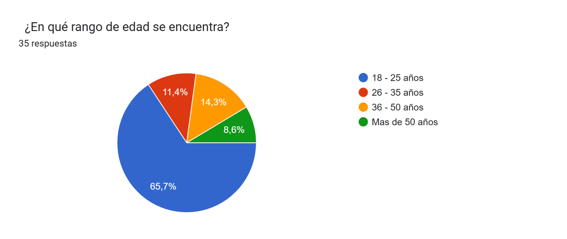
\includegraphics[width=0.8\textwidth]{figuras/pregunta1.png}
	\caption{Distribución por rango de edad de los encuestados.}
	\label{fig:rango_edad}
\end{figure}
Resultados: El 65.7\% de los encuestados tiene entre 18 y 25 años, seguido por el grupo de 36 a 50 años (14.3\%), 26 a 35 años (11.4\%) y mayores de 50 años (8.6\%).

Análisis: La muestra refleja una población predominantemente joven y con alta probabilidad de ser nativa o activa digitalmente. Esto sugiere que la curva de aprendizaje para utilizar la interfaz de usuario en será mínima, favoreciendo una adopción rápida del sistema.
\end{minipage}

\vspace{1cm}


\noindent
\begin{minipage}{\textwidth}
	\textbf{Pregunta.2}
	\begin{figure}[H]
		\centering
		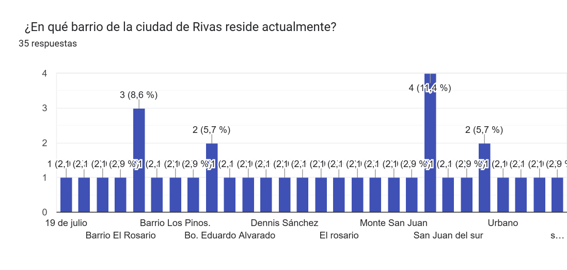
\includegraphics[width=0.8\textwidth]{figuras/pregunta2.png}
		\caption{Distribución de encuestados por barrio de residencia en la ciudad de Rivas.}
		\label{fig:barrio_residencia}
	\end{figure}
	Resultados: Se registró participación de múltiples sectores, destacando barrios como Gaspar García Laviana, San Francisco, Popoyuapa y Eduardo Alvarado, abarcando tanto zonas céntricas como retiradas del municipio.
	
	Análisis: La diversidad de ubicaciones de las cuales se reportarian insidencias confirma la necesidad de estructurar un modelo relacional normalizado (MR-02) que gestione catálogos de departamentos, municipios y sectores, asegurando que las incidencias puedan agruparse y visualizarse correctamente en los mapas de calor para la administración.
\end{minipage}

\vspace{1cm}

\noindent
\begin{minipage}{\textwidth}
	\textbf{Pregunta.3}
	\begin{figure}[H]
		\centering
		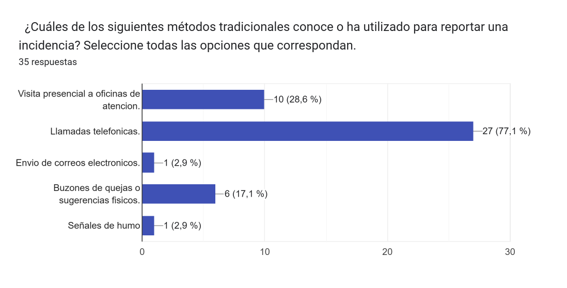
\includegraphics[width=0.8\textwidth]{figuras/pregunta3.png}
		\caption{Métodos tradicionales conocidos o utilizados por la ciudadanía para reportar incidencias.}
		\label{fig:metodos_tradicionales}
	\end{figure}
	Resultados: Las llamadas telefónicas son el medio predominante (presente con el 77\% ). Las visitas presenciales a oficinas de atención ocupan el segundo lugar (presentes en el 28.6\% de las respuestas), mientras que otros metodos tienen menos relevancia.
	
	Análisis: Existe una fuerte dependencia de métodos que requieren atención inmediata de un operador o desplazamiento físico. Esto podria generar cuellos de botella para las entidades, de esa forma un sistema asíncrono y digital que reciba incidencias 24/7 sin saturar mitigaria este problema .
\end{minipage}

\vspace{1cm}

\noindent
\begin{minipage}{\textwidth}
	\textbf{Pregunta.4}
	\begin{figure}[H]
		\centering
		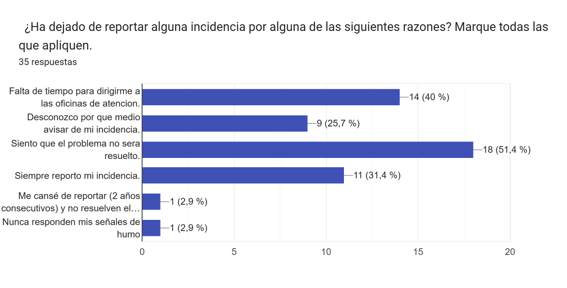
\includegraphics[width=0.8\textwidth]{figuras/pregunta4.png}
		\caption{Principales motivos por los cuales los ciudadanos han desistido de reportar una incidencia.}
		\label{fig:razones_abandono}
	\end{figure}
	Resultados: La percepción de que "el problema no será resuelto" es el factor de desmotivación más fuerte (presente con el 51.4\% de las respuestas totales). La "falta de tiempo para dirigirse a las oficinas" le sigue de cerca (presente en el 40\% de las respuestas).
	
	Análisis: La apatía por falta de resultado es una barrera crítica. La plataforma Comunica eliminará la barrera del tiempo mediante el acceso remoto y mitigará la percepción de inacción al mostrar el avance real de cada caso.
\end{minipage}

\vspace{1cm}

\noindent
\begin{minipage}{\textwidth}
	\textbf{Pregunta.5}
	\begin{figure}[H]
		\centering
		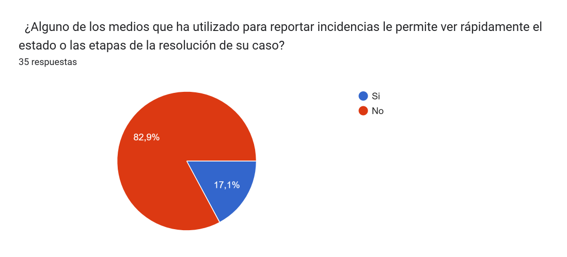
\includegraphics[width=0.8\textwidth]{figuras/pregunta5.png}
		\caption{Visibilidad del estado y etapas de resolución a través de los medios de reporte actuales.}
		\label{fig:visibilidad_estado}
	\end{figure}
	Resultados: El 82.9\% de los encuestados indicó que "No".
	
	Análisis: Queda en evidencia una severa carencia de seguimiento visible en los procesos actuales. Este vacío justifica el desarrollo del módulo de seguimiento (MR-05) para que los usuarios visualicen transiciones de estado estructuradas (Pendiente, En Proceso, Resuelto).
\end{minipage}

\vspace{1cm}

\noindent
\begin{minipage}{\textwidth}
	\textbf{Pregunta.6}
	\begin{figure}[H]
		\centering
		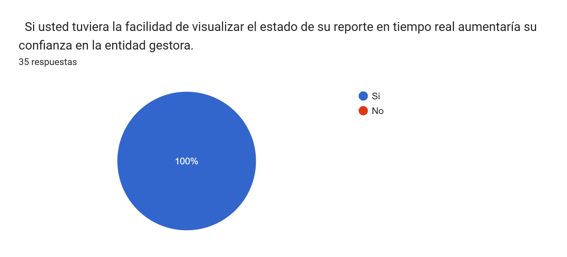
\includegraphics[width=0.8\textwidth]{figuras/pregunta6.png}
		\caption{Impacto de la visualización del estado del reporte en tiempo real sobre la confianza ciudadana.}
		\label{fig:confianza_tiempo_real}
	\end{figure}
	Resultados: El 100\% de los encuestados respondió afirmativamente.
	
	Análisis: Este es el indicador más contundente del estudio. Demuestra que la transparencia digital tiene relación directa con respecto a la confianza ciudadana, validando el impacto social y la  propuesta de un frontend informativo.
\end{minipage}

\vspace{1cm}

\noindent
\begin{minipage}{\textwidth}
	\textbf{Pregunta.7}
	\begin{figure}[H]
		\centering
		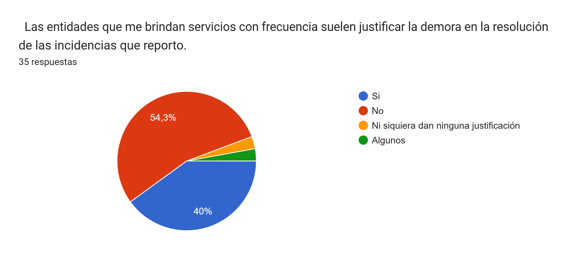
\includegraphics[width=0.8\textwidth]{figuras/pregunta7.png}
		\caption{Frecuencia percibida con la que las entidades justifican las demoras en la resolución de incidencias.}
		\label{fig:justificacion_demoras}
	\end{figure}
	Resultados: El 54.3\% afirma que las entidades no justifican las demoras, frente a un 40\% que indica que sí lo hacen.
	
	Análisis: Existe una deficiencia en la comunicación bidireccional. La falta de justificaciones eleva la percepción de negligencia por parte de las entidades.
\end{minipage}

\vspace{1cm}

\noindent
\begin{minipage}{\textwidth}
	\textbf{Pregunta.8}
	\begin{figure}[H]
		\centering
		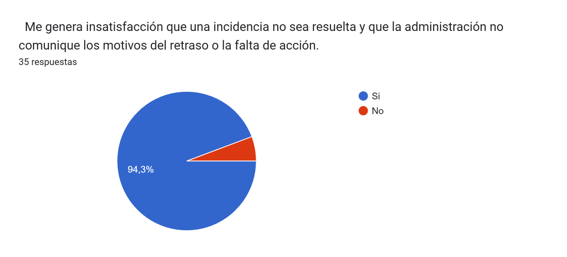
\includegraphics[width=0.8\textwidth]{figuras/pregunta8.png}
		\caption{Nivel de insatisfacción frente a la falta de resolución y ausencia de comunicación institucional.}
		\label{fig:insatisfaccion_retrasos}
	\end{figure}
	Resultados: Al 94.3\% de los usuarios le genera insatisfacción esta falta de comunicación.
	
	Análisis: Se valida la necesidad de que el personal autorizado cuente con herramientas en su panel administrativo para registrar notas de seguimiento y avances (Historia de Usuario HU-15), documentando las razones técnicas de cualquier retraso.
\end{minipage}

\vspace{1cm}

\noindent
\begin{minipage}{\textwidth}
	\textbf{Pregunta.9}
	\begin{figure}[H]
		\centering
		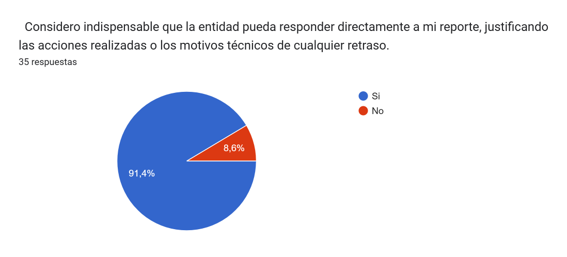
\includegraphics[width=0.8\textwidth]{figuras/pregunta9.png}
		\caption{Importancia ciudadana de recibir respuestas directas y justificaciones técnicas por retrasos.}
		\label{fig:respuesta_directa}
	\end{figure}
	Resultados: El 91.4\% considera esta función como indispensable.
	
	Análisis: Refuerza el punto anterior. El sistema no solo debe ser un buzón digital de entrada, sino un canal de comunicación donde se refleje las actuaciones de la entidad proveedora.
\end{minipage}

\vspace{1cm}

\noindent
\begin{minipage}{\textwidth}
	\textbf{Pregunta.10}
	\begin{figure}[H]
		\centering
		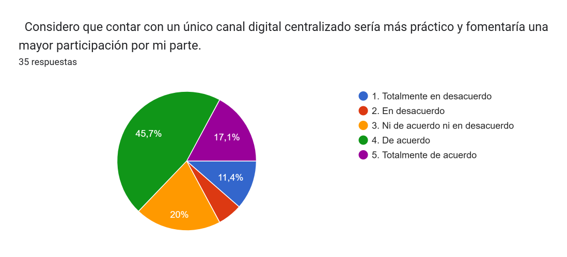
\includegraphics[width=0.8\textwidth]{figuras/pregunta10.png}
		\caption{Percepción ciudadana sobre la practicidad y el fomento de participación de un canal digital centralizado.}
		\label{fig:canal_centralizado}
	\end{figure}
	Resultados: Se mostró una postura favorable del (45.7\% "De acuerdo" y 17.1\% "Totalmente de acuerdo").
	
	Análisis: La unificación de canales dispersos (teléfono, correo, visitas) en una sola plataforma web es percibida como una mejora práctica, lo cual sustenta la viabilidad operativa de centralizar la gestión.
\end{minipage}

\vspace{1cm}

\noindent
\begin{minipage}{\textwidth}
	\textbf{Pregunta.11}
	\begin{figure}[H]
		\centering
		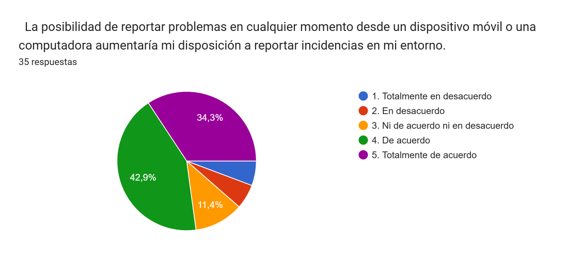
\includegraphics[width=0.8\textwidth]{figuras/pregunta11.png}
		\caption{Aumento en la disposición de participación ciudadana gracias al uso de plataformas en dispositivos móviles y computadoras.}
		\label{fig:disposicion_movil}
	\end{figure}
	Resultados: El 77.2\% respaldó esta afirmación (42.9\% "De acuerdo", 34.3\% "Totalmente de acuerdo").
	
	Análisis: El que la plataforma pueda adaptarse a multiples dispositivos móviles es un factor necesario para la adopción. Esto confirma que el diseño (adaptable a diferentes resoluciones de pantalla en dispositivos móviles y de escritorio).
\end{minipage}

\vspace{1cm}

\noindent
\begin{minipage}{\textwidth}
	\textbf{Pregunta.12}
	\begin{figure}[H]
		\centering
		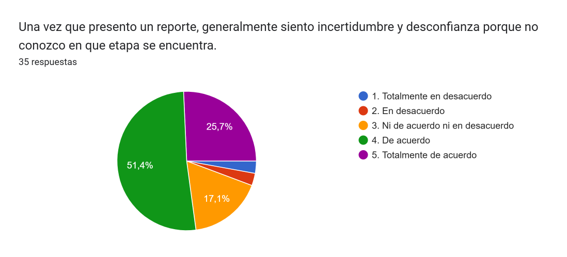
\includegraphics[width=0.8\textwidth]{figuras/pregunta12.png}
		\caption{Nivel de incertidumbre y desconfianza generada por el desconocimiento de las etapas del reporte.}
		\label{fig:incertidumbre_estado}
	\end{figure}
	Resultados: El 77.1\% de la muestra experimenta incertidumbre post-reporte (51.4\% "De acuerdo", 25.7\% "Totalmente de acuerdo").
	
	Análisis: Este sentimiento es el producto directo de usar canales que carecen de seguimiento. El historial interactivo de Comunica resolverá directamente esta necesidad.
\end{minipage}

\vspace{1cm}

\noindent
\begin{minipage}{\textwidth}
	\textbf{Pregunta.13}
	\begin{figure}[H]
		\centering
		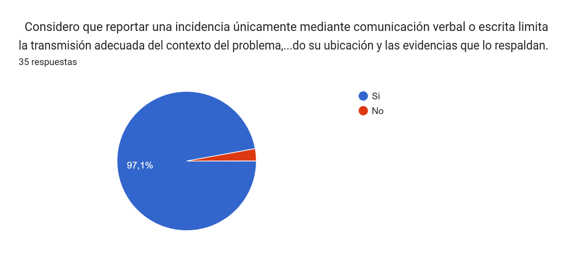
\includegraphics[width=0.8\textwidth]{figuras/pregunta13.png}
		\caption{Percepción ciudadana respecto a las limitaciones descriptivas y de contexto en la comunicación verbal o escrita.}
		\label{fig:limitacion_contexto}
	\end{figure}
	Resultados: Un abrumador 97.1\% indicó que "Sí".
	
	Análisis: Justificación para el meta-requisito MR-03. La integración de captura con respecto a coordenadas exactas y la gestión de evidencias visuales que son necesidades técnicas  para superar las limitaciones del modelo tradicional.
\end{minipage}

\vspace{1cm}

\noindent
\begin{minipage}{\textwidth}
	\textbf{Pregunta.14}
	\begin{figure}[H]
		\centering
		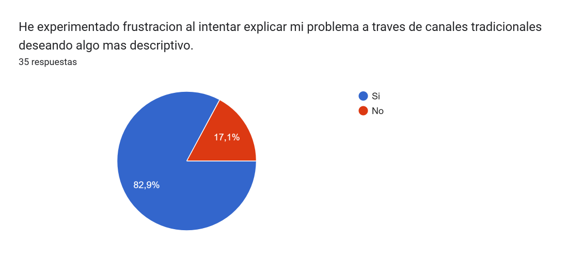
\includegraphics[width=0.8\textwidth]{figuras/pregunta14.png}
		\caption{Nivel de frustración experimentado al utilizar canales tradicionales carentes de soporte visual y descriptivo.}
		\label{fig:frustracion_tradicional}
	\end{figure}
	Resultados: El 82.9\% ha sentido esta frustración.
	
	Análisis: Relacionado directamente con la pregunta anterior, demuestra que las descripciones textuales o telefónicas son insuficientes para reportes de infraestructura, requiriendo el apoyo de otras funcionalidades.
\end{minipage}

\vspace{1cm}

\noindent
\begin{minipage}{\textwidth}
	\textbf{Pregunta.15}
	\begin{figure}[H]
		\centering
		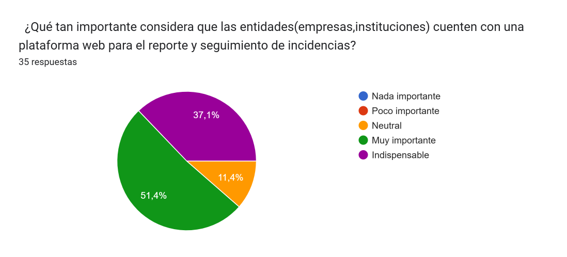
\includegraphics[width=0.8\textwidth]{figuras/pregunta15.png}
		\caption{Nivel de importancia general atribuido a la implementación de una plataforma web para la gestión de incidencias.}
		\label{fig:importancia_plataforma}
	\end{figure}
   Resultados: El 88.5\% lo califica como altamente relevante (51.4\% "Muy importante", 37.1\% "Indispensable"). El 11.4\% restante se mantuvo neutral. \
   Análisis: Representa la validación final del proyecto. Existe un consenso ciudadano sobre la urgencia y el valor de modernizar la atención de servicios mediante soluciones informáticas estructuradas, respaldando la ejecución completa del desarrollo.
\end{minipage}
\vspace{1cm}

Los resultados obtenidos a través de este instrumento aplicado para la recolección de datos primarios evidencian de manera contundente las deficiencias comunicativas y operativas de los métodos tradicionales de atención en el municipio de Rivas. La dependencia de canales que carecen de trazabilidad genera un ciclo de incertidumbre, frustración y desconfianza ciudadana. Frente a esta problemática, la encuesta demuestra una aceptación y disposición casi unánime hacia la adopción de un canal digital centralizado. La exigencia ciudadana por contar con seguimiento en tiempo real, georreferenciación exacta, soporte de evidencia multimedia y retroalimentación con la entidad, no solo reafirma las problemáticas planteadas en la fase diagnóstica, sino que justifica empíricamente los meta-requisitos técnicos y funcionales definidos para Comunica. De este modo, se consolida la viabilidad operativa y el impacto social del proyecto, sentando las bases definitivas para la etapa de diseño y desarrollo de la plataforma.

\textbf{4.\hypertarget{subsec:requerimentos}{OE1} Identificación de requerimientos}

A partir del análisis documental y de campo, se definieron siete requerimientos (\textbf{MR-01} al \textbf{MR-07}) que delimitan el alcance funcional y técnico de la plataforma «Comunica». En conjunto, estos requerimientos cubren cuatro dimensiones esenciales del sistema:

\begin{itemize}
	\item \textbf{Seguridad y control de acceso (MR-01):} Garantiza la autenticación de usuarios y la diferenciación de permisos según su rol operativo (ciudadanía, personal institucional y administradores).
	\item \textbf{Captura y organización territorial (MR-02 y MR-03):} Estructura la división geográfica administrativa para ubicar cada reporte y provee un mecanismo interactivo con geolocalización y evidencia multimedia.
	\item \textbf{Enrutamiento y seguimiento operativo (MR-04 y MR-05):} Automatiza la clasificación por tipología hacia la entidad competente y asegura la trazabilidad completa durante todo el ciclo de vida de la incidencia.
	\item \textbf{Analítica y calidad del sistema (MR-06 y MR-07):} Consolida indicadores de desempeño en paneles visuales, respaldados por una arquitectura que garantiza integridad transaccional, seguridad y alto rendimiento.
\end{itemize}
 Para una vista especifica de los requerimentos del proyecto revise los Metarequisitos plasmados en la \textbf{\hyperlink{subsec:matriz}{Matriz de Trazabilidad}} 
 
 \textbf{5.\hypertarget{subsec:backlog}{OE1} \hyperlink{subsec:backlog1}{Cómo resultado del plan de historias usuarios se concreto el Backlog, este se encuentra en la página 60, toque para visualizar}}
 
 \textbf{Resultados del objetivo 2}

 \textbf{1.\hypertarget{subsec:arquitecturaSoftware}{OE2.Arquitectura de software}} \textbf{\hyperlink{subsec:viabiTec}{El resultado de esta acción, se consolida en la definición y justificación teórica de la arquitectura del software, documentada a detalle en el apartado de Viabilidad Técnica.}} Este resultado establece una separación clara de responsabilidades bajo un modelo cliente-servidor, designando a Angular para la interfaz interactiva de usuario (frontend), a AdonisJS para la API REST y la lógica de negocio, y a PostgreSQL para la persistencia de datos. Además, define los lineamientos para la autenticación, el control de acceso basado en roles (RBAC) y la distribución de la infraestructura apoyada en servicios en la nube como Render, Netlify y Cloudinary. Con esta fundamentación, el equipo de desarrollo cuenta con los requerimientos técnicos y las responsabilidades operativas de cada componente completamente delimitados, asegurando la base estructural necesaria para guiar la etapa de construcción del sistema.
 
  \vspace{1cm}
 
 \noindent
 \begin{minipage}{\textwidth}
 \textbf{2.OE2 \hypertarget{subsec:modeloBaseDatos}{Modelo de base de datos}} 
 , En esta sección se define la estructura lógica y física de la base de datos relacional del sistema Comunica, implementada en PostgreSQL.se muestra la organización de las tablas principales como usuarios, incidencias, categorías, ubicaciones con el resultado de Modelo de
 datos preparado para respaldar el registro y seguimiento de las incidencias:
 
 	  \begin{figure}[H]
 		\centering
 		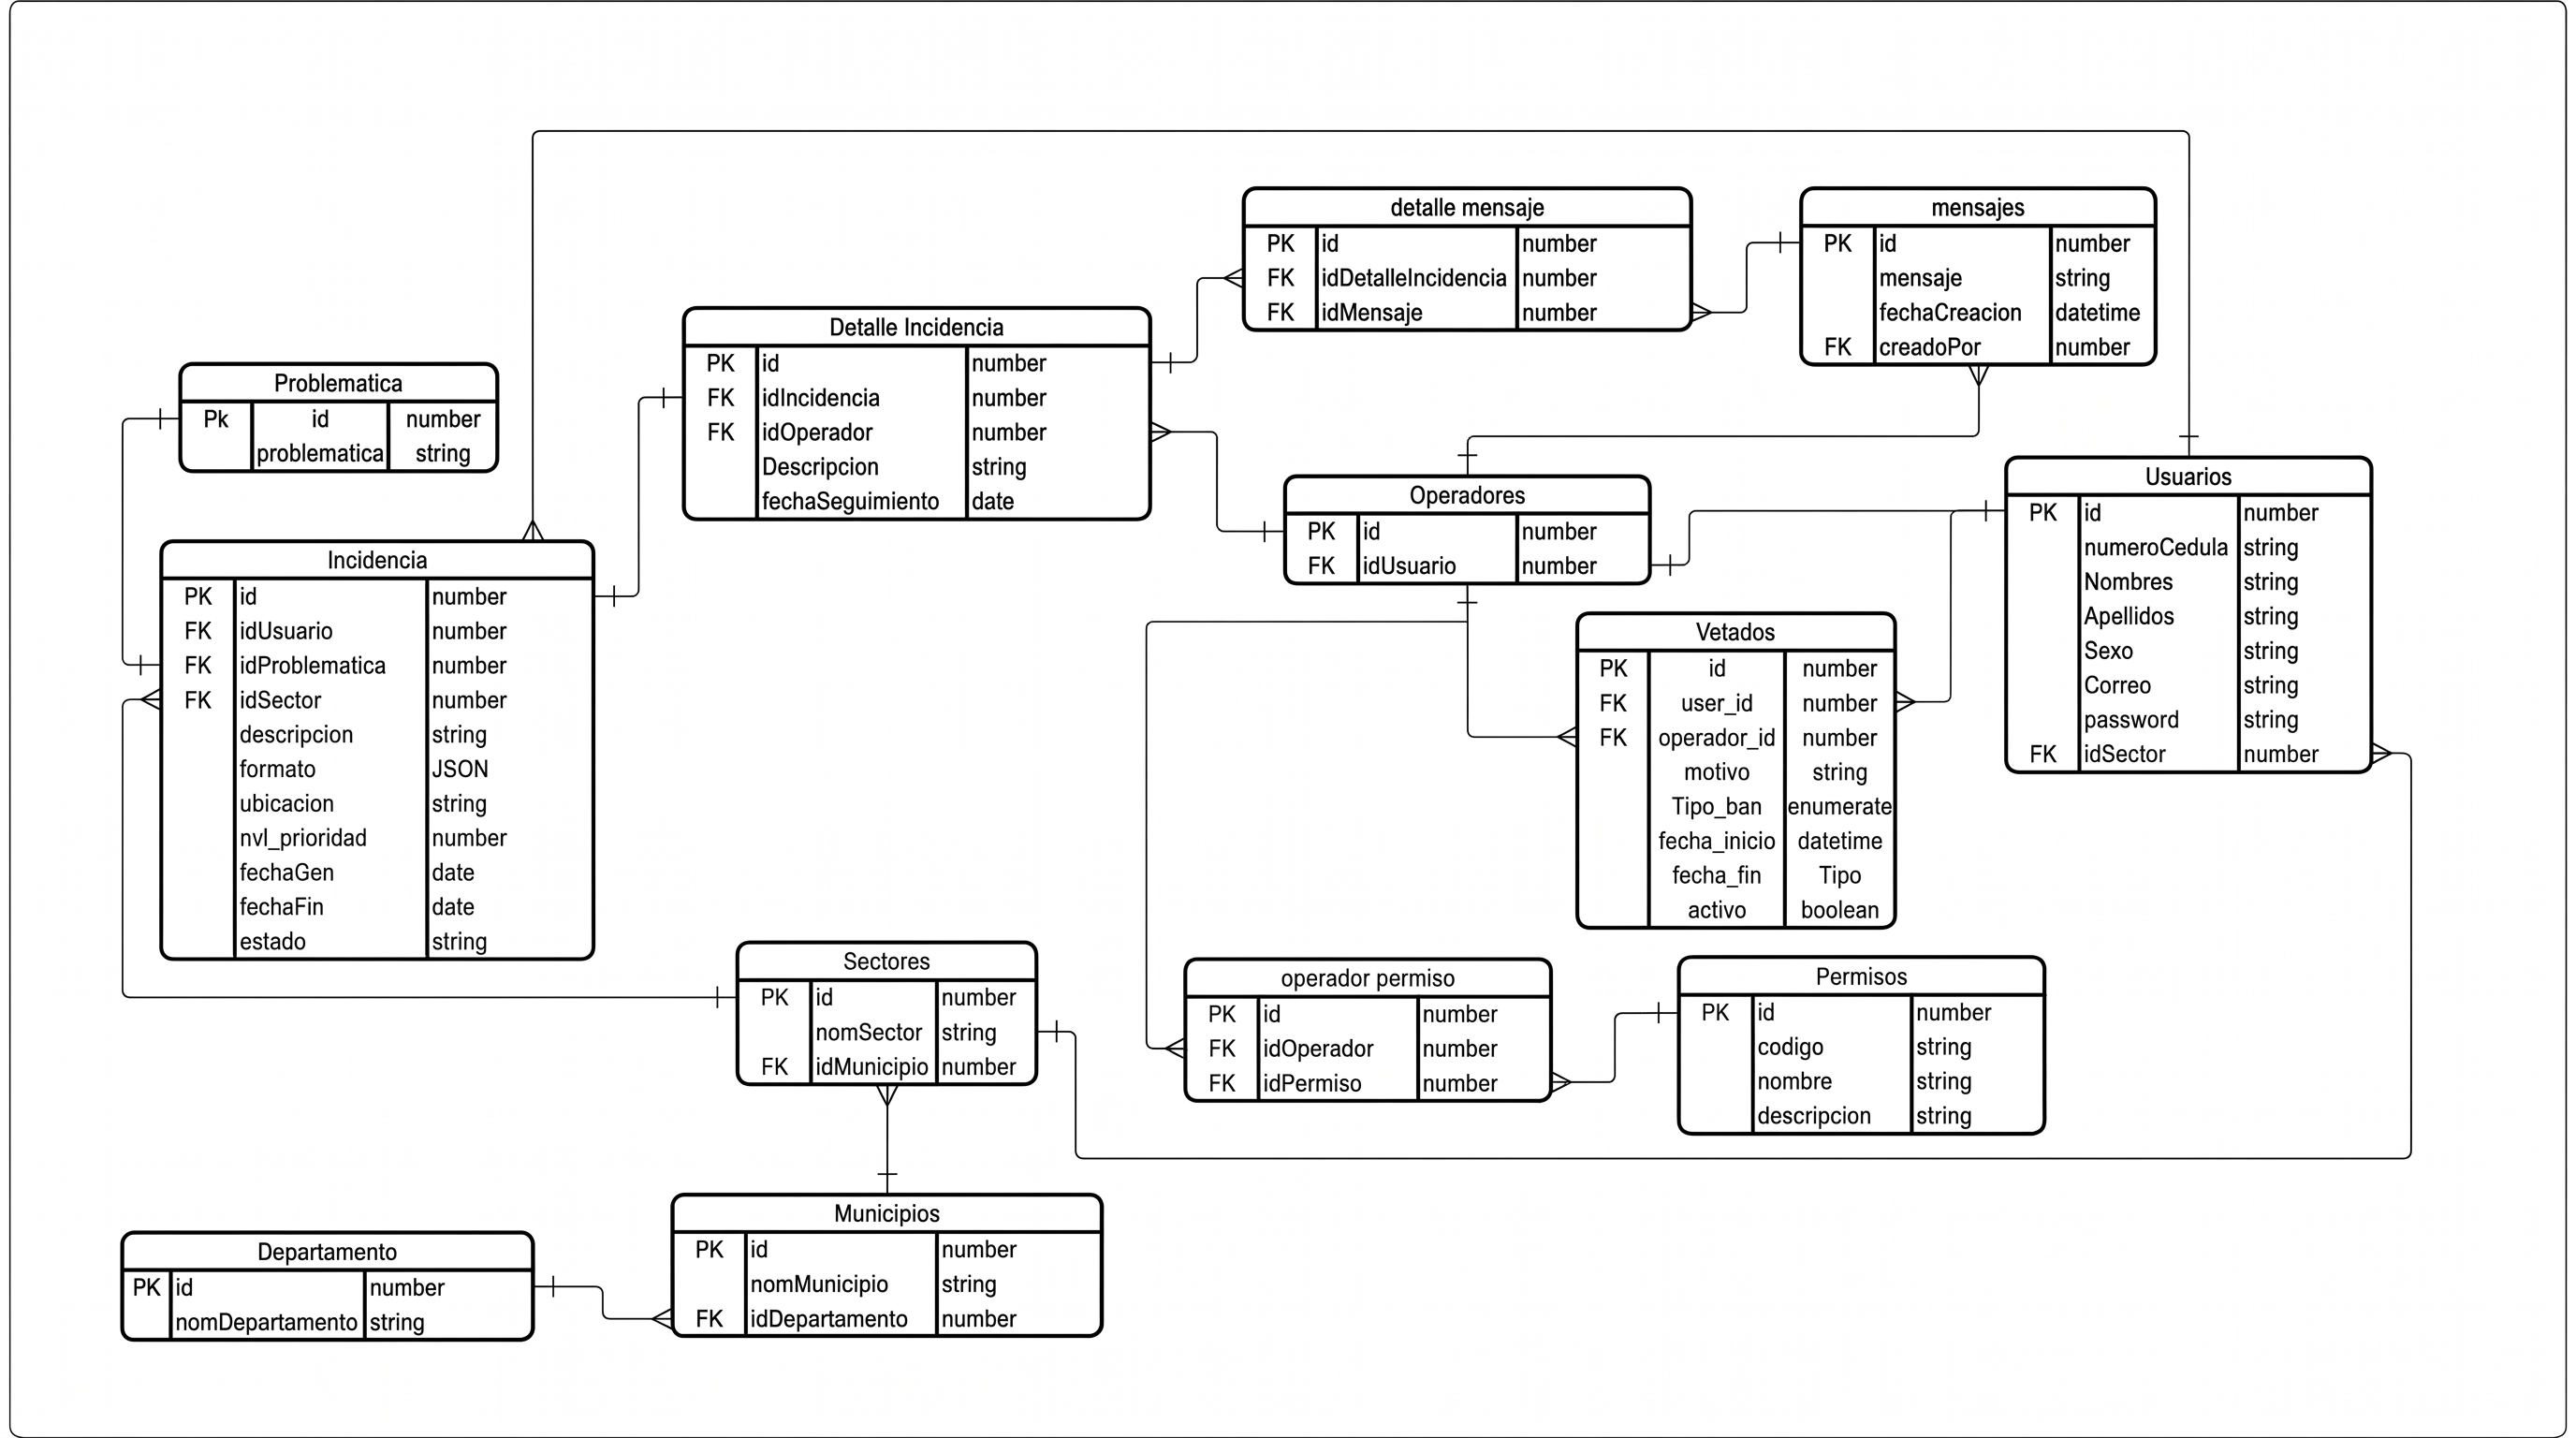
\includegraphics[width=0.8\textwidth]{figuras/diagramaEntidadR.jpg}
 		
 		\caption{Diagrama entidad relación.}
 		\label{fig:Entidad relacion}
 		\end{figure}
 		El Diagrama Entidad-Relación estructura la base de datos de la plataforma Comunica en trece tablas distribuidas en cuatro bloques funcionales que garantizan la integridad referencial del sistema. La organización geográfica se establece de forma jerárquica mediante las entidades Departamento, Municipios y Sectores, mientras que la gestión de cuentas, los privilegios operativos basados en roles y las sanciones por uso indebido se controlan a través de las tablas Usuarios, Operadores, Permisos, operador permiso y Vetados. Por su parte, el ciclo de vida de los reportes se concentra en la entidad Incidencia —la cual almacena la descripción, ubicación, nivel de prioridad, estado y metadatos en formato JSON clasificados según su Problematica—, vinculándose con Detalle Incidencia, detalle mensaje y mensajes para conservar el historial cronológico de seguimiento y las respuestas institucionales dirigidas al ciudadano.
 \end{minipage}
 \vspace{1cm}
 
 
 \textbf{3.OE3 \hypertarget{subsec:disenoInterfaces}{Diseño de interfaces UI/UX}}
 
 En esta sección se definen los prototipos de interfaz, los flujos de navegación y la revisión de usabilidad de la plataforma Comunica, diferenciados según el rol operativo del usuario. El diseño contempla vistas web responsivas para el registro de incidencias por parte del usuario con selección geográfica mediante un mapa interactivo junto con la carga de evidencia fotográfica, un módulo para la consulta del historial y estados de seguimiento, y un panel administrativo para el monitoreo de indicadores y distribución espacial de los reportes en el municipio de Rivas.
 
 \vspace{0.3cm}
 \noindent\textbf{1. Prototipos de interfaz del sistema}
 \vspace{0.2cm}
 

 	\textbf{Interfaz 1. Formulario de Registro de Incidencia}
 	\begin{figure}[H]
 		\centering
 		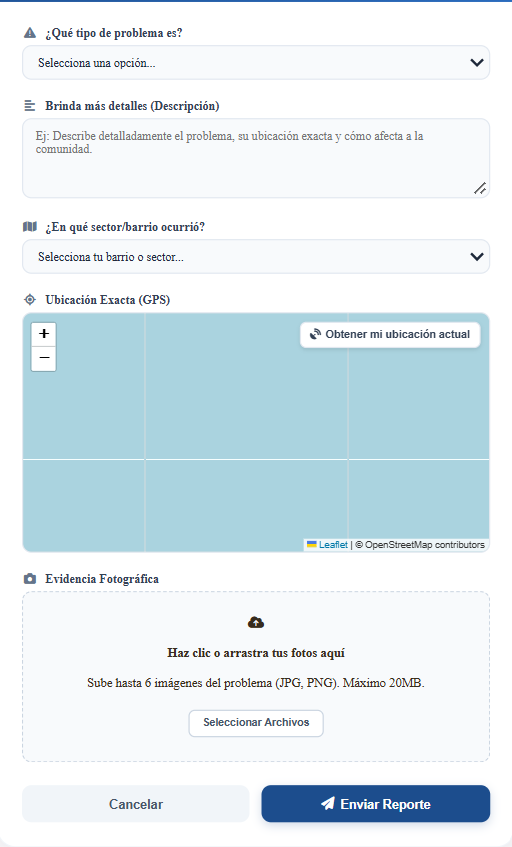
\includegraphics[width=0.55\textwidth]{figuras/reporte.png}
 		\caption{Formulario interactivo para el registro de incidencias con geolocalización GPS y carga de evidencia multimedia.}
 		\label{fig:interfaz_reporte}
 	\end{figure}
 	Descripción: Vista orientada al usuario que estructura la captura del reporte en cinco bloques secuenciales: selección del catálogo de problemáticas, descripción detallada del suceso, asignación del barrio o sector correspondiente, selección de coordenadas exactas mediante un visor cartográfico (con botón de captura automática de ubicación GPS) y un contenedor para adjuntar hasta 6 imágenes de evidencia (formatos JPG o PNG, máximo 20 MB).
 	
 	Análisis: Cumple con el requerimiento de recolección estructurada y georreferenciada del objetivo OE2, reduciendo la ambigüedad en la ubicación de los daños reportados por la comunidad.
 
 
 \vspace{0.5cm}
 
 \begin{minipage}{\textwidth}
 	\textbf{Interfaz 2. Historial de Reportes y Consulta de Estados}
 	\begin{figure}[H]
 		\centering
 		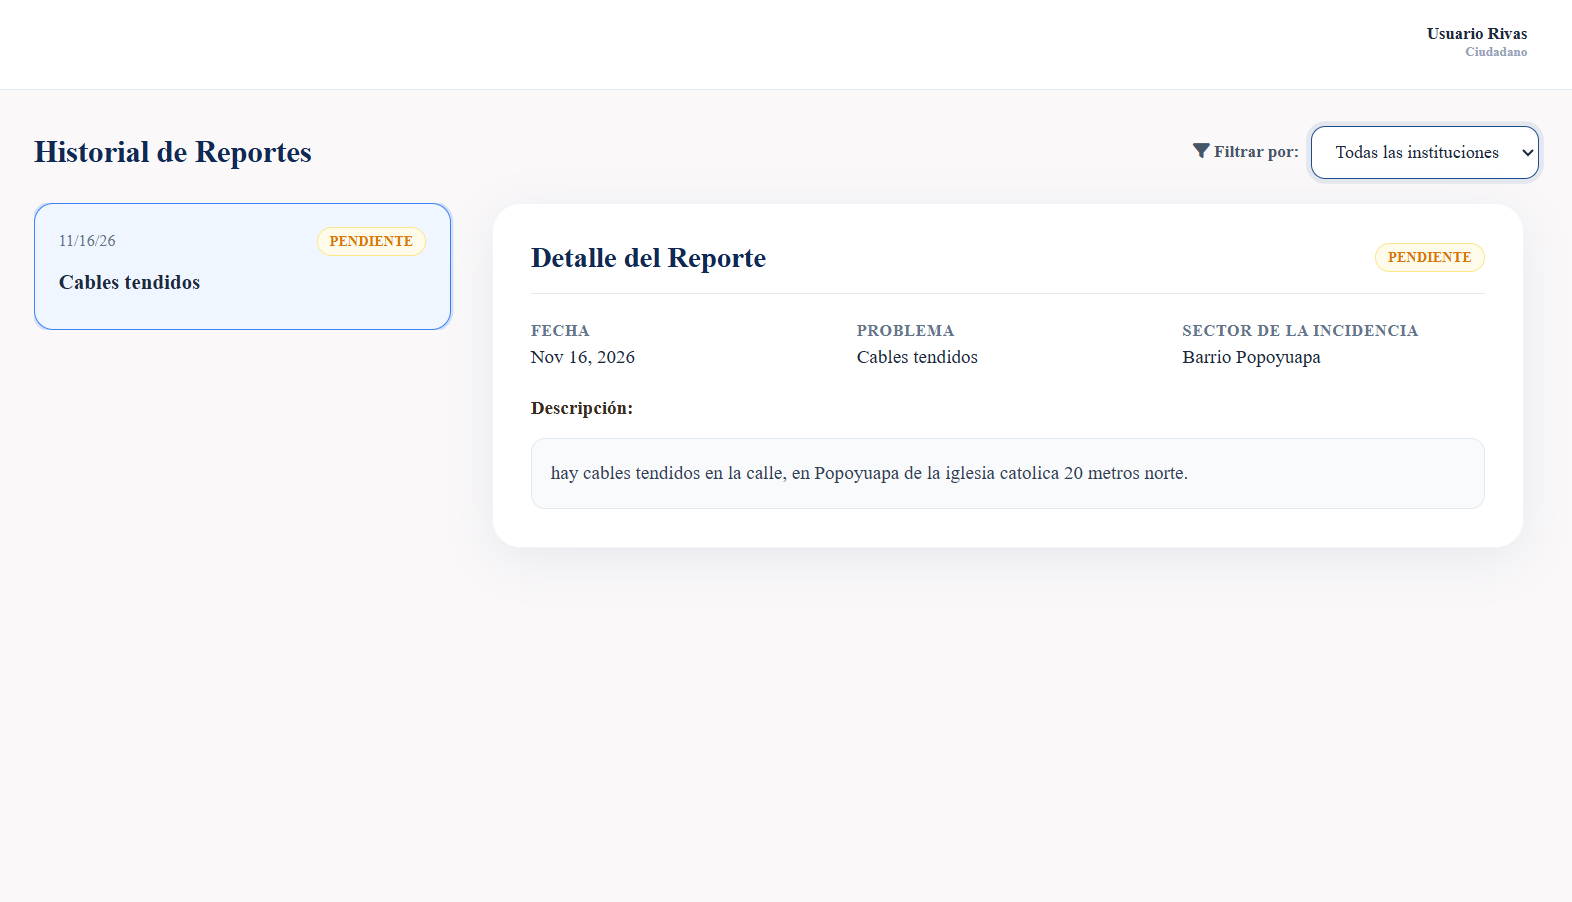
\includegraphics[width=0.8\textwidth]{figuras/historialUser.png}
 		\caption{Vista de historial de reportes enviados y panel de consulta detallada de estado.}
 		\label{fig:interfaz_historial}
 	\end{figure}
 	Descripción: Interfaz de seguimiento para el rol usuario que emplea un diseño de vista dividida. En el panel izquierdo se listan cronológicamente las incidencias registradas con su etiqueta de estado actual (Pendiente, En Proceso, Resuelto), mientras que en la parte derecha se despliega el detalle completo del caso seleccionado (fecha, tipo de problema, sector como el Barrio Popoyuapa y descripción), incorporando además un selector superior para filtrar reportes.
 	
 	Análisis: Garantiza la trazabilidad y transparencia hacia el usuario, permitiéndole verificar en tiempo real el progreso de atención de sus solicitudes sin necesidad de acudir presencialmente a la municipalidad o realizar llamadas.
 \end{minipage}
 
 \vspace{0.5cm}
 
 \begin{minipage}{\textwidth}
 	\textbf{Interfaz 3. Panel de Control Administrativo de la entidad}
 	\begin{figure}[H]
 		\centering
 		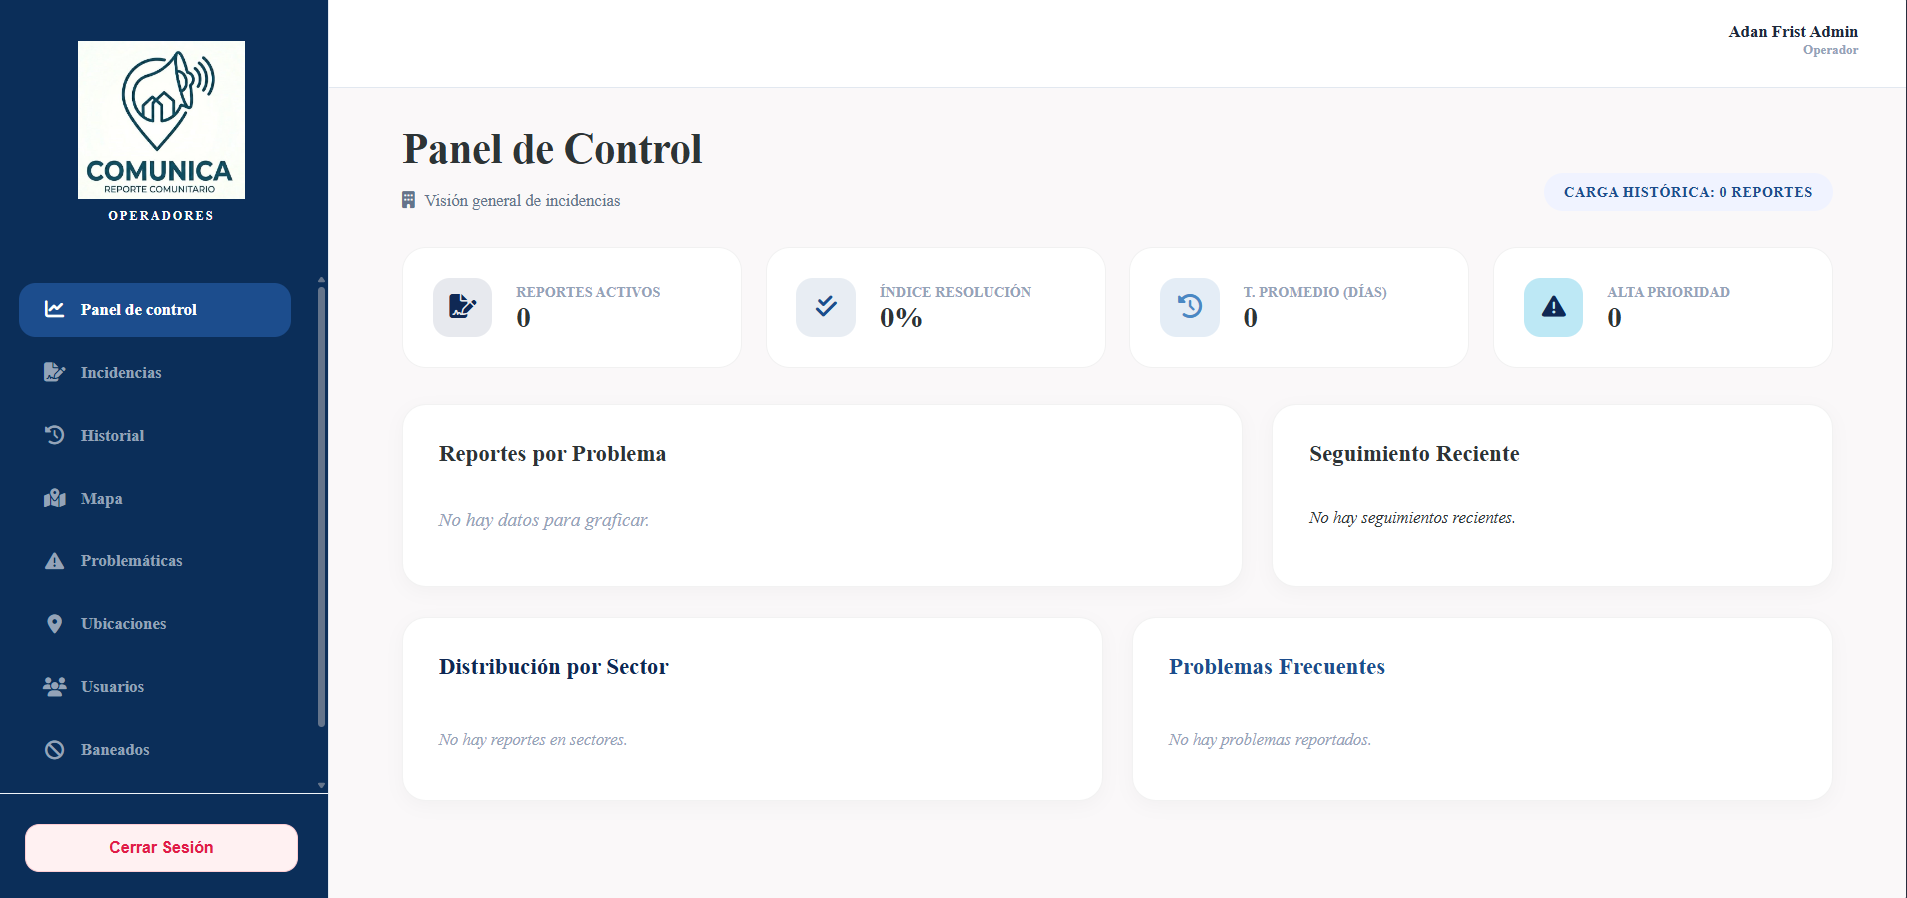
\includegraphics[width=0.8\textwidth]{figuras/panelAdministrativo.png}
 		\caption{Panel administrativo con indicadores clave de rendimiento y distribución analítica de incidencias.}
 		\label{fig:interfaz_panel_admin}
 	\end{figure}
 	Descripción: Entorno principal de trabajo para el rol de Operador y Administrador. Incorpora una barra lateral de navegación hacia los módulos del sistema (\textit{Panel de control, Incidencias, Historial, Mapa, Problemáticas, Ubicaciones, Usuarios y Baneados}) y un área central con cuatro tarjetas de métricas importantes (reportes activos, índice de resolución porcentual, tiempo promedio en días e incidencias de alta prioridad), complementadas por paneles analíticos para graficar reportes por problema, seguimiento reciente, distribución por sector y problemas frecuentes.
 	
 	Análisis: Centraliza la supervisión operativa, facilitando la toma de decisiones basada en datos sobre las zonas y tipologías de fallo con mayor demanda de atención.
 \end{minipage}
 
 \vspace{0.5cm}
 
 \begin{minipage}{\textwidth}
 	\textbf{Interfaz 4. Mapa General de Reportes para Operadores}
 	\begin{figure}[H]
 		\centering
 		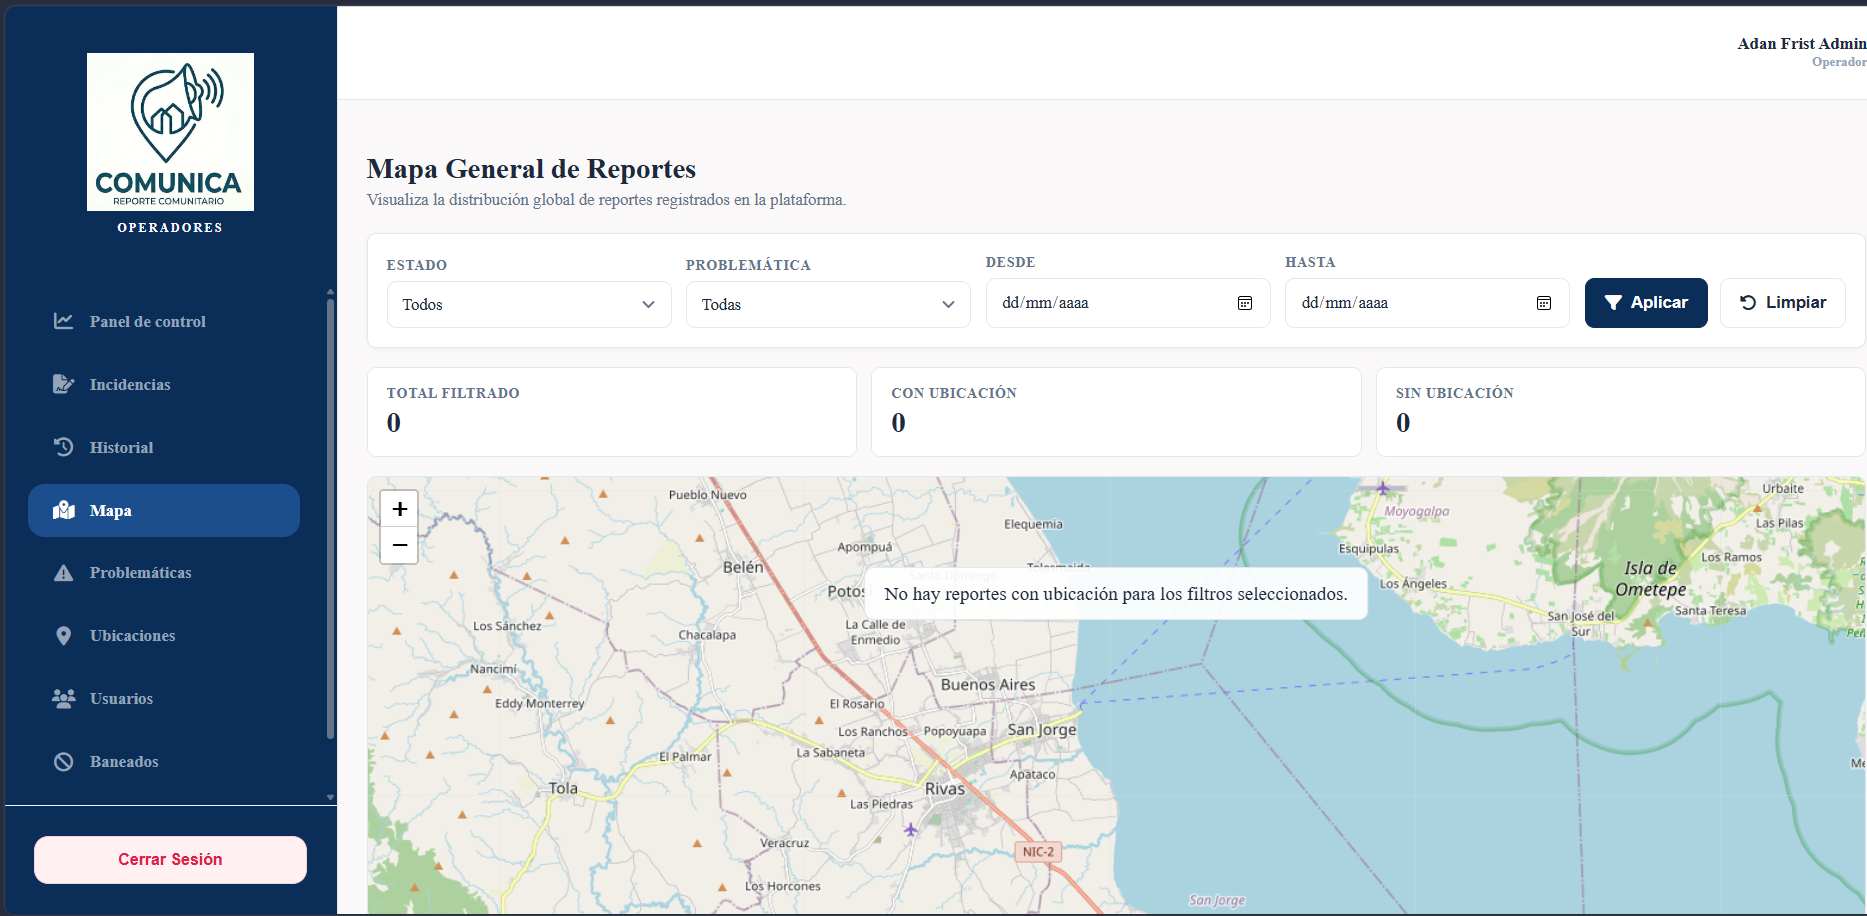
\includegraphics[width=0.8\textwidth]{figuras/mapaInteractivo.png}
 		\caption{Visor cartográfico general con filtros multicriterio para el monitoreo espacial de incidencias en Rivas.}
 		\label{fig:interfaz_mapa_general}
 	\end{figure}
 	Descripción: Herramienta de visualización geoespacial para operadores que proyecta la distribución global de incidencias sobre el mapa del municipio de Rivas. Dispone de una barra de filtrado avanzado por estado, categoría de problemática y rango de fechas (desde/hasta), junto con tres contadores dinámicos (\textit{Total filtrado, Con ubicación y Sin ubicación}) que actualizan en tiempo real los marcadores desplegados en el mapa cartográfico.
 	
 	Análisis: Permite identificar visualmente focos críticos de incidencias por barrio o sector, optimizando la planificación territorial de las cuadrillas de respuesta de la entidad.
 \end{minipage}
 
 \vspace{0.5cm}
 \noindent\textbf{2. Flujos de navegación del sistema}
 \vspace{0.2cm}
 
 La arquitectura de navegación se divide en dos flujos operativos:
 \begin{itemize}
 	\item \textbf{Flujo de navegación del Ciudadano:} Inicia en la vista de autenticación o registro de cuenta $\rightarrow$ accede al panel principal ciudadano $\rightarrow$ selecciona \textit{Crear Reporte} (completando categoría, sector, punto GPS en el mapa interactivo y fotografías) $\rightarrow$ envía el formulario $\rightarrow$ es redirigido a la vista \textit{Historial de Reportes}, donde puede consultar el estado y las notas de seguimiento de cada caso.
 	\item \textbf{Flujo de navegación del Operador / Administrador:} Inicia en la pantalla de autenticación $\rightarrow$ ingresa al \textit{Panel de Control} (visualización de métricas generales) $\rightarrow$ navega mediante el menú lateral hacia \textit{Incidencias} \textit{Mapa} (filtrado geoespacial de reportes), \textit{Problemáticas y Ubicaciones} (gestión de catálogos) o \textit{Usuarios y Baneados} (administración de permisos y aplicación de sanciones por uso indebido).
 \end{itemize}
 
 \vspace{0.3cm}
 \noindent\textbf{3. Revisión de criterios de usabilidad (UI/UX)}
 \vspace{0.2cm}
 
 El diseño de las interfaces fue validado bajo principios de usabilidad y diseño centrado en el usuario para asegurar su adopción técnica y comunitaria:
 
 \begin{itemize}
 	\item \textbf{Claridad visual y jerarquía tipográfica:} Uso de una paleta cromática de alto contraste (azul marino oscuro en navegación lateral sobre lienzos blancos y grises claros) que facilita la lectura de formularios y métricas.
 	\item \textbf{Retroalimentación visual de estados:} Implementación de etiquetas semánticas codificadas por color (como el indicador amarillo para el estado \textit{PENDIENTE}) y contadores numéricos claros que informan de inmediato la situación de cada reporte.
 	\item \textbf{Prevención de errores y asistencia al usuario:} Inclusión de textos de ayuda contextuales (\textit{placeholders}), selectores desplegables vinculados a los catálogos de informacion, límites explícitos de carga multimedia (máximo 6 archivos y 20 MB) y geolocalización asistida por un solo clic.
 	\item \textbf{Diseño responsivo y adaptabilidad:} Estructura modular basada en tarjetas y contenedores flexibles que se ajustan tanto a pantallas móviles para el reporte ciudadano en campo como a monitores de escritorio para la gestión administrativa.
 \end{itemize}

 
 \hypertarget{subsec:modeladoFlujo}{Modelado del flujo de incidencias}
 
}
% Capítulo 5: Conclusiones
% Propósito: Sintetizar las conclusiones obtenidas en función de los objetivos alcanzados y plantear recomendaciones o trabajos futuros.
\section{Recomendaciones}

A partir del desarrollo de la presente investigación, se establecen recomendaciones orientadas al fortalecimiento de la plataforma web Comunica y al desarrollo de futuras investigaciones relacionadas con la gestión digital de incidencias y la optimización de los procesos de atención al usuario.

Se recomienda realizar un estudio de mercado dirigido entidades que ofertan servicios del municipio de Rivas, con el propósito de identificar entidades interesadas en adoptar Comunica. Este estudio permitirá conocer sus necesidades, evaluar la aceptación de la plataforma y determinar la viabilidad de su comercialización, considerando el precio propuesto y las condiciones de adquisición.

Se recomienda fortalecer las evaluaciones de usabilidad y accesibilidad mediante la participación de usuarios con diferentes niveles de conocimientos tecnológicos. Esto permitirá identificar dificultades de navegación, comprensión y utilización de las funcionalidades, contribuyendo a que Comunica ofrezca una experiencia de uso más intuitiva y accesible.

Asimismo, se recomienda realizar pruebas de rendimiento, seguridad y escalabilidad que permitan evaluar el comportamiento de la plataforma ante diferentes cargas de trabajo. Estas evaluaciones contribuirán a identificar posibles limitaciones técnicas y establecer las mejoras necesarias para garantizar la estabilidad, protección de la información y capacidad de crecimiento del sistema.

Para futuras investigaciones relacionadas con el desarrollo de plataformas de gestión de incidencias, se recomienda incorporar las buenas prácticas de ITIL 4, particularmente en los procesos de registro, clasificación, priorización, asignación, seguimiento y cierre de reportes. Su aplicación permitirá orientar la gestión de incidencias mediante procedimientos estructurados y criterios de evaluación que favorezcan la calidad y mejora continua del servicio.

Se recomienda que futuras investigaciones contemplen la evaluación del impacto operativo de las soluciones tecnológicas desarrolladas, mediante indicadores como los tiempos de respuesta, la cantidad de incidencias atendidas y la satisfacción de los usuarios. Esto permitirá obtener evidencia sobre la efectividad de estas herramientas y su contribución a la optimización de los procesos de atención.

De igual manera, se sugiere que otros investigadores adopten metodologías estructuradas como Design Science Research Methodology (DSRM), complementadas con marcos de desarrollo ágil como Scrum y prácticas de Extreme Programming (XP). Su aplicación permitirá mantener una relación coherente entre la identificación del problema, el diseño de la solución, su desarrollo y la evaluación de los resultados obtenidos.

Finalmente, se recomienda promover investigaciones relacionadas con la digitalización de los procesos de atención al usuario en instituciones públicas y empresas privadas de Nicaragua, considerando sus condiciones tecnológicas, organizacionales y sociales. Estos trabajos contribuirán a ampliar los antecedentes nacionales y generar conocimientos que puedan servir como referencia para el desarrollo de nuevas soluciones tecnológicas.
\newpage
\section{Concluciones}

La presente investigación permitió establecer las bases metodológicas, funcionales y tecnológicas para el desarrollo de la plataforma web Comunica, orientada a mejorar los procesos de registro, clasificación y seguimiento de incidencias. A través de la revisión bibliográfica y el estudio de mapeo sistemático, se identificaron soluciones tecnológicas existentes y sus principales aportes, lo que facilitó la definición de las funcionalidades necesarias para atender la problemática planteada.

En relación con el primer objetivo específico, se avanzó en el análisis y definición de los requerimientos funcionales y no funcionales mediante la revisión de investigaciones relacionadas con la gestión digital de incidencias y la identificación de las necesidades asociadas a los mecanismos tradicionales de atención. Este proceso permitió establecer los requisitos de autenticación, registro de reportes, geolocalización, clasificación, seguimiento y administración, así como elaborar un instrumento de recolección de datos para complementar el análisis de las necesidades de los usuarios.

Respecto al segundo objetivo específico, se definió una propuesta de arquitectura tecnológica basada en Angular, AdonisJS y PostgreSQL, junto con el diseño de los componentes necesarios para almacenar y gestionar la información de los reportes. Asimismo, se establecieron los elementos funcionales de las interfaces de usuario, considerando el registro de incidencias con evidencias fotográficas, ubicación geográfica y consulta de estados, proporcionando una estructura para la construcción e integración de la plataforma.

En cuanto al tercer objetivo específico, se estructuró el desarrollo de los módulos funcionales de Comunica mediante historias de usuario, matrices de trazabilidad y actividades organizadas en sprints. Esta planificación permitió relacionar los requerimientos establecidos con los componentes de registro, clasificación, seguimiento y administración de incidencias, incluyendo un panel de indicadores y visualizaciones geográficas. De esta manera, se definieron los criterios funcionales y técnicos que orientan la construcción y evaluación de la solución.

Finalmente, en relación con el objetivo general, la investigación permitió fundamentar y organizar el desarrollo de una plataforma web destinada a centralizar la recepción y gestión de incidencias en un entorno digital. La integración propuesta de mecanismos de registro, seguimiento y análisis de información constituye una base para mejorar la comunicación entre los usuarios y las entidades responsables. No obstante, la comprobación de su contribución efectiva a la optimización de los procesos de atención requiere completar las pruebas funcionales y realizar evaluaciones en condiciones reales de uso.

% ==========================================
% Referencias Bibliográficas
% ==========================================
\printbibliography[heading=bibintoc, title={Referencias}, label={subsec:referencias}]


\end{document}
